\documentclass [xcolor=table] {beamer}

    \usepackage [utf8,francais,multichap] {courspda}

    \hypersetup
    {
	pdfauthor={Pierre David},
        pdfsubject={Systèmes d'exploitation},
	pdftitle={Systèmes d'exploitation},
	pdfkeywords={Systèmes d'exploitation, POSIX, fichiers, répertoires, processus, temps, signaux, tubes}
    }

    \author {Pierre David \texorpdfstring {\\} {} \texttt {pda@unistra.fr}}
\institute {Université de Strasbourg -- Licence d'informatique}
\date {2017 -- 2018}

    \title {Systèmes d'exploitation}

\begin {document}

%%%%%%%%%%%%%%%%%%%%%%%%%%%%%%%%%%%%%%%%%%%%%%%%%%%%%%%%%%%%%%%%%%%%%%%%%%%%%%
% PLAN
%%%%%%%%%%%%%%%%%%%%%%%%%%%%%%%%%%%%%%%%%%%%%%%%%%%%%%%%%%%%%%%%%%%%%%%%%%%%%%

\begin {frame} {Licence d'utilisation}

    \fB

    \copyright Pierre David

    \vspace* {3mm}

    Disponible sur \url {http://github.com/pdav/ens}

    \vspace* {3mm}

    Ces transparents de cours sont placés sous licence « Creative
    Commons Attribution -- Pas d’Utilisation Commerciale 4.0
    International »

    \vspace* {3mm}

    Pour accéder à une copie de cette licence,
    merci de vous rendre à l'adresse
    \url {http://creativecommons.org/licenses/by-nc/4.0/}

    \vspace* {3mm}

    
\includegraphics [scale=.7] {by-nc}
\end {frame}


\def\inc{inc1-intro}

\titreA {Introduction}

%%%%%%%%%%%%%%%%%%%%%%%%%%%%%%%%%%%%%%%%%%%%%%%%%%%%%%%%%%%%%%%%%%%%%%%%%%%%%%
% Organisation de l'UE
%%%%%%%%%%%%%%%%%%%%%%%%%%%%%%%%%%%%%%%%%%%%%%%%%%%%%%%%%%%%%%%%%%%%%%%%%%%%%%

\titreB {Organisation de l'UE}

\begin {frame} {Organisation de l'UE}
    Cours structuré en deux grandes parties~:

    \begin {itemize}
	\item comment s'utilise un système d'exploitation ?

	    \begin {itemize}
		\item utilisation des primitives systèmes avec le
		    langage C
		    \\
		    \implique bon niveau en C

		\item primitives POSIX
		    \\
		    \implique norme internationale

		\item idée : comprendre le périmètre du système
		    d'exploitation et les concepts manipulés en
		    les utilisant

	    \end {itemize}

	\item quels sont les mécanismes du système d'exploitation ?

	    \begin {itemize}
		\item « soulever le capot » pour répondre à des
		    questions \\
		    \implique rien n'est magique !

		\item survol rapide
	    \end {itemize}
    \end {itemize}
\end {frame}

\begin {frame} {Organisation de l'UE}
    Cours complété par des travaux pratiques

    \begin {itemize}
	\item utilisation des primitives systèmes
	\item pratiquer, pratiquer, pratiquer...
	\item se familiariser avec les concepts
    \end {itemize}
\end {frame}

\begin {frame} {Travail demandé}
    \begin {itemize}
	\item un QCM au début de chaque cours
	    \begin {itemize}
		\item 4 questions, note $\in$ [0,4]
		\item moyenne des $n-1$ meilleures notes (sur 20)
		\item intégré dans la note de l'épreuve convoquée (1/3)
	    \end {itemize}
	\item des TP à rendre (presque) chaque semaine (individuels)
	    \begin {itemize}
		% \item note $\in$ [0,4]
		% \item moyenne des $n-1$ meilleures notes (sur 20)
		\item moyenne (sur 20)
		\item épreuve rendue, coefficient 2
	    \end {itemize}
	\item un TP noté (individuel)
	    \begin {itemize}
		\item note $\in$ [0,20]
		\item épreuve écrite, coefficient 2
	    \end {itemize}
	\item un projet à rendre (en binôme)
	    \begin {itemize}
		\item note $\in$ [0,20]
		\item épreuve rendue, coefficient 3
	    \end {itemize}
	\item un contrôle final sur table
	    \begin {itemize}
		\item note $\in$ [0,20]
		\item épreuve convoquée, coefficient 3
	    \end {itemize}
    \end {itemize}
\end {frame}

\begin {frame} {Bibliographie}

    \begin {itemize}
	\item Utilisation des primitives systèmes
	    \begin {itemize}
		\fC
		\item M. Rochkind, « Unix, programmation avancée »,
		    Dunod (1991)

		\item W.R. Stevens, S.A. Rago, « Advanced Programming
		    in the UNIX Environment » 3rd Ed, Addison-Wesley
		    (2013)

		\item IEEE Computer Society, The Open Group « Standard
		    for Information Technology - Portable Operating
		    System Interface (POSIX®) - Base Specifications »,
		    IEEE Std 1003.1 (2013)

	    \end {itemize}
	\item Architecture interne des systèmes d'exploitation
	    \begin {itemize}
		\fC
		\item R.H. Arpaci-Dusseau, A.C. Arpaci-Dusseau 
		    « Operating Systems: Three Easy Pieces »,
		    Arpaci-Dusseau Books (2015)
		    \url {http://pages.cs.wisc.edu/~remzi/OSTEP/}

		\item A. Silberschatz, P.B. Galvin, G. Gagne,
		    « Operating System Concepts » 9th Ed, Wiley (2013)

		\item M.J. Bach, « The Design of the Unix Operating
		    System », Prentice/Hall (1986)

	    \end {itemize}
    \end {itemize}

\end {frame}

%%%%%%%%%%%%%%%%%%%%%%%%%%%%%%%%%%%%%%%%%%%%%%%%%%%%%%%%%%%%%%%%%%%%%%%%%%%%%%
% Qu'est-ce qu'un système d'exploitation ?
%%%%%%%%%%%%%%%%%%%%%%%%%%%%%%%%%%%%%%%%%%%%%%%%%%%%%%%%%%%%%%%%%%%%%%%%%%%%%%

\titreB {Des premiers ordinateurs aux systèmes d'exploitation}

\begin {frame} {Qu'est-ce qu'un système d'exploitation ?}
    Comment définir ce qu'est un système d'exploitation (SE) ?

    \begin {itemize}
	\item Facile, m'sieur : Windows, Linux, FreeBSD, etc. !
    \end {itemize}

    \vspace* {2mm}

    Est-ce aussi simple~?

    \begin {itemize}
	\item si Linux est un SE, que sont Debian, Ubuntu, etc. ?
	\item et Android, iOS ?
	\item et QNX, RTLinux, VxWorks ?
	\item et Contiki, TinyOS ?
    \end {itemize}

    Et, au fait...

    \begin {itemize}
	\item est-ce qu'une box d'accès à l'Internet a un SE ?
	\item est-ce qu'un terminal X a un SE ?
	\item est-ce qu'une montre connectée a un SE ?
	\item est-ce qu'un thermostat de radiateur a un SE ?
	\item est-ce qu'une voiture a un SE ?
    \end {itemize}

\end {frame}

\begin {frame} {Qu'est-ce qu'un système d'exploitation ?}

    Pour définir ce qu'est un SE, il faut examiner l'histoire

    \vspace* {2mm}

    \implique quels besoins / problèmes doit résoudre un SE ?

\end {frame}

\begin {frame} {Historique -- Les premiers ordinateurs}

    Exemple : ENIAC (1946)

    \begin {center}
	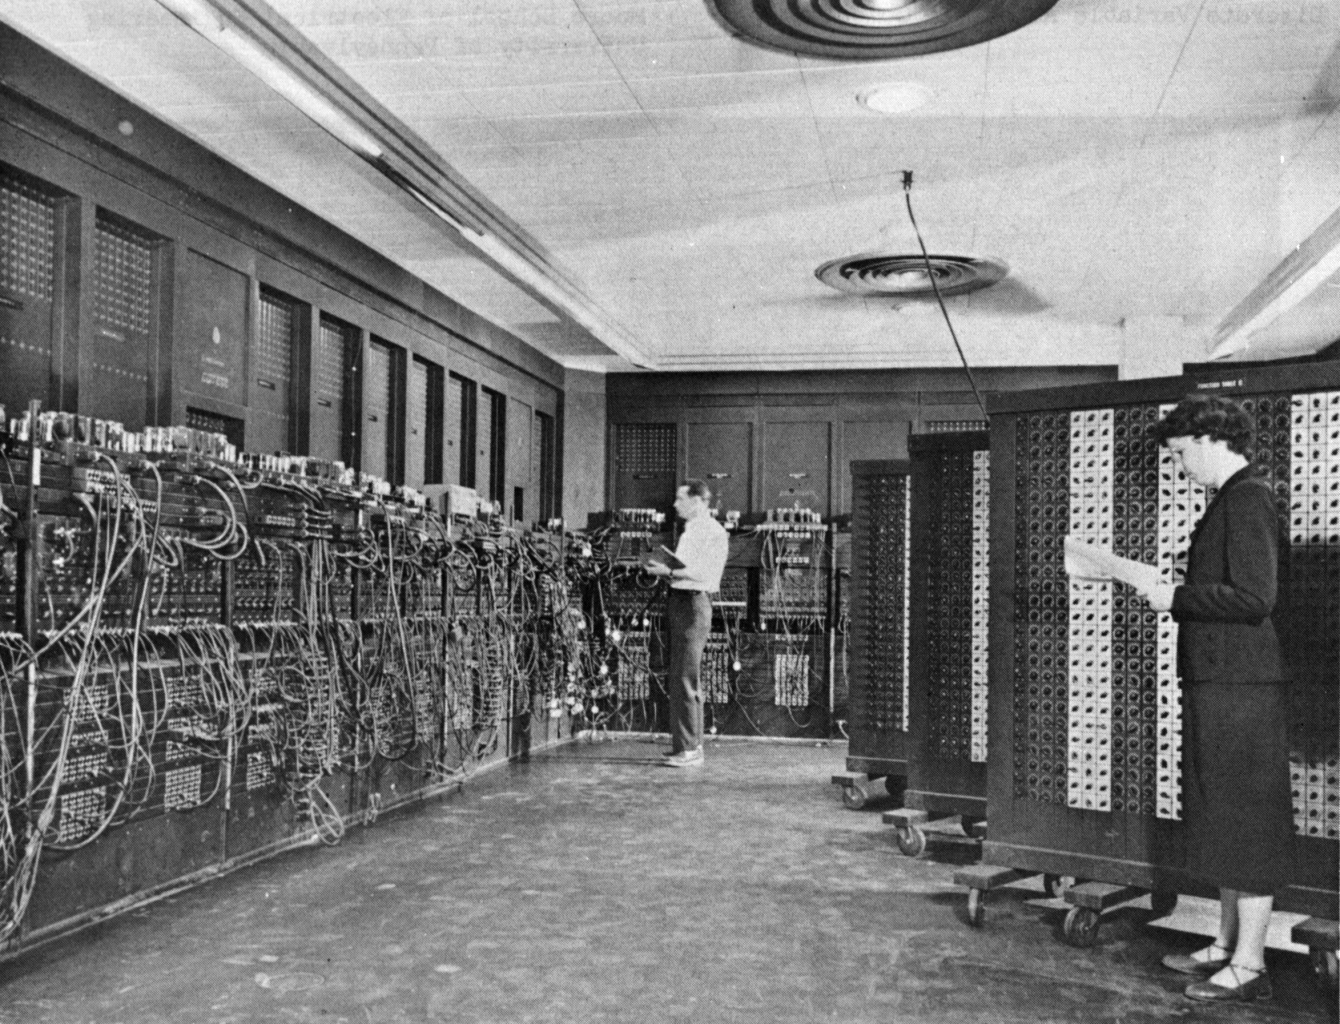
\includegraphics [width=.8\textwidth] {\inc/eniac}
	\\
	\creditphoto {U.S. Army} {domaine public}
    \end {center}

\end {frame}

\begin {frame} {Historique -- Les premiers ordinateurs}

    Sur ces ordinateurs~:

    \begin {itemize}
	\item programmer : câbler des connexions entre les unités

	\item résultats : à consulter sur des indicateurs lumineux

    \end {itemize}

    L'ordinateur~:
    \begin {itemize}
	\item est très onéreux (généralement un seul exemplaire)
	\item est très difficile à programmer (6 programmeuses à l'origine
	    sur l'ENIAC, la programmation dure plusieurs semaines)
	\item se programme par câblage physique
	\item n'exécute qu'un seul programme à la fois
	\item n'a pas ou peu de périphériques
    \end {itemize}

    \implique pas de système d'exploitation

\end {frame}


\begin {frame} {Historique -- Démarrage aux clefs}

    Étape suivante~:

    \begin {center}
	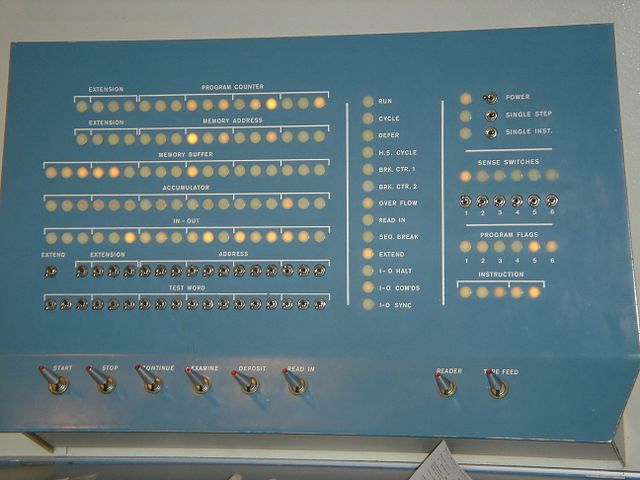
\includegraphics [width=.5\textwidth] {\inc/pdp1}
	\\
	\creditphoto {"PDP-1 control board" by fjarlq / Matt - http://www.flickr.com/photos/fjarlq/147938903/} {\ccby}
    \end {center}

    \begin {itemize}
	\item panneau de commande de l'ordinateur
	\item saisie du programme en mémoire avec des interrupteurs
	\item lancement du programme avec un interrupteur
	\item lecture du résultat avec les indicateurs lumineux
    \end {itemize}
    \implique pas de système d'exploitation

\end {frame}


\begin {frame} {Historique -- Carte perforée}

    La carte perforée (début des années 1950)

    \begin {minipage} [c] {.40\textwidth}
    \begin {center}
	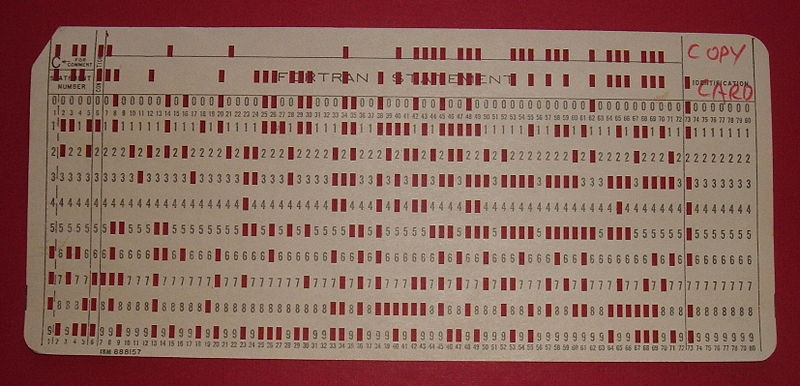
\includegraphics [width=\textwidth] {\inc/carte-perfo}
	\\
	\creditphoto {Arnold Reinhold} {\ccbysa}
    \end {center}
    \end {minipage}
    \hfill
    \begin {minipage} [c] {.58\textwidth}
    \begin {center}
	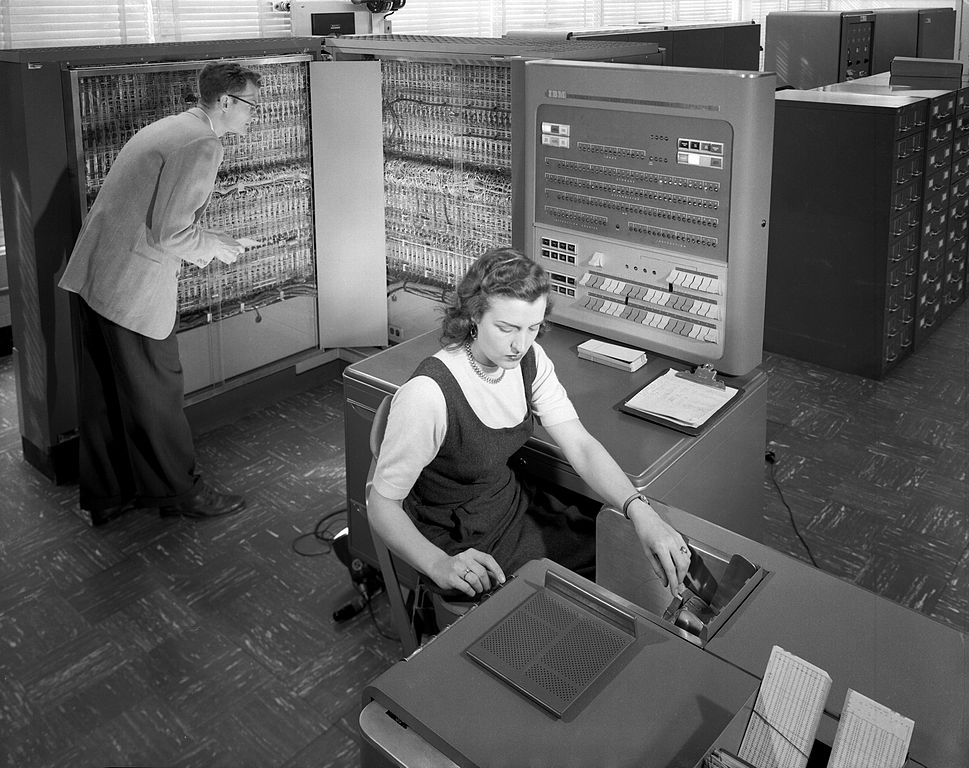
\includegraphics [width=\textwidth] {\inc/ibm704}
	\\
	\creditphoto {NASA (IBM 704)} {domaine public}
    \end {center}
    \end {minipage}

    \begin {itemize}
	\item périphérique d'entrée des programmes (et des données)
	\item programme en mémoire (morte) pour démarrer le lecteur,
	    stocker le programme en mémoire, et lancer son exécution
    \end {itemize}

\end {frame}

\begin {frame} {Historique -- Moniteur}

    Carte perforée \implique entrée automatisée des programmes

    \vspace* {3mm}

    Cependant :

    \begin {itemize}
	\item intervention d'un opérateur humain pour :
	    \begin {itemize}
		\item placer le bac de cartes dans le lecteur
		\item lancer la lecture
		\item attendre la fin du programme
		\item récupérer les résultats (sur l'imprimante)
	    \end {itemize}

	\item l'ordinateur est très onéreux : toute minute de calcul
	    perdue coûte cher !

    \end {itemize}

    D'où : programmes « \textbf {moniteurs} » résidant en mémoire

    \begin {itemize}
	\item toujours un seul programme à la fois
	\item automatisation du passage des différents programmes
	\item traitement par « lot » (de cartes) \implique
	    \textbf {batch processing}
	\item accès facilité aux périphériques
	\item premiers embryons de systèmes d'exploitation
    \end {itemize}

\end {frame}

\begin {frame} {Historique -- Spooling}
    Ordinateur onéreux \implique mieux le rentabiliser ?

    \begin {itemize}
	\item certains périphériques (lecteur de cartes perforées,
	    imprimante) sont lents

	    \includegraphics [width=.9\textwidth] {\inc/spool1}


	\item peut-on lancer un calcul pendant que les périphériques
	    lents travaillent ?

	    \includegraphics [width=.9\textwidth] {\inc/spool2}

    \end {itemize}

\end {frame}

\begin {frame} {Historique -- Spooling}
    Exemple~: IBM 7094 (1963)

    \begin {center}
	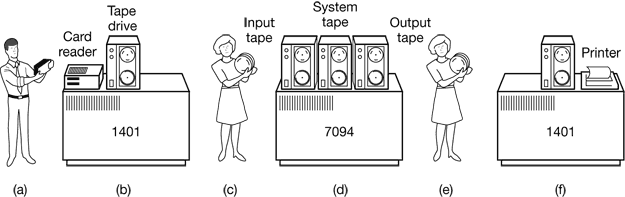
\includegraphics [width=.8\textwidth] {\inc/spool-tanenb}
	\\
	\credit {Extrait de Tanenbaum, A.S., Woodhull A.S.,
		« Operating Systems, Design and Implementation »,
		3rd ed, Pearson}
    \end {center}

    \begin {itemize}
	\item IBM 7094 : très onéreux
	\item IBM 1401 : peu coûteux (pour l'époque) \\
	    \implique dédié aux
	    transferts entre périphériques lents et bandes magnétiques
	    (rapides)
	\item transfert manuel des bandes \\
	    \implique évolution vers une connexion directe \\
	    \implique évolution vers des disques durs

    \end {itemize}
\end {frame}

\begin {frame} {Historique -- Spooling}
    En résumé :

    \begin {itemize}
	\item évolution vers des « périphériques » plus
	    « intelligents »
	\item fonctionnent en parallèle avec le processeur
	    central

    \end {itemize}

    \vspace* {3mm}

    \implique il faut maintenant tirer parti de ce parallélisme

    \begin {itemize}
	\item le moniteur doit gérer les ressources matérielles lentes
	    pour en exploiter le parallélisme
    \end {itemize}
\end {frame}

\begin {frame} {Historique -- Multi-programmation}
    Et lorsque le programme attend le résultat d'une entrée/sortie ?

    \begin {itemize}
	\item « démocratisation » des périphériques
	\item ex: stockage ou récupération d'une donnée temporaire
	    sur un périphérique (bande magnétique, disque dur, etc.)

	\item temps mort pour le processeur \\
	    \implique utiliser ce temps mort pour un autre programme

    \end {itemize}

    \vspace* {3mm}

    Introduction de la multi-programmation \implique \textbf {superviseur}
\end {frame}

\begin {frame} {Historique -- Multi-programmation}

    Le superviseur charge plusieurs programmes en mémoire~:
    \begin {itemize}

	\item lorsque le programme en cours demande une E/S, le
	    superviseur démarre le programme suivant
	\item lorsque le contrôleur d’E/S signale la fin de l’E/S,
	    le premier programme reprend son exécution
    \end {itemize}

    \vspace* {3mm}

    Exemple~: Atlas Supervisor de l'U. de Manchester (1962)
\end {frame}

\begin {frame} {Historique -- Multi-programmation}
    Questions posées par la multiprogrammation~:

    \begin {itemize}
	\item comment protéger les programmes les uns des autres ?
	    \\
	    \implique accès interdit aux variables d'un autre programme

	    \implique \textbf {unité de gestion mémoire} (composant matériel)

	\item comment le superviseur reprend le contrôle
	    lorsque le contrôleur d'E/S a terminé ?

	    \implique \textbf {mécanisme d'interruptions}
    \end {itemize}

\end {frame}

\begin {frame} {Historique -- Télétype}
    \begin {minipage} [c] {.40\textwidth}
    \begin {center}
	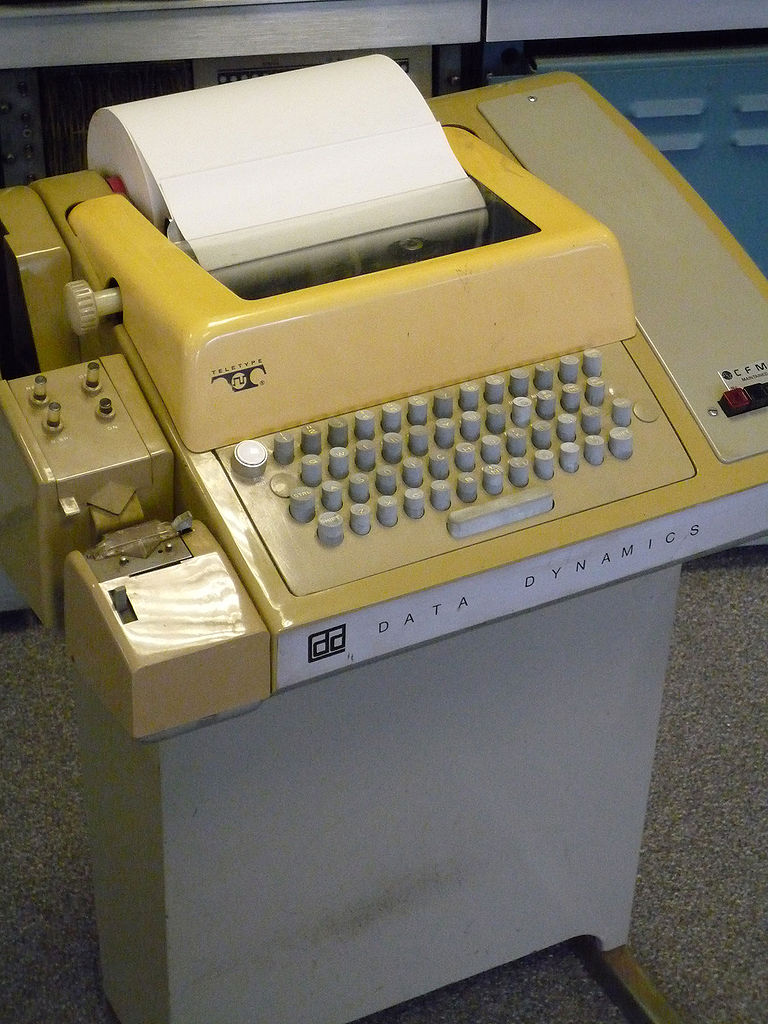
\includegraphics [width=\textwidth] {\inc/tty}
	\\
	\creditphoto {AlisonW} {\ccbysa}
    \end {center}
    \end {minipage}
    \hfill
    \begin {minipage} [c] {.58\textwidth}
	Ceci est une révolution !
	\begin {itemize}
	    \item changement fondamental dans l'interaction
		avec l'ordinateur
	    \item plus besoin d'attendre le passage du bac de
		cartes perforées sur l'ordinateur
	    \item commandes tapées au clavier \\
		\implique langage de commandes
	    \item résultat directement imprimé
	\end {itemize}
    \end {minipage}

\end {frame}

\begin {frame} {Historique -- Télétype}

    \begin {itemize}
	\item c'est un périphérique comme un autre...

	\item ... mais l'interaction modifie le besoin

	\item le superviseur lance des actions suite à des
	    commandes tapées à la console

	\item usage « interactif » $\neq$ usage « batch »

    \end {itemize}

\end {frame}

\begin {frame} {Historique -- Temps partagé}
    Connecter plusieurs terminaux à un même ordinateur :

    \begin {itemize}
	\item accueillir plusieurs utilisateurs
	\item mieux rentabiliser le coût d'un ordinateur
	\item connexion via une liaison série directe, ou via un modem
	\item donner à chacun l'impression d'avoir « son » ordinateur
	\item systèmes à temps partagé
    \end {itemize}

    Exemples~:
    \begin {itemize}
	\item CTSS (Compatible Time-Sharing System) : MIT (1961)
	    \\
	    IBM 7094 modifié par IBM, 32 utilisateurs maximum
	\item STSS (Stanford Time-Sharing System) : Stanford (1963)
	    \\
	    DEC PDP-1, 12 terminaux
    \end {itemize}
\end {frame}

\begin {frame} {Historique -- Temps partagé}
    Allouer le processeur pendant des petites portions de temps à
    chaque utilisateur~:

    \begin {itemize}
	\item quantum : durée fixée par le système (ex: 20 ms)
	\item pour un être humain, les programmes semblent tourner
	    en parallèle
    \end {itemize}


    \begin {center}
	\includegraphics [width=.9\textwidth] {\inc/quantum}
    \end {center}

\end {frame}

\begin {frame} {Historique -- Temps partagé}
    Questions posées par le temps partagé~:

    \begin {itemize}
	\item comment reprendre le contrôle à la fin de quantum ?
	    \\
	    \implique mécanisme d'\textbf {horloge} avec interruption

	\item comment gérer plusieurs utilisateurs ?
	    \\
	    \implique identité : validation et autorisations \\
	    \implique mécanismes logiciels

	\item comment éviter qu'un utilisateur outrepasse ses droits ?
	    \\
	    \implique \textbf {modes d'exécution} privilégié et non
		privilégié \\
	    \implique quelques instructions interdites en mode non
		privilégié

	    \vspace* {1mm}

	    Exemple~:
	    \begin {itemize}
		\item accès au disque : réservé au mode
		    privilégié
		\item programmes utilisateurs : exécutés
		    en mode non privilégié
		    \\
		    \implique passage par le système pour
		    accéder aux fichiers
	    \end {itemize}

    \end {itemize}

\end {frame}

\begin {frame} {Historique -- Appel système}
    Lorsqu'un programme souhaite effectuer (par exemple) un accès
    disque, il fait un \textbf {appel système} :

    \begin {itemize}
	\item instruction spéciale (TRAP, SVC, INT, etc. suivant le
	    processeur)

	\item provoque (entre autres) :
	    \begin {itemize}
		\item basculement en mode privilégié
		\item déroutement du programme vers une adresse spécifique
	    \end {itemize}

	\item adresse spécifique = système d'exploitation
	\item \textbf {vérification} des paramètres, des droits, etc.
	    \\
	    \implique pour éviter qu'un utilisateur outrepasse ses droits
	\item réalisation de l'action demandée par l'appel système

    \end {itemize}

\end {frame}

\begin {frame} {Historique -- Temps partagé}

    Début des années 1970 : terminaux à écran cathodique

    \begin {center}
	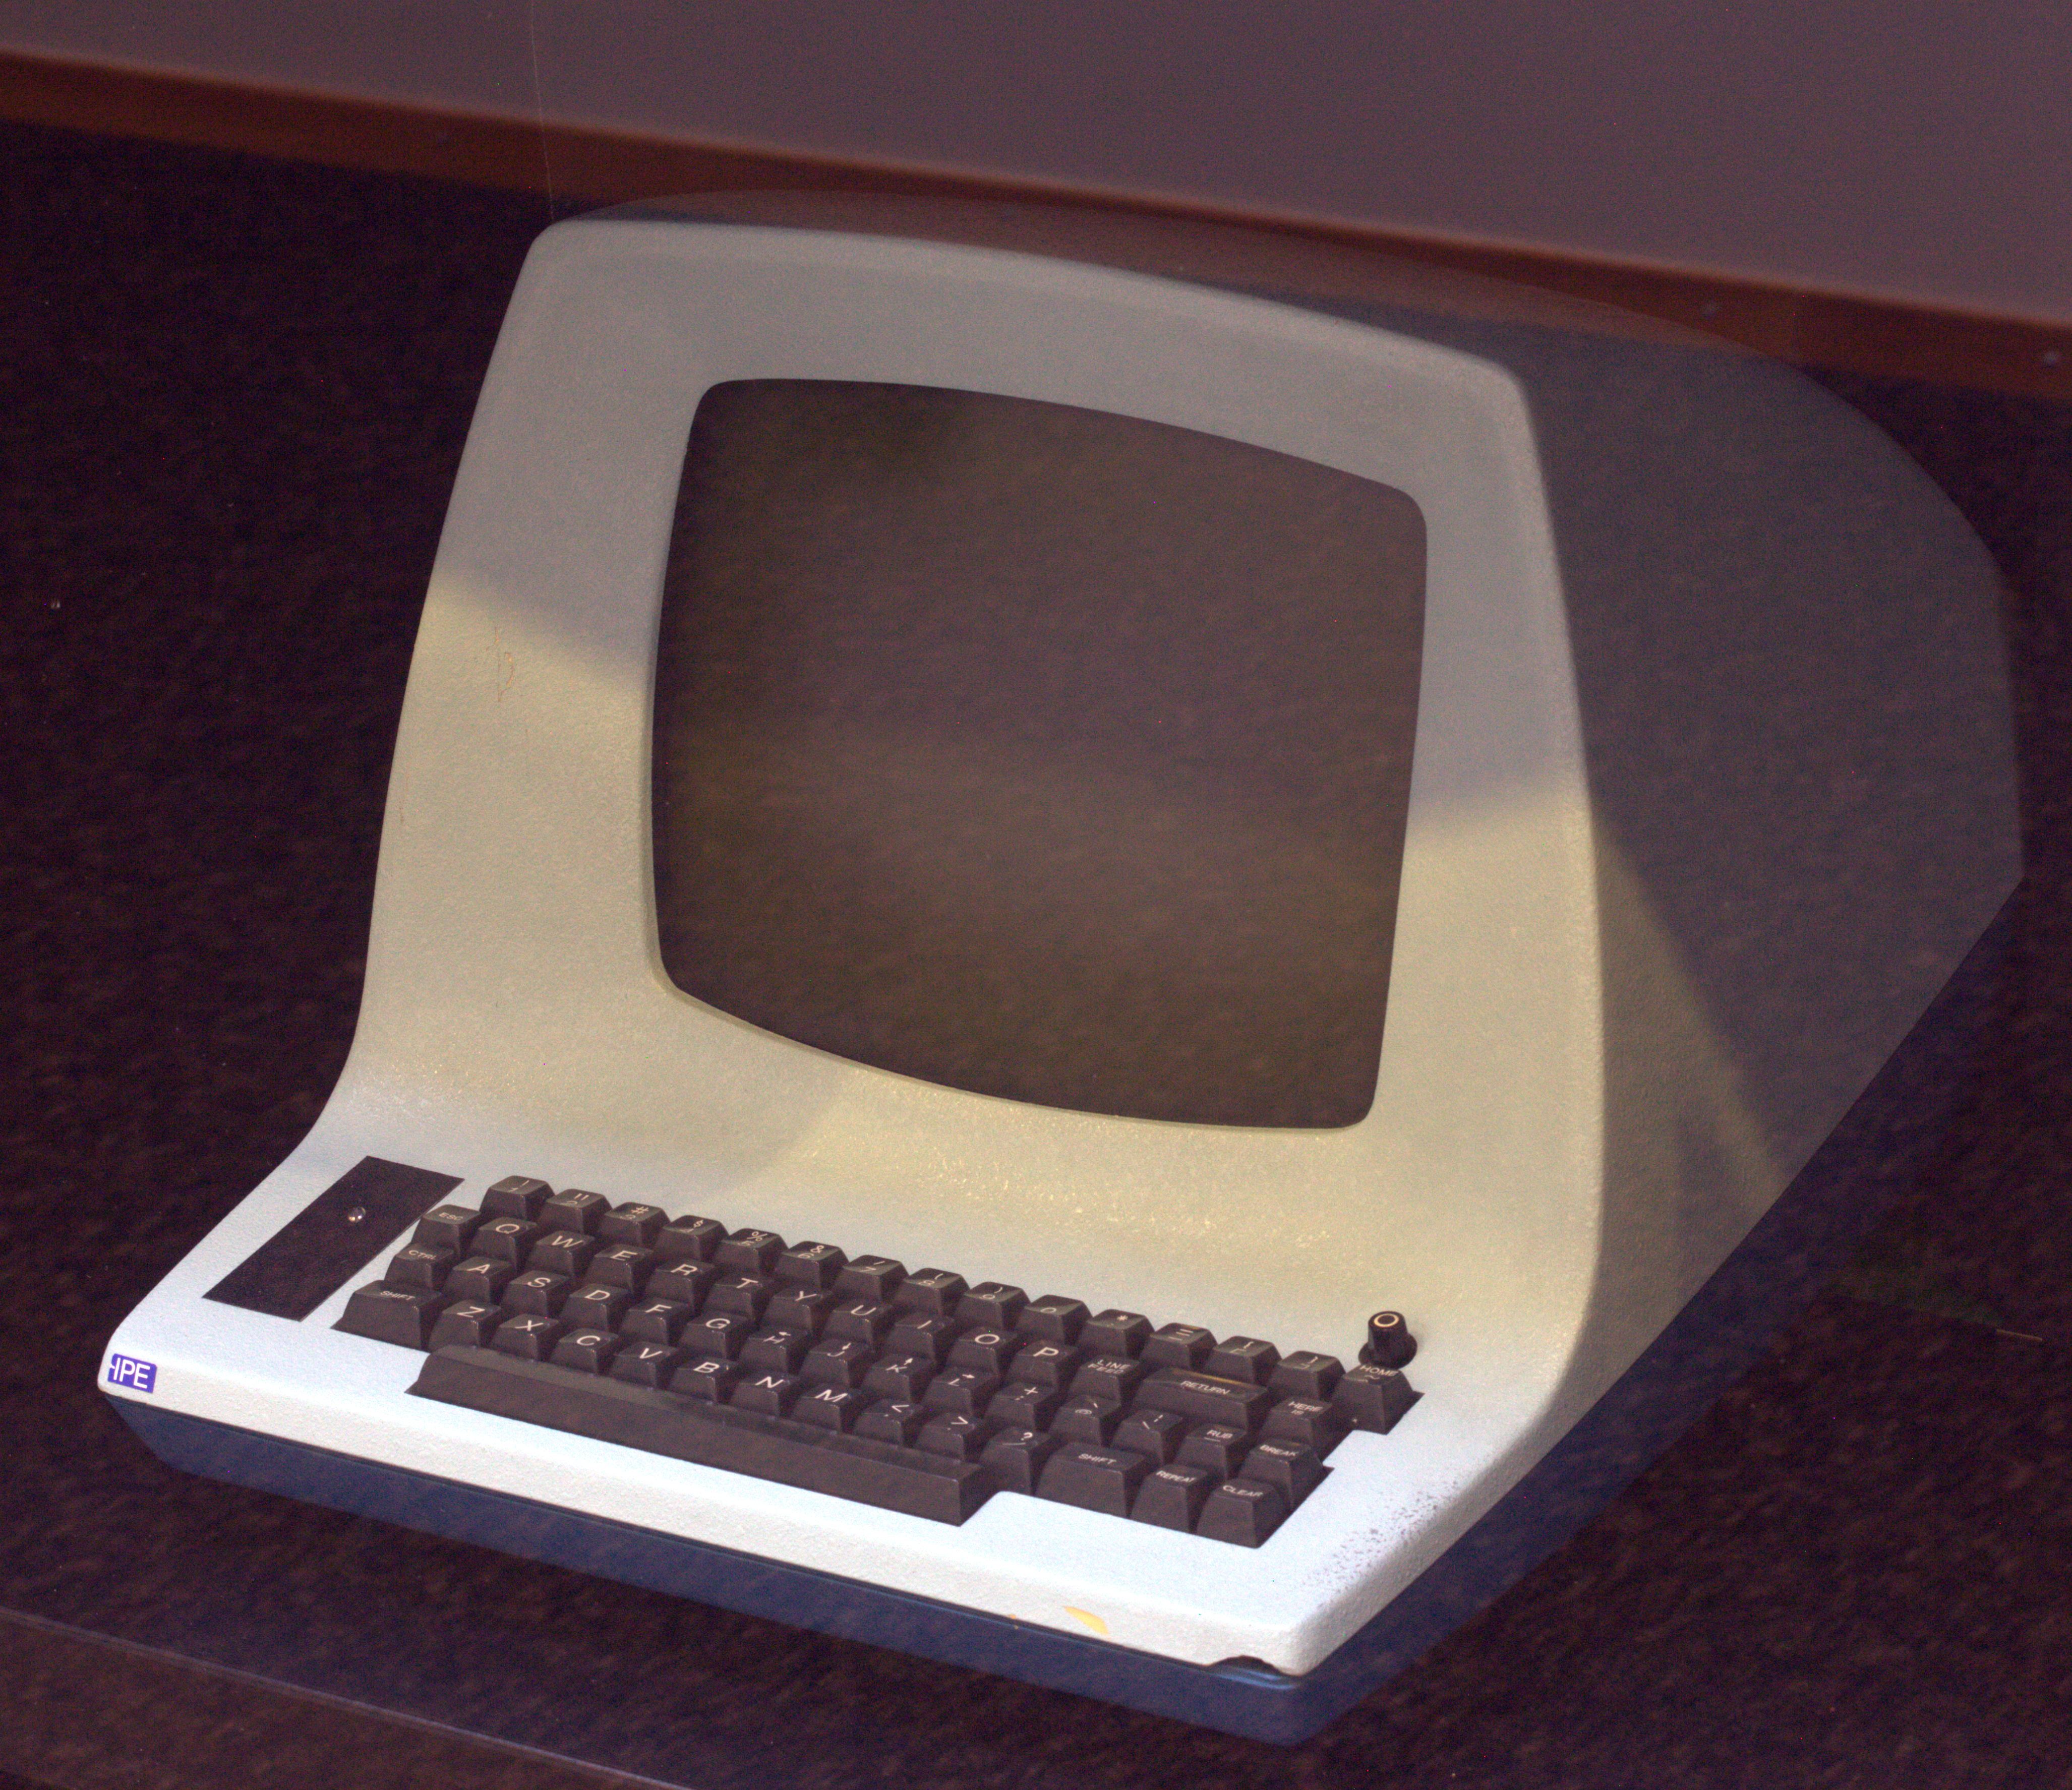
\includegraphics [width=.4\textwidth] {\inc/term-adm3a}
	\\
	\creditphoto {"Lear Siegler ADM-3A-IMG 1508" by Photograph by
	Rama} {\ccbysa}
    \end {center}

    \vspace* {3mm}

    Âge d'or des « mainframes »

    \implique stabilisation des systèmes d'exploitation autour des
    concepts vus précédemment

\end {frame}

\begin {frame} {Bilan}
    Fonctionnalités offertes par un système d'exploitation

    \begin {itemize}
	\item rentabiliser l'usage de l'ordinateur
	    \\
	    \implique utiliser tous les temps morts
	\item partager un ordinateur entre plusieurs utilisateurs
	    \\
	    \implique partager équitablement les ressources matérielles

	\item faciliter l'accès aux périphériques
	    \\
	    \implique offrir une interface avec le matériel
	    \\
	    \implique pour tirer parti du parallélisme des périphériques

	\item permettre à des utilisateurs d'éditer, développer,
	    lancer des programmes
    \end {itemize}

    ... le tout en offrant les garanties de sécurité nécessaires
\end {frame}

%%%%%%%%%%%%%%%%%%%%%%%%%%%%%%%%%%%%%%%%%%%%%%%%%%%%%%%%%%%%%%%%%%%%%%%%%%%%%%
% Le noyau
%%%%%%%%%%%%%%%%%%%%%%%%%%%%%%%%%%%%%%%%%%%%%%%%%%%%%%%%%%%%%%%%%%%%%%%%%%%%%%

\titreB {Le noyau}

\begin {frame} {Continuons l'historique}

    Systèmes d'exploitation marquants~:

    \begin {itemize}
	\item Burroughs MCP (1961)
	    \begin {itemize}
		\item conçu pour l'ordinateur Burroughs B5000
		\item premier SE programmé en \textbf {langage de
		    haut niveau}
		\item beaucoup d'éléments innovants (multiprocesseurs,
		    mémoire virtuelle)
	    \end {itemize}
	\item IBM OS/360 (1964)
	    \begin {itemize}
		\item SE « universel » pour les ordinateurs IBM System/360
		\item énorme (des dizaines de millions de lignes d'assembleur)
		\item \textbf {complexe}, beaucoup de retards
		\item F. Brooks « The Mythical Man-Month »
	    \end {itemize}
	\item CTSS (\textbf {MIT}, 1961)
	    \begin {itemize}
		\item premier système multi-utilisateurs
		\item IBM 7094 modifié (2 exemplaires)
	    \end {itemize}
    \end {itemize}

\end {frame}

\begin {frame} {Multics}

    \begin {itemize}
	\item Multics (MULtiplexed Information and Computing Service)
	    \ctableau {\fD} {|l|l|} {
		1963 & spécification (MIT) \\
		1964 & démarrage du projet \\
		1964 & General Electric + Bell Labs rejoignent le MIT \\
		1968 & première version « self-hosting » \\
		1969 & \textbf {Bell Labs} se retirent du projet \\
		1973 & annonce commerciale \\
		1985 & fin du développement \\
		2000 & fermeture du dernier site (Min Défense Canada) \\
	    }

	    \begin {itemize}
		\item Système très ambitieux
		\begin {itemize}
		    \item écrit en langage de haut niveau (PL/1)
		    \item accès uniforme à la mémoire et aux fichiers
		    \item système de fichiers hiérarchique
		    \item édition de liens dynamique
		    \item reconfiguration matérielle dynamique
		    \item processus « démons »
		    \item sécurité (certification B2 en 1985)
		\end {itemize}
		\item 84 sites au total (dont 31 universités/centres français)
	    \end {itemize}
    \end {itemize}

\end {frame}

\begin {frame} {Unix}

    \begin {itemize}
	\item Unix
	    \ctableau {\fD\rowcolors {2} {bleufonce} {bleuclair}} {|l|l|} {
		\rca
		1969 & Bell Labs se retirent du projet Multics \\
		      & récupération d'un PDP-7, écriture en assembleur \\
		1971 & achat PDP-11/20 en échange d'un formateur de texte \\
		1972 & création du langage C et réécriture d'Unix en C \\
		1973 & premières diffusions \\
		1979 & Unix v7 (environ 10 000 lignes de C et un peu
		    d'assembleur) \\
		1980 & distribution 4BSD \\
		1992 & procès AT\&T vs BSDi vs Berkeley (fin en 1994) \\
	    }

	    \begin {itemize}
		\item Beaucoup d'idées novatrices
		    \begin {itemize}
			\item simple
			\item écrit en langage C
			\item séparation nette \textbf {noyau} / utilitaires
			    (ou applications)
			\item tout est fichier
			\item pas de structure interne des fichiers
			\item interface utilisateur simple (minimaliste)
			\item philosophie Unix (kiss : « keep it simple, stupid »)
			\item portable
		    \end {itemize}
	    \end {itemize}
	    
    \end {itemize}

\end {frame}

\begin {frame} {Le noyau}
    Philosophie Unix \implique approche minimaliste,
    à l'opposé des systèmes d'exploitation précédents

    \vspace* {3mm}

    Le noyau a deux objectifs fondamentaux~:
    \begin {itemize}
	\item \textbf {partager équitablement les ressources}
	\item \textbf {garantir la sécurité des données}
    \end {itemize}

\end {frame}

\begin {frame} {Le noyau}
    Partager équitablement les ressources~:

    \begin {itemize}
	\item mémoire vive
	\item temps processeur
	\item carte réseau
	\item espace disque
	\item accès aux disques
	\item etc.
    \end {itemize}
\end {frame}

\begin {frame} {Le noyau}
    Garantir la sécurité des données

    \begin {itemize}
	\item un processus ne doit pas accéder aux données d'un autre
	    processus (sauf si autorisé)

	\item un utilisateur ne doit pas accéder à un fichier non autorisé

	\item un utilisateur ne doit pas terminer un processus d'un
	    autre utilisateur

	\item etc.

    \end {itemize}
\end {frame}

\begin {frame} {Le noyau}

    Pour atteindre les deux objectifs fondamentaux :

    \begin {itemize}
	\item le \textbf {noyau} s'exécute en \textbf {mode privilégié}
	    \\
	    \implique il a accès à toutes les ressources matérielles

	\item les programmes (applications) s'exécutent, dans le
	    contexte de \textbf {processus}, en \textbf {mode non
	    privilégié}
	    \\
	    \implique appels au noyau pour exécuter certaines opérations

    \end {itemize}

    \vspace* {3mm}

    Les appels au noyau sont les \textbf {primitives systèmes}

    \begin {itemize}
	\item Interface de programmation du noyau
	    \\
	    \textit {Application Programming Interface} (API)
	\item Forme : appels de fonction en C
	\item Exemple :
	    \\
	    \code {int open (const char *path, int flag, mode\_t mode)}
    \end {itemize}


\end {frame}

\begin {frame} {Le noyau}
    \begin {center}
	\includegraphics [width=.7\textwidth] {\inc/noyau}
    \end {center}
\end {frame}

\begin {frame} {Le noyau}
    Définition :

    \begin {quote}
	Le noyau est constitué de l'ensemble minimum des primitives
	systèmes nécessaires pour atteindre les deux objectifs
	fondamentaux

    \end {quote}

\end {frame}

\begin {frame} {Le noyau}
    \begin {itemize}
	\item Démarrage de l'ordinateur : noyau installé
	    en mémoire \\
	    \implique il y restera jusqu'à la fin (redémarrage,
	    arrêt, ou crash)

	\item Le noyau s'exécute en mode privilégié

	    \begin {itemize}
		\item code sensible
		\item difficile à développer, à mettre au point
		\item plus il est petit, mieux c'est
		\item tout ce qui peut être mis ailleurs doit l'être
		    \\
		    \vspace* {0.8mm}
		    Exemple :
		    \begin {itemize}
			\item pour le noyau, un utilisateur = un nombre
			    entier
			\item \code {ls -l} affiche des noms de login
			\item \implique la conversion
			    « entier $\leftrightarrow$ nom » est
			    effectuée par \code {ls}

		    \end {itemize}
	    \end {itemize}

	\item Mise en évidence du concept de noyau \\
	    \implique apport majeur d'Unix

    \end {itemize}

\end {frame}

\begin {frame} {Le noyau}
    Quelles fonctions doivent être des primitives systèmes ?

    \begin {itemize}
	\item un processus ne doit pas avoir le droit d'accéder
	    directement au disque (violation du deuxième objectif)
	    \\
	    \implique il faut que le noyau présente une abstraction avec
	    des droits : système de fichiers, propriétaire,
	    droits d'accès \\
	    \implique accès au disque par l'intermédiaire de cette
	    abstraction
	    \\
	    \implique \code {open} est une primitive système

	\item lire l'heure courante \implique accès à un périphérique
	    \\
	    \implique \code {time} est une primitive système

    \end {itemize}
\end {frame}

\begin {frame} {Le noyau}
    Quelles fonctions doivent être des primitives systèmes ?

    \begin {itemize}
	\item \code {strlen} calcule un nombre d'octets en lisant
	    dans la mémoire du processus courant (donc autorisé)
	    \\
	    \implique \code {strlen} n'est donc pas une primitive système

	    \vspace* {1mm}

	    Comme elle est utile, on la met\footnote {Ou plus exactement
	    son code compilé.} dans une \textbf {bibliothèque} une
	    fois pour toutes, pour éviter d'avoir à la reprogrammer
	    à chaque fois

	\item \code {getlogin} renvoie le nom de login de l'utilisateur
	    \\
	    \implique cette fonction récupère le numéro de
	    l'utilisateur avec une primitive système, puis convertit ce
	    numéro en nom en parcourant le fichier \code {/etc/passwd}
	    (ou en utilisant une base externe LDAP dans le cas de turing)
	    \\
	    \implique \code {getlogin} n'est pas une primitive système

    \end {itemize}
\end {frame}

\begin {frame} {Interface utilisateur}
    \ctableau {\fD} {|l|l|l|} {
	Date & \multicolumn {1} {c|} {Stations de travail}
		& \multicolumn {1} {c|} {Ordinateurs personnels}
	    \\ \hline
	1968 & \multicolumn {2} {l|} {Prototype de souris par
		Douglas Englebart (Stanfort Research Institute)} \\
	1973 & Alto (Xerox) & \\
	1981 & Display Manager (Apollo Computer) & \\
	1983 & W Window System (Stanford) & Lisa (Apple) \\
	1984 & X Window System (MIT) & \\
	1985 & HP Windows (HP),	& Amiga Workbench (Commodore), \\
	     & Sunview (Sun)	& Windows (Microsoft), etc \\
    }

    La gestion d'une interface utilisateur « graphique » n'est pas
    du ressort du noyau :
    \begin {itemize}
	\item Souris, écran graphique, écran tactile (tablette, etc.) \\
	    \implique périphériques gérés par le noyau
	\item Système de fenêtrage \\
	    \implique applications
    \end {itemize}
\end {frame}

\begin {frame} {Qu'est-ce qu'un système d'exploitation ?}
    Retour sur notre interrogation du début :
    \begin {itemize}
	\item Unix (l'original, puis les *BSD) : noyau + applications
	\item Linux est un noyau
	    \begin {itemize}
		\item des organisations (bénévoles ou commerciales) ont
		    réuni des applications, les ont compilées et ont
		    diffusé, avec le noyau, des \textbf {distributions}
		    prêtes à l'emploi

	    \end {itemize}
	\item Windows : noyau + applications
	\item Android, iOS : noyau (avec support de périphériques tactiles,
	    audio, GSM, GPS, etc.) + applications
	\item box Internet, montre connectée, voiture, etc. : noyau
	    +  applications spécifiques
	\item etc.
    \end {itemize}
\end {frame}

\begin {frame} {Quelques systèmes atypiques}
    \begin {itemize}
	\item systèmes temps réel
	\item systèmes contraints (ex: Internet des Objets)
    \end {itemize}
\end {frame}

\begin {frame} {Bilan}
    \begin {itemize}
	\item Depuis Unix : distinction entre noyau et reste du système
	    d'exploitation

	\item Objet de cette UE : comprendre le fonctionnement d'un noyau
	    de système d'exploitation

    \end {itemize}

\end {frame}

%%%%%%%%%%%%%%%%%%%%%%%%%%%%%%%%%%%%%%%%%%%%%%%%%%%%%%%%%%%%%%%%%%%%%%%%%%%%%%
% POSIX
%%%%%%%%%%%%%%%%%%%%%%%%%%%%%%%%%%%%%%%%%%%%%%%%%%%%%%%%%%%%%%%%%%%%%%%%%%%%%%

\titreB {POSIX}

\begin {frame} {Interface des primitives systèmes}
    Primitives systèmes = ensemble de fonctions (appelables en C)
    pour accéder aux services offerts par le noyau

    \begin {itemize}
	\item À l'origine (Unix v6, 1975) : 43 primitives
	\item Évolutions ultérieures (années 1980) :
	    \begin {itemize}
		\item Bell Labs, AT\&T
		\item U. de Berkeley
		\item Essor commercial
	    \end {itemize}
	\item Résultat
	    \begin {itemize}
		\item de nombreuses divergences \implique incompatibilités
		\item les programmes ne sont plus portables
		\item les utilisateurs ne sont pas contents
	    \end {itemize}
	\item Il faut normaliser l'existant \implique POSIX
    \end {itemize}

\end {frame}

\begin {frame} {POSIX}

    Comité POSIX de l’IEEE
    \begin {itemize}
	\item IEEE = Institute of Electrical and Electronics Engineers
	    \\
	    (association américaine, rédige des textes normatifs)
	\item POSIX = Portable Operating System Interface
	\item Norme IEEE : IEEE Std 1003.*
	\item Norme internationale : ISO/IEC 9945
	\item Première version : 1988
	\item Version actuelle : 2013
    \end {itemize}

    \vspace* {3mm}

    Impact majeur \implique aucun système d'exploitation ne peut
    se permettre de ne pas être compatible POSIX
\end {frame}

\begin {frame} {POSIX}

    POSIX normalise beaucoup de choses :

    \begin {itemize}
	\item des primitives systèmes et des fonctions de bibliothèque
	\item des commandes (\code {sh}, \code {ls}, \code {tr}, etc.)
	\item des extensions (temps réel, threads, sémaphores, etc.)
    \end {itemize}

    \vspace* {3mm}

    POSIX ne normalise pas tout :
    \begin {itemize}
	\item une implémentation peut avoir ses propres extensions \\
	    \implique non normalisées \implique non portables
	\item Exemple avec \code {ls} :
	    \begin {itemize}
		\item POSIX 2013 : 23 options (c'est beaucoup...) \\
		\item GNU (Linux) : 58 options (c'est trop !) \\
	    \end {itemize}
	\item programmer portable \implique respecter POSIX
	\item utiliser la notice fournie en cours

    \end {itemize}

\end {frame}

\begin {frame} {POSIX}

    POSIX ne fait pas de distinction entre primitive système et fonction
    de bibliothèque :

    \begin {itemize}
	\item laisser de la liberté pour les implémentations
	\item distinction parfois mince
	    \begin {itemize}
		\item Exemple : 6 fonctions pour exécuter un programme
		    (\code {execv}, \code {execl}, \code {execvp},
		    \code {execlp}, \code {execve} et \code {execle}),
		    une seule est une primitive, les 5 autres sont des
		    fonctions de bibliothèque
	    \end {itemize}
    \end {itemize}
\end {frame}

\begin {frame} {POSIX}
    Principes généraux

    \begin {itemize}
	\item Types POSIX
	\item Constantes
	\item Gestion des erreurs
	\item Paramètres de type « pointeur »
    \end {itemize}
\end {frame}

\begin {frame} {POSIX -- Types}
    \begin {itemize}
	\item Le noyau Unix manipulait des objets grâce à des entiers

	    \vspace* {1mm}
	    Problème : portabilité (16/32/64 bits ? implémentations ?)

	\item POSIX a introduit de nouveaux types (avec \code {typedef})
	    \\
	    \implique masquer le détail d'implémentation \\
	    \implique portabilité des programmes

	    \vspace* {1mm}
	    Quelques exemples :

	    \ctableau {\fC} {|l|l|} {
		\code {uid\_t} & numéro d'utilisateur \\
		\code {gid\_t} & numéro de groupe \\
		\code {pid\_t} & numéro de processus \\
		\code {mode\_t} & permissions \\
		\code {time\_t} & heure courante \\
		\code {size\_t} & taille, résultat de sizeof (définie par ISO C) \\
	    }

	    Définitions des types : fichiers d'inclusion
    \end {itemize}

\end {frame}

\begin {frame} {POSIX -- Constantes}
    \begin {itemize}
	\item Certaines primitives nécessitent de spécifier une opération

	\item Exemple~:
	    \ctableau {\fC} {|l|l|} {
		\code {r = access ("toto", 0)}
		    & le fichier existe-t'il ? \\
		\code {r = access ("toto", 1)}
		    & puis-je exécuter le fichier ? \\
		\code {r = access ("toto", 2)}
		    & puis-je modifier le fichier ? \\
		\code {r = access ("toto", 4)}
		    & puis-je lire le fichier ? \\
	    }

	    \vspace* {3mm}

	\item Il faut se rappeler des valeurs et de leur signification
    \end {itemize}

\end {frame}

\begin {frame} {POSIX -- Constantes}
    \begin {itemize}

	\item Définition de constantes (dans les fichiers d'inclusion)

	    Fichier \code {unistd.h} :
	    \lstinputlisting [basicstyle=\fD\lstmonstyle] {\inc/unistd.h}

	\item L'exemple précédent devient :
	    \ctableau {\fC} {|l|l|} {
		\code {r = access ("toto", F\_OK)}
		    & le fichier existe-t'il ? \\
		\code {r = access ("toto", X\_OK)}
		    & puis-je exécuter le fichier ? \\
		\code {r = access ("toto", W\_OK)}
		    & puis-je modifier le fichier ? \\
		\code {r = access ("toto", R\_OK)}
		    & puis-je lire le fichier ? \\
	    }
	    \vspace* {2mm}

	\item Utiliser les constantes rend les programmes plus lisibles

	\item Parfois, les constantes sont moins pratiques (permissions)
	    ou peu répandues

    \end {itemize}

\end {frame}

\begin {frame} {POSIX -- Constantes}
    Certaines constantes ne sont pas constantes...

    \begin {itemize}
	\item arguments sémantiques des primitives : fichiers d'inclusion
	    \begin {center}
		\fE
		Exemples~:
		\tableau {} {|l|l|l|} {
		    \code {R\_OK}
			& test en lecture pour \code {access}
			& \code {unicode.h}
			\\
		    \code {O\_WRONLY}
			& ouverture en écriture pour \code {open}
			& \code {fcntl.h}
			\\
		    \code {S\_IFDIR}
			& type de fichier « répertoire »
			& \code {sys/stat.h}
			\\
		    ... & &
			\\
		}
	    \end {center}

	\item limites arbitraires : \code {limits.h}
	    \begin {center}
		\fE
		Exemples~:
		\tableau {} {|l|l|} {
		    \code {PATH\_MAX}
			& taille maximum d'un chemin complet
			\\
		    \code {LOGIN\_NAME\_MAX}
			& taille maximum d'un nom de login
			\\
		    \code {CHILD\_MAX}
			& nombre maximum de processus fils
			\\
		}
	    \end {center}

	\item limites dépendant de la configuration du système \\
	    \code {long sysconf (int paramètre})
	    \begin {center}
		\fE
		Exemples~:
		\tableau {} {|l|l|} {
		    \code {\_SC\_LOGIN\_NAME\_MAX}
			& longueur maxium des noms d'utilisateur
			\\
		    \code {\_SC\_OPEN\_MAX}
			& nombre maximum d'ouvertures de fichier
			\\
		    \code {\_SC\_CHILD\_MAX}
			& nombre maximum de processus fils
			\\
		}
	    \end {center}

	\item limites dépendant du système de fichiers \\
	    \code {long pathconf (const char *chemin, int paramètre})
	    \begin {center}
		\fE
		Exemples~:
		\tableau {} {|l|l|} {
		    \code {\_PC\_LINK\_MAX}
			& nombre maximum de liens sur un fichier
			\\
		    \code {\_PC\_NAME\_MAX}
			& taille maximum d'un nom de fichier
			\\
		    \code {\_PC\_PATH\_MAX}
			& taille maximum d'un chemin complet
			\\
		}
	    \end {center}

    \end {itemize}
\end {frame}

\begin {frame} {POSIX -- Gestion des erreurs}
    En cas d'erreur, les primitives :
    \begin {itemize}
	\item renvoient -1 en cas d'erreur
	    \begin {itemize}
		\item ... sauf pour quelques très rares exceptions
	    \end {itemize}

	\item placent dans la variable \code {errno} un code reflétant l'erreur

    \end {itemize}

    \vspace* {3mm}

    Fichier \code {errno.h} :
    \lstinputlisting [basicstyle=\fD\lstmonstyle] {\inc/errno.h}

    \vspace* {3mm}

    Description de toutes les erreurs possibles pour une primitive \\
    \implique consulter POSIX ou le \code {man} de la primitive
\end {frame}

\begin {frame} {POSIX -- Gestion des erreurs}
    Exemple d'utilisation (laborieux) :

    \lstinputlisting [basicstyle=\fD\lstmonstyle] {\inc/ex-errno1.c}
\end {frame}

\begin {frame} {POSIX -- Gestion des erreurs}
    Mieux : mettre l'affichage dans une fonction

    \lstinputlisting [basicstyle=\fD\lstmonstyle] {\inc/perror.c}

    Très utile \implique bibliothèque standard :
    \begin {itemize}
	\item \code {void perror (const char *msg) ;}
	\item \code {char *strerror (int numerr) ;}
    \end {itemize}
\end {frame}

\begin {frame} {POSIX -- Gestion des erreurs}
    Exemple d'utilisation (final) :

    \lstinputlisting [basicstyle=\fD\lstmonstyle] {\inc/ex-errno2.c}
\end {frame}

\begin {frame} {POSIX -- Gestion des erreurs}
    \begin {block} {\casseroler {Recommandations}}
    \begin {itemize}
	\item \alert {toujours vérifier} les retours de primitives
	\item \alert {afficher} la raison des erreurs
    \end {itemize}
    \end {block}

    \lstinputlisting [basicstyle=\fD\lstmonstyle] {\inc/ex-errno3.c}
\end {frame}

\begin {frame} {POSIX -- Paramètres de type « pointeur »}

    Certaines primitives retournent des résultats plus complexes
    qu'un simple entier

    \begin {itemize}
	\item Paramètre de type pointeur (sur un objet à remplir)
	\item Exemples :
	    \begin {itemize}
		\item \code {int stat (const char *path,
				\alert {struct stat *stbuf})}
		    \\
		    Retourne dans l'emplacement repéré par \code
		    {\alert {stbuf}} les attributs du fichier
		\item \code {pid\_t wait (\alert {int *status})}
		    \\
		    Place dans l'emplacement repéré par \code {\alert
		    {status}} des informations sur la terminaison du
		    processus
		\item etc.
	    \end {itemize}

	\item L'emplacement mémoire pointé \textbf {doit exister} !
    \end {itemize}
\end {frame}

\begin {frame} {POSIX -- Paramètres de type « pointeur »}
    Exemples d'utilisation~:

    \ctableau {\fC} {|p{.49\textwidth}|p{.49\textwidth}|} {
	\multicolumn {1} {|c|} {\textbf {Correct}}
	    & \multicolumn {1} {c|} {\textbf {\alert {Faux}}}
	    \\ \hline
	\lstinputlisting [basicstyle=\fE\lstmonstyle] {\inc/ex-ptr-ok.c}
	    &
	    \lstinputlisting [basicstyle=\fE\lstmonstyle] {\inc/ex-ptr-bad.c}
	    \\
	La variable \code {stbuf} existe, on passe son adresse
	    & La variable \code {stbuf} est un pointeur non initialisé,
		le noyau va écrire le résultat quelque part (où ?) en
		mémoire
	    \\
    }

\end {frame}

\def\inc{inc2-file}

\titreA {Gestion des fichiers}

%%%%%%%%%%%%%%%%%%%%%%%%%%%%%%%%%%%%%%%%%%%%%%%%%%%%%%%%%%%%%%%%%%%%%%%%%%%%%%
% Accès aux fichiers
%%%%%%%%%%%%%%%%%%%%%%%%%%%%%%%%%%%%%%%%%%%%%%%%%%%%%%%%%%%%%%%%%%%%%%%%%%%%%%

\titreB {Accès aux fichiers}

\begin {frame} {Accès aux fichiers}
    Un fichier :
    \begin {itemize}
	\item a un nom (en fait, plusieurs...)
	\item est accessible via un chemin (absolu, relatif)
	\item possède des attributs :
	    \begin {itemize}
		\item type
		\item propriétaire, groupe, permissions
		\item taille
		\item dates
		    \begin {itemize}
			\item de dernière modification des données
			\item date de dernière modification des attributs
			\item date de dernier accès
		    \end {itemize}
		\item emplacement des données sur le disque
	    \end {itemize}
	\item 2 types de fichiers
	    \begin {itemize}
		\item fichiers « réguliers »
		\item répertoires
		\item ... en réalité, il y en a d'autres (plus tard...)
	    \end {itemize}
    \end {itemize}
\end {frame}

\begin {frame} {Accès aux fichiers}
    Un fichier a une structure simple : suite linéaire d'octets
    \begin {center}
	\includegraphics [width=.6\linewidth] {\inc/str-fich}
    \end {center}

    \begin {itemize}
	\item innovation d'Unix
	    \begin {itemize}
		\item dans les systèmes antérieurs : les fichiers avaient
		    un type (texte, base de données, etc.)
		\item pas de type \implique simplification du noyau
	    \end {itemize}

	\item la structure dépend de l'application qui accède au fichier

	    \begin {itemize}
		\item texte : suite de caractères séparés par
		    \code {\textbackslash n}
		    (octet 10)
		\item binaire exécutable : contient un en-tête qui
		    décrit les différentes parties (code, données,
		    infos de debug, etc.)
		\item document LibreOffice : cf application LibreOffice
		\item etc.
	    \end {itemize}

	\item notion de « \textit {magic number} »
	    \begin {itemize}
		\item suite d'octets au début d'un fichier pour l'identifier
		\item ex: \code {\#!} (script), \code {\%PDF} (fichier PDF),
		    \code {0xffd8} (JPEG), etc.
		\item commande \code {file}
	    \end {itemize}
    \end {itemize}
\end {frame}

\begin {frame} {Accès aux fichiers}

    \begin {itemize}
	\item nom de fichier : aucune signification pour le noyau
	    \begin {itemize}
		\item je peux appeler mon exécutable \code {toto.titi.tata}
		    si j'en ai envie
		\item je peux appeler un fichier texte \code {toto.xls}
		    si j'en ai envie
		    \vspace* {0.6mm}
		\item certaines applications attendent un suffixe
		    \begin {itemize}
			\item ex : l'application « compilateur C »
			    suppose que les sources C finissent par «
			    \code {.c} »
			\item ce n'est pas le cas général
		    \end {itemize}
	    \end {itemize}
    \end {itemize}
\end {frame}

\begin {frame} {Ouverture de fichier}

    \prototype {
	\code {int open (const char *path, int flags)} \\
	\code {int open (const char *path, int flags, mode\_t mode)}
    }

    \begin {itemize}
	\item 2 formes pour cette primitive (exception qui confirme...)
	    \begin {itemize}
		\item première forme : ouverture «~simple~»
		\item deuxième forme : ouverture avec création du fichier
		    \\
		    \implique \code {mode} est la permission initiale du fichier
		    (avec application du masque de création, voir
		    plus tard)
	    \end {itemize}

	\item résultat : descripteur d'ouverture (ou -1)

	    \begin {itemize}
		\item utilisé par les autres primitives
	    \end {itemize}
    \end {itemize}
\end {frame}

\begin {frame} {Ouverture de fichier}
    \begin {itemize}
	\item \code {flags} : mode d'ouverture
	    \begin {center}
		\vspace* {-5mm}
		\includegraphics [width=.5\linewidth] {\inc/flags-open}

		{\fD Position des bits purement imaginaire...}
	    \end {center}

	\item Exemples~:

	    \begin {itemize}
		\item \code {open ("toto", O\_RDONLY)}

		    Ouverture en lecture seule (le fichier doit exister)

		\item \code {open ("toto", O\_WRONLY | O\_CREAT | O\_TRUNC, 0666)}

		    Création d'un nouveau fichier (ou remise à 0 d'un
		    fichier existant) et ouverture en écriture seule

		\item \code {open ("toto", O\_RDWR | O\_CREAT | O\_APPEND, 0666)}

		    Création d'un nouveau fichier (s'il n'existait
		    pas déjà) et ouverture en lecture/écriture avec
		    ajout à la fin

	    \end {itemize}
    \end {itemize}
\end {frame}

\begin {frame} {Ouverture de fichier}
    \begin {itemize}
	\item Quelles permissions mettre lors d'une création ?
	    \begin {itemize}
		\item règle de base : \code {mode = 0666}

		    \begin {itemize}
			\item si pas de contrainte de sécurité particulière
			\item si pas exécutable (sauf si vous écriviez
			    un éditeur de liens)
		    \end {itemize}
		\item laisser faire le masque de création de fichiers
		    (plus tard)
	    \end {itemize}

	\item Attention : si \code {mode} non fourni, \code {open} prendra
	    ce qu'il y a sur la pile à l'endroit attendu \\
	    \implique vraisemblablement n'importe quoi

    \end {itemize}
\end {frame}

\begin {frame} {Ouverture de fichier}
    Trois ouvertures par défaut :
    \ctableau {} {|l|l|l|} {
	0 & entrée standard \\
	1 & sortie standard \\
	2 & sortie d'erreur standard \\
    }

    \vspace* {3mm}
    Ces descripteurs sont ouverts par le Shell
    \begin {itemize}
	\item Par défaut : le terminal
	\item Redirection possible depuis/vers un fichier
	    \\
	    \implique ne jamais supposer que l'entrée standard est
	    forcément le clavier (ou la sortie standard l'écran)
    \end {itemize}
\end {frame}

\begin {frame} {Fermeture de fichier}
    Ne pas oublier de fermer les fichiers après utilisation
    \prototype {
	\code {int close (int fd)}
    }

    \begin {itemize}
	\item fermeture automatique à la terminaison du processus
	\item bonne pratique : fermer dès que possible
	\item plus tard (tubes) : fermer dès que possible est \textbf
	    {crucial}...
	\item autant s'habituer à le faire dès maintenant !

    \end {itemize}
\end {frame}

\begin {frame} {Accès au fichier}
    Une fois le fichier ouvert, on peut lire et écrire~:

    \prototype {
	\code {ssize\_t read (int fd, void *buf, size\_t nb)} \\
	\code {ssize\_t write (int fd, const void *buf, size\_t nb)}
    }

    \begin {itemize}
	\item retourne le nombre d'octets transférés (ou -1)
	    \begin {itemize}
		\item 0 en fin de fichier
	    \end {itemize}
	\item \code {fd} : descripteur d'ouverture (retourné par \code {open})
	\item \code {buf} : emplacement où le noyau écrit (pour \code {read})
	    ou lit (pour \code {write}) les données à transférer
	\item \code {nb} : nombre d'octets à transférer
	    \begin {itemize}
		\item nb d'octets transférés : pas forcément celui demandé
		\item exemple : \code {read (fd, buf, 500)} alors
		    que le fichier ne fait que 10 octets
		    \implique retour = 10
		\item exemple : \code {write (fd, buf, 500)} alors
		    que le disque est à 10 octets de la saturation
		    \implique retour = 10
	    \end {itemize}
    \end {itemize}

\end {frame}

\begin {frame} {Accès au fichier}
    Accès aléatoire~:
    \begin {center}
	\fB
	\code {off\_t lseek (int fd, off\_t offset, int apartir)}
    \end {center}

    \begin {itemize}
	\item Chaque ouverture de fichier possède un \textit {offset} \\
	    \begin {itemize}
		\item position courante dans le fichier ($\geq$ 0)
		\item avancée automatiquement avec \code {read} et
		    \code {write}

	    \end {itemize}

	\item \code {lseek} permet de modifier l'offset en fonction de \code {apartir}

	    \ctableau {\fC} {|l|l|} {
		\code {SEEK\_SET}
		    & déplacer à la position absolue \\
		\code {SEEK\_CUR}
		    & avancer à partir de la position actuelle \\
		\code {SEEK\_END}
		    & avancer à partir de la fin du fichier \\
	    }

	\item code de retour de \code {lseek} : offset avant modification

    \end {itemize}
\end {frame}

\begin {frame} {Accès au fichier}
    Exemples~:
    \begin {itemize}
	\item \code {lseek (fd, 1000000, SEEK\_SET)}

	    Se déplacer à l'offset = 1 million d'octets

	\item \code {lseek (fd, -20, SEEK\_CUR)}

	    Revenir en arrière de 20 octets avant la position
	    actuelle

	\item \code {lseek (fd, 300000, SEEK\_END)}

	    Se déplacer 300$\thinspace$000 octets après la fin
	    actuelle du fichier
	    \begin {itemize}
		\item \code {read} renverra alors 0
		\item \code {write} pourra écrire de nouveaux octets.
		    Dans ce cas :
		    \begin {itemize}
			\item le système laisse un « trou » dans
			    le fichier
			\item en cas de lecture dans le « trou », tout
			    se passe comme si on avait écrit
			    300$\thinspace$000 fois l'octet 0
			\item la taille du fichier n'est pas la place
			    occupée sur le disque !

		    \end {itemize}
	    \end {itemize}

	\item \code {lseek (fd, 0, SEEK\_CUR)}

	    Où suis-je ?

    \end {itemize}
\end {frame}

%%%%%%%%%%%%%%%%%%%%%%%%%%%%%%%%%%%%%%%%%%%%%%%%%%%%%%%%%%%%%%%%%%%%%%%%%%%%%%
% Primitives systèmes et fonctions de bibliothèque
%%%%%%%%%%%%%%%%%%%%%%%%%%%%%%%%%%%%%%%%%%%%%%%%%%%%%%%%%%%%%%%%%%%%%%%%%%%%%%

\titreB {Primitives systèmes et fonctions de bibliothèque}

\begin {frame} {Primitives et fonctions de bibliothèque}
    Deux séries de fonctions pour accéder aux fichiers ?

    \begin {itemize}
	\item primitive systèmes : \code {open}, \code {close},
	    \code {read}, \code {write}, \code {close}, \code {lseek}

	\item fonctions de bibliothèque : \code {fopen}, \code {fclose},
	    \code {getc}, \code {scanf}, \code {fread}, \code {putc},
	    \code {printf}, \code {fwrite}, \code {fseek}, etc.

    \end {itemize}

    \vspace* {3mm}

    Duplication de fonctionnalités ?

    \vspace* {3mm}

    Pourquoi ?
\end {frame}

\begin {frame} {Exemple avec primitives systèmes}
    \lstinputlisting [basicstyle=\fD\lstmonstyle] {\inc/lib-open.c}
\end {frame}

\begin {frame} {Exemple avec fonctions de bibliothèque}
    \lstinputlisting [basicstyle=\fD\lstmonstyle] {\inc/lib-fopen.c}
\end {frame}

\begin {frame} {Primitives et fonctions de bibliothèque}
    Jeu des différences

    \ctableau {\fD} {|p{.45\linewidth}|p{.45\linewidth}|} {
	\multicolumn {1} {|c|} {\textbf {primitives systèmes}}
	    & \multicolumn {1} {c|} {\textbf {fonctions de bibliothèque}}
	    \\ \hline
	descripteur = \code {int} & descripteur = \code {FILE *}
	    \\
	paramètres de \code {read}/\code {write} moins simples
	    & utilisation de \code {getc}/\code {putc} simple
	    \\
	uniquement \code {read} ou \code {write} &
	    possibilité d'utilisation d'autres fonctions
	    (\code {printf}, \code {puts}, etc.)
	    \\
	but = sécuriser les données
	    & but = aide à la programmation
	    \\
	interface de plus bas niveau
	    & les fonctions de bibliothèque utilisent les
		primitives système (\implique haut niveau)
	    \\
	code dans le noyau
	    & code ajouté au programme lors de l'édition de liens
	    \\
    }
\end {frame}

\begin {frame} {Efficacité}
    Qu'est-ce qui est le plus efficace ?

    \begin {itemize}
	\item approche naïve : les fonctions de bibliothèque appelant
	    les primitives systèmes « équivalentes », elles sont plus
	    lentes
	\item la réponse est plus complexe...
    \end {itemize}
\end {frame}

\begin {frame} {Efficacité}

    Rappel : déroulement d'une primitive système (exemple \code {read})

    \begin {itemize}
	\item instruction spéciale (TRAP, SVC, INT, etc. suivant le
	    processeur)
	\item provoque (entre autres) :
	    \begin {itemize}
		\item basculement en mode privilégié
		\item déroutement du programme vers une adresse spécifique
	    \end {itemize}
	\item vérifications
	    \begin {itemize}
		\item le descripteur d'ouverture est-il ouvert ?
		\item l'adresse du buffer est-elle valide ?
		\item l'adresse de la fin du buffer est-elle valide ?
		\item le nombre à transférer est-il valide ?
	    \end {itemize}
	\item faire l'entrée/sortie (logique)
	\item recopier les données dans l'espace mémoire du processus
	\item revenir à l'instruction suivant \code {read}
    \end {itemize}
    Bilan : beaucoup de vérifications, \textbf {surtout pour un seul octet}
\end {frame}

\begin {frame} {Bufferisation}

    Les fonctions d'entrées/sorties de la bibliothèque font de la
    «~\textbf {bufferisation}~»

    \begin {minipage} [c] {.38\linewidth}
    \begin {center}
	\vspace* {2mm}
	\includegraphics [width=\linewidth] {\inc/bufferisation}
    \end {center}
    \end {minipage}
    \hfill
    \begin {minipage} [c] {.60\linewidth}
	\begin {itemize}
	    \item buffer = tableau en mémoire
	    \item premier appel à \code {getc} : remplissage du buffer
		\\
		\implique appel à \code {read} \implique vérifications
	    \item après : simple appel de fonction + lecture en mémoire
		\\
		\implique très efficace
	    \item buffer de taille $n$
		\implique appel à \code {read} une fois sur $n$

	    \item en pratique, $n = 4096$ (p. ex.)

	\end {itemize}
    \end {minipage}
\end {frame}

\begin {frame} {Bufferisation}

    Bilan :
    \begin {itemize}
	\item si lecture de peu d'octets, les fonctions d'entrées/sorties
	    de la bibliothèque sont plus efficaces que les primitives
	    systèmes

	    \begin {itemize}
		\item moins de vérifications
		\item davantage d'appels de fonctions simples
	    \end {itemize}

	\item si lecture de beaucoup d'octets à la fois, les primitives
	    systèmes sont plus efficaces que les fonctions de
	    bibliothèque

	    \begin {itemize}
		\item pas d'overhead dû à une surcouche
		\item pas de temps passé pour une bufferisation superflue
	    \end {itemize}
    \end {itemize}

    \vspace* {3mm}

    À partir de quelle taille de lecture les primitives systèmes
    sont-elles moins efficaces que \code {getc} ? \implique exercice

\end {frame}


%%%%%%%%%%%%%%%%%%%%%%%%%%%%%%%%%%%%%%%%%%%%%%%%%%%%%%%%%%%%%%%%%%%%%%%%%%%%%%
% Attributs des fichiers
%%%%%%%%%%%%%%%%%%%%%%%%%%%%%%%%%%%%%%%%%%%%%%%%%%%%%%%%%%%%%%%%%%%%%%%%%%%%%%

\titreB {Attributs des fichiers}

\begin {frame} {Attributs des fichiers}
    À chaque fichier sont associés des attributs~:

    \begin {itemize}
	\item type
	\item propriétaire et groupe
	\item permissions
	\item taille
	\item dates
	    \begin {itemize}
		\item de dernière modification des données
		\item de dernière modification des attributs
		\item de dernier accès
	    \end {itemize}
	\item nombre de liens (voir plus tard)
	\item numéro de périphérique, numéro de fichier
	\item emplacement des données sur le disque
    \end {itemize}
    \vspace* {2mm}
    Le nom n'est pas un attribut du fichier (voir plus tard)
\end {frame}

\begin {frame} {Permissions}
    Permissions : 12 bits

    \begin {center}
	\includegraphics [width=.6\linewidth] {\inc/perm}
    \end {center}

    \begin {itemize}
	\item 9 bits habituels (3 bits pour propriétaire, groupe, autres)
	\item bit « sticky » : pour les répertoires, interdit la suppression
	    des fichiers qui s'y trouvent, sauf pour le propriétaire du
	    fichier ou du répertoire
	    (utile pour \code {/tmp} par exemple)
	\item bits « set-user-id-on-exec~» et «~set-group-id-on-exec~» \\
	    \implique plus tard (chapitre sur la gestion des processus)
    \end {itemize}
\end {frame}

\begin {frame} {Consultation des attributs}
    Récupération de tous les attributs en une seule opération :

    \prototype {
	\code {int stat (const char *path, struct stat *stbuf)} \\
	\code {int fstat (int fd, struct stat *stbuf)}
    }

    \begin {itemize}
	\item la structure \code {stat} contient, en retour, l'ensemble
	    des attributs, parmi lesquels :

	    \ctableau {\fD} {|l|l|} {
		\code {st\_mode}
		    & type et permissions \\
		\code {st\_uid}
		    & propriétaire \\
		\code {st\_gid}
		    & groupe \\
		\code {st\_size}
		    & taille en octets \\
		\code {st\_atime}
		    & date de dernier accès \\
		\code {st\_mtime}
		    & date de dernière modification des données \\
		\code {st\_ctime}
		    & date de dernière modification des attributs \\
	    }
	\item d'autres attributs sont dans cette structure
	\item ... mais pas tous (localisation des données sur le disque
	    inutile hors du noyau \implique pas remontée)

    \end {itemize}
\end {frame}

\begin {frame} {Consultation des attributs}
    \code {st\_mode} : type et permissions dans le même champ ?

    \begin {center}
	\includegraphics [width=.6\linewidth] {\inc/st-mode}
    \end {center}

    \begin {itemize}
	\item 12 bits de permissions (ex: \code {00752} = \code {rwxr-x-w-})
	    \begin {itemize}
		\item POSIX définit des constantes : \\
		    \code {S\_IRWXU | S\_IRGRP | S\_IXGRP | S\_IWOTH}
		\item ... mais POSIX définit aussi les valeurs numériques
		    \\
		    (très rare... elles sont plus pratiques à utiliser)
	    \end {itemize}
	\item 4 bits : type

	    \begin {minipage} [c] {.40\linewidth}
		\ctableau {\fD} {|l|l|} {
		    1 & répertoire \\
		    2 & fichier régulier \\
		    ... & ... \\
		}
	    \end {minipage}
	    \hfill
	    \begin {minipage} [c] {.58\linewidth}
		Exemple
		(valeurs imaginaires)
	    \end {minipage}
    \end {itemize}
\end {frame}

\begin {frame} {Consultation des attributs}
    Comment utiliser \code {st\_mode} ?

    \begin {itemize}
	\item Récupérer les permissions : \code {stbuf.st\_mode \& 0777}
	\item Récupérer le type : \code {stbuf.st\_mode \& 0xf000}
	    \begin {itemize}
		\item pour tester...
		    {
		    \fC
		    \begin {tabular} {ll}
			... si répertoire
			    & \code {if ((stbuf.st\_mode \& 0xf000) == 0x1000)}
			    \\
			... si fichier
			    & \code {if ((stbuf.st\_mode \& 0xf000) == 0x2000)}
			    \\
		    \end {tabular}
		    }
		\item Utilisation des constantes POSIX
		    {
		    \fC
		    \begin {tabular} {ll}
			... si répertoire
			    & \code {if ((stbuf.st\_mode \& S\_IFMT) == S\_IFDIR)}
			    \\
			... si fichier
			    & \code {if ((stbuf.st\_mode \& S\_IFMT) == S\_IFREG)}
			    \\
		    \end {tabular}
		    }
		\item Encore mieux...
		    {
		    \fC
		    \begin {tabular} {ll}
			... si répertoire
			    & \code {if (S\_ISDIR (stbuf.st\_mode))}
			    \\
			... si fichier
			    & \code {if (S\_ISREG (stbuf.st\_mode))}
			    \\
		    \end {tabular}
		    }
	    \end {itemize}
    \end {itemize}
\end {frame}

\begin {frame} {Consultation des attributs}
    Comment répondre à « puis-je lire/écrire/exécuter le fichier » ?

    \begin {itemize}
	\item \code {stat} ne permet pas de répondre à la question
	    \begin {itemize}
		\item tester les permissions ne suffit pas
		\item il faut d'abord savoir si on est le propriétaire,
		    un membre du groupe, ou un « autre »
	    \end {itemize}

	\item solution :

	    \prototype {\code {int access (const char *path, int mode)}}

	\item le paramètre \code {mode} vaut :

	    \ctableau {\fC} {|l|l|} {
		\code {F\_OK} & teste si le fichier existe \\
		\code {X\_OK} & teste l'accès en exécution \\
		\code {W\_OK} & teste l'accès en écriture \\
		\code {R\_OK} & teste l'accès en lecture \\
	    }

	\item accès autorisé : retour = 0, interdit : retour = -1

    \end {itemize}
\end {frame}

\begin {frame} {Modification des attributs}
    Pour modifier certains attributs :
    \begin {itemize}
	\item modifier les permissions
	    \prototype {
		\code {int chmod (const char *path, mode\_t mode)} \\
		\code {int fchmod (int fd, mode\_t mode)}
	    }

	\item modifier le propriétaire ou le groupe
	    \prototype {
		\code {int chown (const char *path, uid\_t uid, git\_t gid)} \\
		\code {int fchown (int fd, uid\_t uid, git\_t gid)} \\
	    }
    \end {itemize}
\end {frame}

\begin {frame} {Modification des attributs}
    \begin {itemize}
	\item modifier les dates :
	    \prototype {
		\code {int utime (const char *path, const struct utimbuf *buf)}
	    }

	    \begin {itemize}
		\item Champs de \code {struct utimbuf} :

		    \ctableau {\fD} {|l|l|} {
			\code {actime} & dernier accès \\
			\code {modtime} & dernière modification \\
		    }

		\item pas de troisième date (modification des
		    attributs)
		    \\
		    \implique modifiée par \code {utime} elle-même
	    \end {itemize}
    \end {itemize}
\end {frame}

%%%%%%%%%%%%%%%%%%%%%%%%%%%%%%%%%%%%%%%%%%%%%%%%%%%%%%%%%%%%%%%%%%%%%%%%%%%%%%
% Répertoires
%%%%%%%%%%%%%%%%%%%%%%%%%%%%%%%%%%%%%%%%%%%%%%%%%%%%%%%%%%%%%%%%%%%%%%%%%%%%%%

\titreB {Répertoires}

\begin {frame} {Qu'est-ce qu'un répertoire ?}

    Un répertoire est un fichier sur le disque
    \begin {itemize}
	\item type particulier : ce n'est pas un fichier régulier

	    \begin {itemize}
		\item certaines opérations sont interdites
		    \\
		    Exemple : \code {\alert {open ("repertoire", O\_WRONLY)}}
		    \vspace {0.5mm}

		\item \implique utilisation de primitives spécialisées

	    \end {itemize}

	\item structure particulière

	    \begin {itemize}
		\item c'est toujours une suite linéaire d'octets
		\item mais le noyau y met sa propre structure

	    \end {itemize}

	\item contenu : des références à des fichiers (réguliers
	    ou répertoires ou ...)

    \end {itemize}
\end {frame}

\begin {frame} {Qu'est-ce qu'un répertoire}

    Structure originelle des répertoires Unix (V7, 1977)~:

    \begin {center}
	\includegraphics [width=.6\linewidth] {\inc/rep-fmt-v7}
    \end {center}

    \begin {itemize}
	\item nom : limité à 14 caractères
	\item numéro d'inode : numéro de fichier sur le disque
	\item 2 entrées spéciales : « . » et « .. »
    \end {itemize}
\end {frame}

\begin {frame} {Numéro d'inode}
    Qu'est-ce qu'un numéro de fichier ?

    \begin {itemize}
	\item chaque fichier (régulier, répertoire) a un \textbf {inode}
	\item l'inode rassemble les attributs d'un fichier \\
	    ($\approx$ ce que retourne \code {stat} + localisation des
	    données)
	\item inodes rangés séquentiellement sur une portion
	    du disque \\
	    \implique un inode est donc repéré par son numéro
	    \begin {itemize}
		\item convention : inode du répertoire racine = 2
	    \end {itemize}
	\item un numéro d'inode identifie donc un fichier \\
	    \implique attributs et contenu

    \end {itemize}
\end {frame}

\begin {frame} {Qu'est-ce qu'un répertoire}
    \begin {center}
	\includegraphics [width=.9\linewidth] {\inc/arbo}
    \end {center}

    \begin {itemize}
	\item vision logique : arborescence
	\item vision physique : série d'inodes sur le disque \\
	    \implique répertoires et fichiers
	\item le nom ne fait pas partie des attributs de fichier \\
	    \implique un nom n'est qu'une entrée dans un répertoire
	\item \code {ls -i} : affiche les entrées (nom + numéro d'inode)
    \end {itemize}
\end {frame}

\begin {frame} {Qu'est-ce qu'un répertoire}
    Principales opérations
    \begin {itemize}
	\item \code {open ("/usr/include/stdio.h", ...)} \\
	    \begin {itemize}
		\item recherche dans les répertoires
		\item « traversée de répertoires »
		\item nécessite le droit d'\textbf {exécution} sur les
		    répertoires
		\item chemin absolu : commencer à l'inode 2
		\item chemin relatif : commencer à l'inode du répertoire
		    courant

	    \end {itemize}
	\item supprimer une entrée
	    \begin {itemize}
		\item vider l'entrée : numéro d'inode $\leftarrow$ 0
		\item le reste du répertoire n'est pas décalé (performances)
	    \end {itemize}
	\item ajouter une entrée
	    \begin {itemize}
		\item rechercher une entrée disponible
		\item ou agrandir le répertoire si nécessaire
	    \end {itemize}
    \end {itemize}
\end {frame}

\begin {frame} {Qu'est-ce qu'un répertoire}
    1982 : U. Berkeley diffuse BSD 4.2

    \begin {itemize}
	\item amélioration du système de fichiers : performances,
	    fonctionnalités
	\item augmentation de la taille maximum des noms ($\leq$ 255)
    \end {itemize}

    \begin {center}
	\includegraphics [width=.8\linewidth] {\inc/rep-fmt-ffs}
    \end {center}
\end {frame}

\begin {frame} {Lecture d'un répertoire}
    Comment lire le contenu d'un répertoire ?

    \begin {itemize}
	\item originellement : \code {open ("rep", O\_RDONLY)} \\
	    \begin {itemize}
		\item lire 2 octets pour l'inode et 14 pour le nom, etc.
		\item ignorer les numéros d'inode nuls
		\item recommencer jusqu'à la fin
	    \end {itemize}

	\item apparition du système de fichiers BSD
	    \begin {itemize}
		\item changer tous les programmes (ex : \code {ls})
	    \end {itemize}

	\item nouvelle primitive système BSD : \code {\alert {getdirentries}}
	    \begin {itemize}
		\item non normalisée par POSIX \implique ne pas utiliser
	    \end {itemize}
	
	\item BSD propose de nouvelles fonctions de bibliothèque :
	    \begin {itemize}
		\item \code {opendir}, \code {readdir}, \code {closedir}
		\item normalisées par POSIX \implique \textbf {à utiliser} !
	    \end {itemize}

	\item nouveaux systèmes de fichiers
	    \begin {itemize}
		\item locaux : lfs, unionfs, zfs, ext$n$fs, etc
		\item réseau : nfs, smbfs, etc.
	    \end {itemize}
	    \implique \code {opendir} \& co : toujours utilisables
    \end {itemize}
\end {frame}

\begin {frame} {Lecture d'un répertoire}
    \prototype {
	\code {DIR *opendir (const char *path)} \\
	\code {struct dirent *readdir (DIR *dp)} \\
	\code {int closedir (DIR *dp)}
    }

    \begin {itemize}
	\item champs de la \code {struct dirent} normalisés par POSIX :

	    \ctableau {\fC} {|l|l|} {
		\code {d\_ino} & numéro d'inode \\
		\code {d\_name} & nom, terminé par un octet nul \\
	    }

	\item attention : il peut y avoir d'autres champs, mais ils
	    ne sont pas normalisés par POSIX \\
	    \implique à ne pas utiliser

	\item \code {readdir} renvoie successivement toutes les entrées
	    \begin {itemize}
		\item y compris «~.~» et «~..~»
		\item adresse renvoyée = variable locale \code {static}
		    de \code {readdir}
		    \\
		    \implique pas besoin de la libérer
	    \end {itemize}

    \end {itemize}
\end {frame}

\begin {frame} {Lecture d'un répertoire}
    Exemple~:

    \lstinputlisting [basicstyle=\fD\lstmonstyle] {\inc/ex-dir.c}
    
\end {frame}

\begin {frame} {Création et suppression de répertoires}
    \prototype {
	\code {int mkdir (const char *path, mode\_t mode)} \\
	\code {int rmdir (const char *path)}
    }

    \begin {itemize}
	\item \code {mkdir}
	    \begin {itemize}
		\item crée automatiquement les deux entrées «~.~» et «~..~»
		\item \code {mode} = permissions du répertoire
		    \begin {itemize}
			\item droit d'exécution : traverser le répertoire
			\item règle de base : \code {mode = 0777}
			    (sauf si conditions spécifiques)
			\item laisser faire le masque de création de fichiers
			    (plus tard)
		    \end {itemize}
	    \end {itemize}

	\item \code {rmdir} ne peut supprimer que les répertoires vides
	    \begin {itemize}
		\item à l'exception de «~.~» et «~..~» (qu'on ne
		    peut pas supprimer)
	    \end {itemize}

	\item commandes \code {mkdir} et \code {rmdir} : simples
	    appels aux primitives systèmes

    \end {itemize}
\end {frame}


%%%%%%%%%%%%%%%%%%%%%%%%%%%%%%%%%%%%%%%%%%%%%%%%%%%%%%%%%%%%%%%%%%%%%%%%%%%%%%
% Liens
%%%%%%%%%%%%%%%%%%%%%%%%%%%%%%%%%%%%%%%%%%%%%%%%%%%%%%%%%%%%%%%%%%%%%%%%%%%%%%

\titreB {Liens}

\begin {frame} {Liens physiques}
    En shell :

    \begin {itemize}
	\item Commande shell \code {ln} : \code {ln toto titi}
	\item \code {int link (const char *old, const char *new)}
	\item \implique ajoute un deuxième nom \code {titi} au fichier {toto}
    \end {itemize}

    \vspace* {3mm}

    Comment ça marche ? Rappel :

    \begin {center}
	\includegraphics [width=.8\linewidth] {\inc/arbo}
    \end {center}

    En réalité, la vision logique est biaisée...

\end {frame}

\begin {frame} {Liens physiques}
    L'arborescence est un graphe orienté G = <S, A> où :
    \begin {itemize}
	\item sommets $\in$ S : inodes (répertoires ou fichiers réguliers)
	\item arcs étiquetés $\in$ A : entrées de répertoires = noms
	    \begin {center}
		\includegraphics [width=.8\linewidth] {\inc/lien-1}
	    \end {center}
	\item si on exclut «~.~» et «~..~» : graphe sans cycle
	\item nl : nombre de liens (\code {st\_nlink} avec \code {stat})

    \end {itemize}
\end {frame}

\begin {frame} {Liens physiques -- Ajout}
    \begin {itemize}
	\item ajouter un arc dans le graphe
	\item \code {link ("/usr/include/unistd.h", "/home/toto")}

	    \begin {center}
		\includegraphics [width=.5\linewidth] {\inc/lien-2}
	    \end {center}

	\item ajouter un nom augmente le nombre de liens
	\item le nouveau nom a exactement le même statut que l'ancien
	    \begin {itemize}
		\item il n'y a pas de nom « principal », les 2 sont équivalents
	    \end {itemize}
    \end {itemize}
\end {frame}

\begin {frame} {Liens physiques -- Suppression}
    \begin {itemize}
	\item supprimer un arc dans le graphe
	\item \code {int unlink (const char *path)}
	\item \implique décrémente le nombre de liens
	\item si le nombre de liens = 0 \\
	    \implique l'espace occupé par le fichier est libéré sur le disque
	\item \code {unlink} est la primitive pour supprimer un fichier
	    \begin {itemize}
		\item ne fonctionne pas pour les répertoires
		    (rappel : \code {rmdir})
	    \end {itemize}
    \end {itemize}
\end {frame}

\begin {frame} {Liens physiques}
    Limitations des liens physiques :
    \begin {itemize}
	\item le nouveau nom doit être sur le même disque
	    \begin {itemize}
		\item une entrée dans un répertoire ne contient
		    qu'un numéro d'inode \\
		    \implique l'inode est cherché sur le même disque
	    \end {itemize}
	\item on ne peut pas créer de lien vers un répertoire
	    \begin {itemize}
		\item sinon, on pourrait créer des cycles dans le graphe
		\item difficile de faire un parcours récursif \\
		    (find, recopier une arborescence, tar, etc.)
	    \end {itemize}
	\item l'ancien nom doit exister
	    \begin {itemize}
		\item pas de lien vers un fichier qui n'existe pas encore
		\item exemple : un raccourci vers un fichier sur un
		    système de fichiers pas encore monté (montage à
		    la demande)

	    \end {itemize}
    \end {itemize}
\end {frame}

\begin {frame} {Liens symboliques}
    1982 : U. Berkeley diffuse BSD 4.2

    \begin {itemize}
	\item liens symboliques
	\item ex: \code {ln \alert {-s} /tmp /home/pda/temp}
	\item \code {int symlink (const char *old, const char *new)}
	\item nouveau type de fichier (en plus de régulier et répertoire)
	    \begin {itemize}
		\item avec \code {stat} : \code {S\_IFLNK} et
		    \code {S\_ISLNK()}
	    \end {itemize}
	\item un lien symbolique contient le nom de l'objet référencé
	    \begin {itemize}
		\item fichier, répertoire, lien symbolique, ou autre
		\item peut même ne pas exister
	    \end {itemize}
    \end {itemize}
\end {frame}

\begin {frame} {Liens symboliques -- Implémentation}
    \begin {itemize}
	\item un lien symbolique contient le nom de l'objet référencé
	\item nouveau type de fichier
	    \begin {center}
		\includegraphics [width=.7\linewidth] {\inc/lien-3}
	    \end {center}

	\item lorsqu'un lien symbolique est trouvé :
	    \begin {itemize}
		\item si nom absolu : on repart de la racine
		\item si nom relatif : on continue à partir du répertoire
		    dans lequel est le lien
	    \end {itemize}
    \end {itemize}
\end {frame}

\begin {frame} {Liens symboliques -- Lecture d'un lien}
    \prototype {\code {ssize\_t readlink (const char *path, char *buf, size\_t taille)}}

    \begin {itemize}
	\item \code {path} est un fichier de type « lien symbolique »
	\item le contenu du lien est placé dans \code {buf}
	\item au plus \code {taille} octets placés dans \code {buf}
	    \begin {itemize}
		\item troncature possible
	    \end {itemize}
	\item renvoie le nombre d'octets placés dans \code {buf} (ou -1)
    \end {itemize}
\end {frame}

\begin {frame} {Liens symboliques -- Retour sur stat}
    Comment se comporte \code {stat} avec les liens symboliques ?

    \begin {itemize}
	\item sur un lien symbolique, \code {stat} lit les attributs du
	    fichier pointé

	    \begin {itemize}
		\item -1 si le lien référence un objet inexistant
	    \end {itemize}

	\item pour savoir si le fichier est un lien symbolique :

	    \code {int lstat (const char *path, struct stat *stbuf)}

	    \begin {itemize}
		\item \code {lstat} lit les attributs, même
		    s'il s'agit d'un lien symbolique

		\item exemple : \code {tar} archive les liens, pas les
		    fichiers pointés

	    \end {itemize}

    \end {itemize}
\end {frame}

\def\inc{inc3-dev}

\titreA {Gestion des périphériques}

%%%%%%%%%%%%%%%%%%%%%%%%%%%%%%%%%%%%%%%%%%%%%%%%%%%%%%%%%%%%%%%%%%%%%%%%%%%%%%
% Introduction
%%%%%%%%%%%%%%%%%%%%%%%%%%%%%%%%%%%%%%%%%%%%%%%%%%%%%%%%%%%%%%%%%%%%%%%%%%%%%%

\titreB {Introduction}

\begin {frame} {Introduction}
    \begin {center}
	\includegraphics [width=.7\linewidth] {\inc/arch-old}
    \end {center}

    Sous Unix, les périphériques sont accédés comme des fichiers
    \\
    \implique adage « tout est fichier »
\end {frame}

\begin {frame} {Introduction}
    \begin {itemize}
	\item imprimer sur l'imprimante~:
	    \lstinputlisting [basicstyle=\fD\lstmonstyle] {\inc/lpr.c}
	\item lire le contenu d'un disque dur :
	    \lstinputlisting [basicstyle=\fD\lstmonstyle] {\inc/dsk.c}
    \end {itemize}

    Où est la magie ?
\end {frame}

\begin {frame} {Nouveaux types de fichiers}
    Deux nouveaux types de fichiers spéciaux (périphériques) :
    \ctableau {\fD} {|p{.45\linewidth}|p{.45\linewidth}|} {
	\multicolumn {1} {|c|} {\textbf {mode « caractère »}}
	    & \multicolumn {1} {c|} {\textbf {mode « bloc »}}
	    \\ \hline
	avec \code {stat} : \code {S\_IFCHR} et \code {S\_ISCHR()}
	    & avec \code {stat} : \code {S\_IFBLK} et \code {S\_ISBLK()}
	    \\
	aurait dû s'appeler : mode « brut »
	    & aurait dû s'appeler : mode « bufferisé »
	    \\
	toute suite d'octets passée à \code {read} ou
		\code {write} est transférée immédiatement
	    & toute suite d'octets passée à \code {read} ou
		    \code {write} est bufferisée, avant d'être
		    transférée sur le périphérique
	    \\
	tous les périphériques ou presque
	    & essentiellement les disques durs
	    \\
	périphérique identifié par un couple
		<\textit {majeur}, \textit {mineur}>
	    & périphérique identifié par un couple
		<\textit {majeur}, \textit {mineur}>
	    \\
    }

    \vspace* {3mm}

    Fichiers localisés (traditionnellement) dans \code {/dev}

\end {frame}

\begin {frame} {Numéro de périphérique}
    Périphériques identifiés par un couple <majeur, mineur>

    \ctableau {\fB} {|l|l|} {
	majeur & numéro de pilote (brut ou bufferisé) \\
	mineur & numéro de périphérique géré par ce pilote \\
	\rcb & (+ autres informations éventuellement)
	    \\
    }

    \begin {itemize}
	\item Exemple : pilote de disques « sd » (Linux)
	    \begin {itemize}
		\item majeur = 8
		\item mineur = adresse du disque (bits $\geq$ 4) +
		    numéro de partition (bits 0..3)
	    \end {itemize}
	\item type \code {dev\_t} : majeur + mineur

    \end {itemize}
\end {frame}

\begin {frame} {Fichiers périphériques -- Création}
    \prototype {
	\code {int mknod (const char *path, mode\_t mode, dev\_t dev)}
    }

    \begin {itemize}
	\item crée un fichier périphérique
	\item primitive restreinte à l'administrateur du système
	\item \code {mode} : analogue à \code {st\_mode} (type
	    et permissions)
	\item usage non supporté par POSIX
	\item primitive désuette : périphériques créés automatiquement
    \end {itemize}
\end {frame}

\begin {frame} {Fichiers périphériques -- Primitive stat}
    Retour sur \code {stat} :

    \begin {itemize}
	\item si le fichier est un périphérique (bloc ou caractère)
	    \begin {itemize}
		\item champ \code {st\_mode} testé avec \code {S\_ISBLK()}
		    ou \code {S\_ISCHR()}

		\item champ \code {st\_rdev} : numéro du périphérique
	    \end {itemize}

	\item pour tous les fichiers

	    \begin {itemize}
		\item réguliers, répertoires, liens symboliques,
		    périphériques, etc
		\item le fichier réside sur un disque \item champ \code
		{st\_dev} : numéro de périphérique
		    du disque
	    \end {itemize}
    \end {itemize}
\end {frame}

%%%%%%%%%%%%%%%%%%%%%%%%%%%%%%%%%%%%%%%%%%%%%%%%%%%%%%%%%%%%%%%%%%%%%%%%%%%%%%
% Pilotes de périphériques
%%%%%%%%%%%%%%%%%%%%%%%%%%%%%%%%%%%%%%%%%%%%%%%%%%%%%%%%%%%%%%%%%%%%%%%%%%%%%%

\titreB {Pilotes de périphériques}

\begin {frame} {Pilotes de périphérique}
    \begin {itemize}
	\item pilote de périphérique :
	    \begin {itemize}
		\item ensemble de fonctions
		\item code compilé ajouté au noyau
		\item fonctions référencées dans la table des
		    pilotes du noyau
	    \end {itemize}
	\item fonctions différentes suivant le type de pilote :
	    \ctableau {\fC} {|p{.45\linewidth}|p{.45\linewidth}|} {
		\multicolumn {1} {|c|} {\textbf {mode « caractère »}}
		    & \multicolumn {1} {c|} {\textbf {mode « bloc »}}
		    \\ \hline
		fonctions \code {open}, \code {close}, \code {read},
		    \code {write}, \code {ioctl} et interruption
		    & fonctions \code {open}, \code {close}, \code
		    {strategy} et interruption
		    \\
	    }
    \end {itemize}
\end {frame}

\begin {frame} {Pilotes de périphérique}
    Cheminement d'une requête :

    \begin {center}
	\includegraphics [width=1\linewidth] {\inc/cdevsw}
    \end {center}

\end {frame}

\begin {frame} {Mode caractère}
    Interface du pilote :
    \begin {itemize}
	\item fonctions \code {open}, \code {close}, \code {read} et
	    \code {write} : bien connues
	\item traitement d'interruption : appelée lorsqu'une interruption
	    est générée à la fin du traitement par le périphérique
	\item fonction \code {ioctl} : correspond à la primitive
	    \vspace* {-1mm}
	    \prototype {
		\code {int ioctl (int fd, int requete, .... paramètre)}
	    }
	    \begin {itemize}
		\item non normalisée par POSIX (pour les périphériques)
		\item opérations spécifiques
		    qui ne rentrent pas dans le modèle read/write
		\item exemples :
		    \begin {itemize}
			\item interroger l'imprimante pour connaître 
			    son état (en cours d'impression, plus de
			    papier, etc.)

			\item éjecter le support (cartouche magnétique,
			    CD, DVD, etc.)

			\item changer la vitesse de la liaison série
		    \end {itemize}
	    \end {itemize}
    \end {itemize}
\end {frame}

\begin {frame} {Mode caractère}
    Un exemple particulier : le terminal (télétype)

    \vspace* {3mm}

    \begin {minipage} [c] {.30\linewidth}
	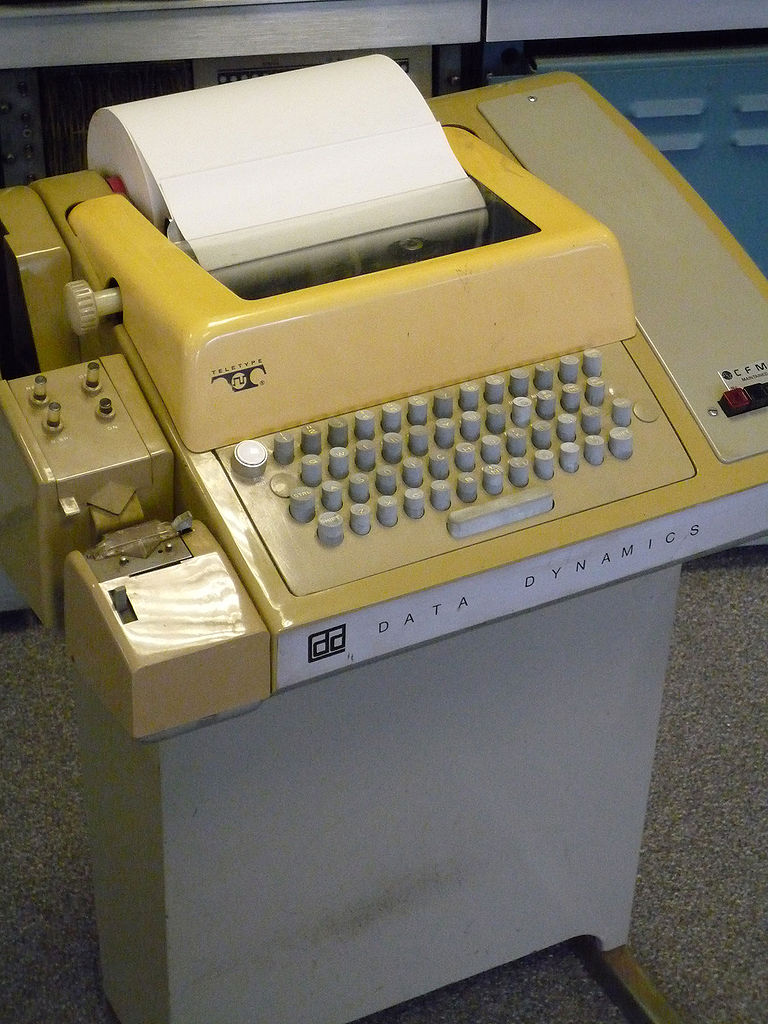
\includegraphics [width=\linewidth] {\inc/tty}
    \end {minipage}
    \hfill
    \begin {minipage} [c] {.68\linewidth}
	\begin {itemize}
	    \fB
	    \item il est relié par un lien série
		\begin {itemize}
		    \fC
		    \item paramètres : vitesse du lien, nombre
			de bits, parité
		    \item raccrocher le modem en fin de connexion
		    \item etc.
		\end {itemize}
	    \item il a des caractéristiques propres
		\begin {itemize}
		    \fC
		    \item caractères d'effacement, d'arrêt, de
			suspension, de fin de fichier, etc
		    \item bufferiser les caractères par ligne ou les
			envoyer sans attendre
		    \item nombre de lignes, de colonnes
		    \item etc.

		\end {itemize}
	\end {itemize}
    \end {minipage}

    \vspace* {2mm}

    \implique commande \code {stty} pour changer les paramètres (\implique
    \code {ioctl})

\end {frame}

\begin {frame} {Mode caractère}
    Un exemple particulier : le terminal (télétype)

    \begin {itemize}
	\fB
	\item le pilote a pour mission d'acheminer les octets
	    jusqu'au terminal

	\item certains programmes (ex: \code {zsh}, \code {vi},
	    \code {more}, etc.) doivent pouvoir en plus effacer l'écran,
	    positionner le curseur à un certain endroit, reconnaître
	    les touches de fonction, etc.

	\item séquences de contrôle différentes suivant les terminaux
	\item positionner le curseur à la ligne X et colonne Y : il faut envoyer...
	    \begin {itemize}
		\fD
		\item \framebox {ESC} \framebox {[} X \framebox {;}
		    Y \framebox {f} pour un terminal DEC VT100

		\item \framebox {ESC} \framebox {\&} \framebox {a}
		    Y \framebox {c} X \framebox {Y} pour un terminal
		    HP 2645

		\item Note : \framebox {ESC} = l'octet de code 27
	    \end {itemize}

	\item base \code {termcap}, puis \code {terminfo} pour l'ensemble
	    des séquences
	    \begin {itemize}
		\item variable d'environnement \code {TERM} : indique
		    le type de terminal
	    \end {itemize}

	\item les programmes (\code {zsh}, \code {vi}, etc.) doivent
	    utiliser cette base
	    \\
	    \implique ce n'est pas la mission du pilote

    \end {itemize}
\end {frame}

\begin {frame} {Mode caractère}
    Même principe pour la plupart des périphériques :

    \begin {itemize}
	\item le pilote achemine les octets jusqu'au périphérique
	\item ceci ne dispense pas les applications de gérer le
	    protocole de chaque périphérique

	    \begin {itemize}
		\item plusieurs protocoles différents pour les souris \\
		    \implique seul le serveur X-Window doit les connaître
		\item chaque imprimante dispose de son « langage de
		    contrôle »
		    \\
		    \implique tout programme souhaitant imprimer doit
		    disposer d'une collection d'adaptateurs pour les
		    différentes imprimantes (parfois nommés à tort
		    « pilotes »)
		\item etc.

	    \end {itemize}
    \end {itemize}
\end {frame}

\begin {frame} {Mode bloc}
    Interface du pilote :
    \begin {itemize}
	\item fonctions \code {open}, \code {close} : appelées au
	    montage/démontage du système de fichiers dans l'arborescence
	\item traitement d'interruption : idem mode brut
	\item fonction \code {strategy} : 2 rôles
	    \begin {itemize}
		\item lit un bloc en mémoire, dans le «~\textit {buffer
		    cache}~» (plus tard)
		\item écrit un bloc modifié du «~\textit {buffer cache}~»
		    vers le disque
		\item permet d'implémenter des optimisations \\
		    (ex : algorithme de l'ascenseur)
	    \end {itemize}
    \end {itemize}

    \vspace* {2mm}

    Note : la plupart des pilotes en mode bloc sont également
    accompagnés d'un pilote en mode caractère (pour \code {ioctl})
\end {frame}

\begin {frame} {Pseudo-périphériques}
    Un pilote peut offrir un service accessible via \code {read}
    ou \code {write} sans qu'il y ait un vrai périphérique

    \vspace* {3mm}

    Exemples :

    \ctableau {\fB} {|l|l|} {
	\code {/dev/null} & poubelle \\
	\code {/dev/mem} & toute la mémoire de l'ordinateur \\
	\code {/dev/random} & source d'aléa \\
    }

\end {frame}

\begin {frame} {Pseudo-périphériques}
    Cas particulier : les pseudo-terminaux

    \begin {itemize}
	\item beaucoup de programmes sont conçus pour être connectés
	    à un terminal

	\item comment fait \code {vi} lorsqu'on est connecté via
	    \code {ssh} ou via un terminal X-Window ?
	    \\
	    \implique il faut simuler un terminal et un lien série

	\item abstraction : pseudo-terminal

	    \begin {itemize}
		\item paire de pseudo-périphériques : maître et esclave
		\item gérés par le même pilote
		\item le serveur ssh gère le maître
		\item les programmes de la session accèdent
		    à l'esclave : il simule un « vrai » terminal
	    \end {itemize}
    \end {itemize}
\end {frame}

\begin {frame} {Pseudo-périphériques}

    \begin {minipage} [c] {.40\linewidth}
	\includegraphics [width=\linewidth] {\inc/pty}
    \end {minipage}
    \hfill
    \begin {minipage} [c] {.58\linewidth}
	\begin {itemize}
	    \fB
	    \item le serveur ssh ouvre la paire
	    \item tout octet émis vers le maître (resp. esclave)
		est transmis vers l'esclave (resp. maître)
	    \item le serveur ssh transmet les octets reçus depuis
		le réseau vers le maître
	    \item les programmes de la session ssh (\code {sh},
		\code {vi}) sont connectés à l'esclave
	    \item tout changement de paramètre terminal (via \code {ioctl})
		est transmis au serveur ssh
	\end {itemize}
    \end {minipage}

    \begin {itemize}
	\item autres utilisations :
	    \begin {itemize}
		\item fenêtres « terminal » en environnement graphique
		\item \code {script} (enregistrement de session)
		\item programmes \code {screen} et \code {tmux}
	    \end {itemize}
    \end {itemize}

\end {frame}

\begin {frame} {Évolutions}
    Réalité : malheureusement très complexe...
    \begin {center}
	\includegraphics [width=.6\linewidth] {\inc/arch-now}
    \end {center}

    Exemple : disques connectés via le bus SATA, SCSI,
    USB ou même via un ancestral bus IDE.

\end {frame}

\begin {frame} {Évolutions}
    \begin {itemize}
	\item complexité matérielle accrue

	    \begin {itemize}
		\item gestion des différents niveaux de bus
		\item partage de code entre pilotes (exemple : disques)
	    \end {itemize}

	\item dynamicité des périphériques

	    \begin {itemize}
		\item connecter ou déconnecter des périphériques « à chaud »
		\item auto-reconnaissance des périphériques
	    \end {itemize}
    \end {itemize}

    \implique complexité des pilotes
\end {frame}


%%%%%%%%%%%%%%%%%%%%%%%%%%%%%%%%%%%%%%%%%%%%%%%%%%%%%%%%%%%%%%%%%%%%%%%%%%%%%%
% Le répertoire /dev
%%%%%%%%%%%%%%%%%%%%%%%%%%%%%%%%%%%%%%%%%%%%%%%%%%%%%%%%%%%%%%%%%%%%%%%%%%%%%%

\titreB {Le répertoire /dev}

\begin {frame} {Le répertoire /dev}
    Historiquement, le répertoire \code {/dev} était peuplé «~à
    la main~»

    \begin {itemize}
	\item peu d'ajout ou de suppression de périphériques
	\item commande \code {mknod}
	\item script \code {MAKEDEV} dans \code {/dev}
    \end {itemize}
\end {frame}

\begin {frame} {Le répertoire /dev}
    Évolution \implique ajout dynamique de périphériques

    \begin {itemize}

	\item Système de fichier « devfs »

	    \begin {itemize}
		\item création/destruction automatique des fichiers spéciaux
		\item nécessite des périphériques capables de s'identifier
		    \begin {itemize}
			\item « plug and play »
		    \end {itemize}
	    \end {itemize}

	\item Programme additionnel pour gérer les exceptions

	    \begin {itemize}
		\item je veux un lien \code {/dev/cédérom} vers le
		    troisième lecteur de CD de mon système

		\item je veux pouvoir connecter mon appareil photo
		    sans avoir les droits de l'administrateur
	    \end {itemize}
    \end {itemize}
\end {frame}

\def\inc{inc4-ps}

\titreA {Gestion des processus}

%%%%%%%%%%%%%%%%%%%%%%%%%%%%%%%%%%%%%%%%%%%%%%%%%%%%%%%%%%%%%%%%%%%%%%%%%%%%%%
% Introduction
%%%%%%%%%%%%%%%%%%%%%%%%%%%%%%%%%%%%%%%%%%%%%%%%%%%%%%%%%%%%%%%%%%%%%%%%%%%%%%

\titreB {Introduction}

\begin {frame} {Définition d'un processus (haut niveau)}
    Définition (haut niveau) :

    \begin {quote}
	un processus est une instance d'un programme en cours d'exécution
    \end {quote}

    ... mais pas n'importe quelle exécution :

    \begin {itemize}
	\item j'exécute \code {ls /tmp} : le processus correspond à
	    l'exécution du programme \code {ls} avec les données
	    \code {/tmp}

	\item quelqu'un d'autre exécute \code {ls /tmp} en même
	    temps : ce n'est pas la même exécution, même si c'est le
	    même programme et les mêmes données

	    \begin {itemize}
		\item ce n'est pas le même processus
		\item même si le « quelqu'un d'autre », c'est moi
	    \end {itemize}

    \end {itemize}
\end {frame}

\begin {frame} {Attributs d'un processus}
    Un processus possède des attributs :

    \begin {itemize}
	\fB
	\item état (prêt à tourner, en attente, etc.)
	\item identificateur de processus (pid)
	\item identificateur de processus parent (ppid)
	\item propriétaire (uid), groupe (gid)
	\item ouvertures de fichiers
	\item répertoire courant
	\item terminal de contrôle
	\item localisation en mémoire
	\item consommation de temps CPU
	\item etc.
    \end {itemize}

\end {frame}

\begin {frame} {Définition d'un processus (bas niveau)}
    Définition (bas niveau) :

    \begin {quote}
	un processus est décrit par :
	\begin {itemize}
	    \fB
	    \item un espace mémoire pour le programme et les données
	    \item des attributs
	    \item un contexte matériel
		\begin {itemize}
		    \fC
		    \item registres du processeur
		    \item traduction d'adresses
		\end {itemize}
	\end {itemize}
    \end {quote}

    { \fB (voir \code {task\_struct} sur
	\url {http://www.tldp.org/LDP/tlk/ds/ds.html} )}

    \vspace* {2mm}

    À chaque fois :
    \begin {itemize}
	\fB
	\item qu'un processus est retiré du processeur
	    \begin {itemize}
		\fC
		\item son contexte est sauvegardé (espace mémoire, registres
		    du processeur, etc.)
	    \end {itemize}
	\item qu'un processus est mis sur le processeur
	    \begin {itemize}
		\fC
		\item son contexte est restauré
	    \end {itemize}
    \end {itemize}
\end {frame}

\begin {frame} {Espace mémoire d'un processus}
    L'espace mémoire d'un processus est découpé en 3 zones :

    \begin {minipage} [c] {.29\linewidth}
	\includegraphics [width=\linewidth] {\inc/ps-mem}
    \end {minipage}
    \hfill
    \begin {minipage} [c] {.69\linewidth}
	\begin {itemize}
	    \fB
	    \item segment « text »
		\begin {itemize}
		    \fC
		    \item programme (code compilé)
		    \item adresse 0 pas utilisée : pourquoi ?
		\end {itemize}
	    \item segment « data »
		\begin {itemize}
		    \fC
		    \item variables globales (+ \code {static} locales)
		    \item tas (mémoire allouée par \code {malloc})
		    \item extension explicite (via \code {malloc})
		\end {itemize}
	    \item segment « stack » : la pile d'exécution
		\begin {itemize}
		    \fC
		    \item variables locales
		    \item arguments des fonctions
		    \item adresses de retour
		    \item extension implicite (utilisation de la pile)
		\end {itemize}
	    \item d'autres zones peuvent être ajoutées
		\begin {itemize}
		    \fC
		    \item bibliothèques partagées
		    \item mémoire partagée entre processus
		    \item \implique cf semestre 5
		\end {itemize}
	\end {itemize}
    \end {minipage}

\end {frame}

%%%%%%%%%%%%%%%%%%%%%%%%%%%%%%%%%%%%%%%%%%%%%%%%%%%%%%%%%%%%%%%%%%%%%%%%%%%%%%
% Gestion des attributs
%%%%%%%%%%%%%%%%%%%%%%%%%%%%%%%%%%%%%%%%%%%%%%%%%%%%%%%%%%%%%%%%%%%%%%%%%%%%%%

\titreB {Gestion des attributs}

\begin {frame} {Identité}
    \prototype {
	\code {pid\_t getpid (void)} 
	\hspace* {10mm}
	\code {pid\_t getppid (void)} \\
	\code {uid\_t getuid (void)}
	\hspace* {10mm}
	\code {gid\_t getgid (void)}
    }

    \begin {itemize}
	\item Primitives simples...
	\item Ne renvoient pas -1 en cas d'erreur (pas d'erreur possible)
	\item Exemple :
	    \lstinputlisting [basicstyle=\fD\lstmonstyle] {\inc/getpid.c}
    \end {itemize}
\end {frame}

\begin {frame} {Identité}
    \prototype {
	\code {int setuid (uid\_t uid)}
	\hspace* {10mm}
	\code {int setgid (gid\_t gid)}
    }

    \begin {itemize}
	\item Primitives restreintes à l'administrateur (uid = 0)

	\item Utilisées lors de l'admission sur le système :
	    \begin {itemize}
		\item \code {/bin/login}, \code {sshd} ou équivalent pour
		    X-Window
		\item lancé par le processus numéro 1 ou un de ses
		    descendants
	    \end {itemize}
    \end {itemize}
\end {frame}

\begin {frame} {Identité}

    Algorithme de l'admission sur le système :
    \begin {enumerate}
	\item demander login et mot de passe
	\item chercher l'entrée dans \code {/etc/passwd}
	    \begin {itemize}
		\item lignes de la forme : \\
		    {\fD \code {toto:sel+mot-de-passe-chiffré:uid:gid:nom:répertoire:shell}}
		\item sel et mot de passe chiffré sont mis dans
		    un fichier séparé (\code {/etc/shadow} sur Linux)
	    \end {itemize}
	\item chiffrer le mot de passe (avec le « sel » cité
	    dans l'entrée)
	\item comparer le mot de passe avec l'entrée
	\item si identique
	    \begin {itemize}
		\item générer un nouveau processus
		\item \code {setuid (uid)} / \code {setgid (gid)}
		    dans ce nouveau processus
		\item lancer l'exécution du shell (ou du
		    «~window manager~»)
	    \end {itemize}
    \end {enumerate}
\end {frame}

\begin {frame} {Masque de création de fichiers}
    \prototype {
	\code {mode\_t umask (mode\_t masque)}
    }

    \begin {itemize}
	\item Création de fichier (\code {open (}... \code
	    {O\_CREAT}...\code {)}, \code {mkdir} ou \code {mknod})

	    \begin {itemize}
		\item permissions du fichier créé = mode \code {\& \~{}} umask
		\begin {center}
		    \includegraphics [width=.7\linewidth] {\inc/umask}
		\end {center}
	    \end {itemize}

	\item Recommandation : dans les programmes \implique 0666 ou 0777
	    \begin {itemize}
		\item les programmes sont généraux
		\item laisser l'utilisateur gérer son niveau de confidentialité
		    \begin {itemize}
			\item commande \code {umask} du Shell
		    \end {itemize}
		\item sauf pour les programmes sensibles à la sécurité
	    \end {itemize}

	\item \code {umask} renvoie l'ancien masque (avant modification)

    \end {itemize}
\end {frame}

\begin {frame} {Répertoire courant}
    \prototype {
	\code {int chdir (const char *path)}
    }

    \begin {itemize}
	\item Modifie le répertoire courant du processus
	\item Rappel : le répertoire courant est un attribut du processus
	    \begin {itemize}
		\item changer dans un processus n'affecte pas les autres
		    processus
	    \end {itemize}

	\item Pas de primitive système pour récupérer le nom
	    du répertoire courant

	    \begin {itemize}
		\item c'est une fonction de bibliothèque
		    \prototype {
			\code {char *getcwd (char *buf, size\_t max)}
		    }
		\item comment fonctionne-t'elle ?
	    \end {itemize}

    \end {itemize}
\end {frame}

\begin {frame} {Racine courante}
    \prototype {
	\code {int chroot (const char *path)}
    }

    \begin {itemize}
	\item Modifie la racine courante du processus
		\begin {center}
		    \includegraphics [width=.9\linewidth] {\inc/chroot}
		\end {center}

	\item Pas de possibilité de contournement
	    \begin {itemize}
		\item à la nouvelle racine, «~\code {..}~» reste au
		    même endroit
		\item on ne peut que descendre dans l'arborescence
	    \end {itemize}
	\item Accessible seulement à l'administrateur du système
	\item Primitive non normalisée par POSIX
    \end {itemize}
\end {frame}

\begin {frame} {Racine courante}
    \code {chroot} est un système de confinement :

    \begin {itemize}
	\item restreindre l'environnement à certains fichiers
	    seulement
	    \begin {itemize}
		\item exemple : comptes utilisateurs spécifiques
		    pour accéder à une application seulement
		\item exemple : serveur « FTP anonyme » \\
		    service FTP pour distribuer des fichiers, restreint
		    à une portion de l'arborescence

	    \end {itemize}

	\item \code {chroot} : base des systèmes de « conteneurs » modernes
		\begin {itemize}
		    \item LXC sur Linux, Jails sur FreeBSD
		    \item complété par d'autres systèmes de confinement
			\begin {itemize}
			    \item visibilité restreinte des processus
			    \item visibilité restreinte des connexions réseau
			    \item etc.
			\end {itemize}
		    \item machines « virtuelles » à moindre coût
		\end {itemize}

    \end {itemize}
\end {frame}

%%%%%%%%%%%%%%%%%%%%%%%%%%%%%%%%%%%%%%%%%%%%%%%%%%%%%%%%%%%%%%%%%%%%%%%%%%%%%%
% Création des processus
%%%%%%%%%%%%%%%%%%%%%%%%%%%%%%%%%%%%%%%%%%%%%%%%%%%%%%%%%%%%%%%%%%%%%%%%%%%%%%

\titreB {Création des processus}

\begin {frame} {Création des processus}
    \prototype {
	\code {pid\_t fork (void)}
    }

    Créer un processus $\Longleftrightarrow$ dupliquer le processus

    \begin {itemize}
	\item Primitive \code {fork} = photocopieuse à processus
	\item Processus = mémoire + attributs + contexte matériel
	    \begin {itemize}
		\item (presque) tout est dupliqué
		\item mémoire dupliquée \implique variables dupliquées
		\item les registres du CPU aussi : chaque programme
		    évoluera (registre PC) séparément
	    \end {itemize}
	\item Duplication \implique informations \textbf {héritées}
	    du processus père
	    \begin {itemize}
		\item répertoire courant, ouvertures de fichiers, etc.
		\item sauf quelques attributs~: pid, ppid, temps CPU, etc.
	    \end {itemize}
	\item Après une photocopie, on peut écrire sur chaque feuille
	    de papier, ça ne modifie pas l'autre feuille
	    \begin {itemize}
		\item c'est la même chose avec \code {fork}
	    \end {itemize}
    \end {itemize}
\end {frame}

\begin {frame} {Création des processus}
    \begin {minipage} [c] {.30\linewidth}
	\lstinputlisting [basicstyle=\fE\lstmonstyle] {\inc/fork.c}
    \end {minipage}
    \hfill
    \begin {minipage} [c] {.69\linewidth}
	\includegraphics [width=1.1\linewidth] {\inc/fork}
    \end {minipage}

    \vspace* {3mm}

    Après \code {fork} : les variables \code {x} et \code {pid}
    évoluent séparément
\end {frame}

\begin {frame} {Création des processus}
    \begin {itemize}
	\item Particularité de \code {fork} :
	    \begin {itemize}
		\item un seul appel, deux retours
		    \begin {itemize}
			\item comme \code {fork} duplique le processus,
			    tout se passe pour le deuxième comme s'il
			    avait lui-même appelé \code {fork}
		    \end {itemize}

	    \end {itemize}
	\item Valeur de retour de \code {fork} :
	    \begin {itemize}
		\item -1 en cas d'erreur (classique)
		\item 0 pour le processus fils
		\item une valeur > 0 pour le processus père
		    \begin {itemize}
			\item c'est le pid du fils
		    \end {itemize}
	    \end {itemize}
	\item Pas de déterminisme :
	    \begin {itemize}
		\item après \code {fork}, on ne sait pas si le père ou
		    le fils est remis sur le processeur en premier
		\item pas un problème : les processus évoluent indépendamment
	    \end {itemize}
    \end {itemize}
\end {frame}

\begin {frame} {Création des processus}
    \begin {itemize}
	\item Quel moyen mnémotechnique pour la valeur de retour ?
	    \begin {itemize}
		\item Chaque processus connaît son père
		    \begin {itemize}
			\item attribut ppid, primitive \code {getppid}
			\item information facile à retrouver
			\item \implique pas besoin de récupérer
			    le pid du père avec \code {fork}
			\item \code {fork} renvoie donc 0 pour le fils
		    \end {itemize}

		\item Pas de moyen facile pour récupérer le pid du fils
		    \begin {itemize}
			\item il peut y en avoir beaucoup, lequel renvoyer ?
			\item pas d'attribut, pas de primitive
			\item \implique seul moyen de récupérer le pid du
			    fils = \code {fork}
			\item \code {fork} renvoie au père le pid du fils
		    \end {itemize}
	    \end {itemize}
    \end {itemize}
\end {frame}

\begin {frame} {Création des processus}
    \begin {block} {\casseroler {Conseils pour apprivoiser \code {fork}}}

    \begin {itemize}
	\item \code {switch} avec 3 cas : \code {-1}, \code {0} et
	    \code {default}

	    \begin {itemize}
		\item pour être sûr de n'oublier aucun cas
	    \end {itemize}
	\item dans le cas 0 (fils), faire appel à une fonction \code {fils}
	    et terminer par \code {exit}
	    \begin {itemize}
		\item isoler le code du fils
		\item placer un « cordon sanitaire » afin que le fils
		    n'exécute pas le code prévu pour le père
	    \end {itemize}
    \end {itemize}
    \end {block}
\end {frame}

\begin {frame} {Création des processus}
    Exemple :

    \lstinputlisting [basicstyle=\fC\lstmonstyle] {\inc/ex-fork.c}
\end {frame}

\begin {frame} {Terminaison des processus}
    \prototype {
	\code {void exit (int code)}
    }

    \begin {itemize}
	\item Termine le processus en cours
	\item Pas de retour
	    \begin {itemize}
		\item ... et donc pas -1 en cas d'erreur
	    \end {itemize}
	\item Presque toutes les ressources sont libérées
	    \begin {itemize}
		\item mémoire, CPU, etc.
		\item cas particulier pour les processus zombies (plus tard)
	    \end {itemize}
    \end {itemize}
\end {frame}

\begin {frame} {Terminaison des processus}

    \begin {block} {\casseroler {Argument de \code {exit}}}
    \begin {itemize}
	\item code $\in$ [0..255]
	    \begin {itemize}
		\item si vous voyez \code {\alert {exit (-1)}} dans un
		    programme, c'est que son auteur n'a pas assimilé
		    son cours de système...
	    \end {itemize}
	\item valeur 0 : ok
	    \begin {itemize}
		\item convention utilisée par les shells
		\item si le père n'est pas un shell, on peut
		    utiliser une autre convention
	    \end {itemize}
	\item constantes POSIX : \code {EXIT\_SUCCESS} et \code
	    {EXIT\_FAILURE}

    \end {itemize}
    \end {block}
\end {frame}

\begin {frame} {Terminaison des processus}
    En réalité, \code {exit} est une fonction de bibliothèque
    \begin {itemize}
	\item vide les buffers des fichiers ouverts par \code {fopen}
	\item appelle les fonctions enregistrées par \code {atexit}
	\item la vraie primitive s'appelle \code {\_exit}
	    \begin {itemize}
		\item jamais appelée directement
	    \end {itemize}
    \end {itemize}
\end {frame}

\begin {frame} {Terminaison des processus}
    \prototype {
	\code {pid\_t wait (int *raison)} \\
	\code {pid\_t waitpid (pid\_t pid, int *raison, int options)} \\
    }

    \vspace* {-8mm}

    \begin {itemize}
	\item Attend la terminaison d'un des processus fils
	    \begin {itemize}
		\item \code {wait} attend n'importe quel fils
		    \begin {itemize}
			\item si un processus fils est déjà terminé,
			    pas d'attente
			\item si pas de processus fils, renvoie -1
			\item s'il y a au moins un processus fils, attente
			\item si attente interrompue par un signa, renvoie -1
		    \end {itemize}
		\item \code {waitpid} attend un processus spécifique
		    (voir manuel)
	    \end {itemize}
	\item La terminaison peut avoir plusieurs causes :
	    \begin {itemize}
		\item le fils appelle \code {exit}
		\item le fils reçoit un signal
		    \begin {itemize}
			\item \framebox {\fD CTRL} \framebox {\fD C}, violation
			    de segment, etc.
		    \end {itemize}
		\item ce peut être autre chose qu'une terminaison
		    \begin {itemize}
			\item processus ayant atteint un point d'arrêt avec
			    un débogueur
		    \end {itemize}

	    \end {itemize}
    \end {itemize}
\end {frame}

\begin {frame} {Terminaison des processus}
    \begin {itemize}
	\item Entier pointé par \code {raison} : raison de la terminaison
	    \ctableau {\fE} {|p{.2\linewidth}|p{.2\linewidth}|p{.2\linewidth}|p{.2\linewidth}|} {
		\multicolumn {1}{|c|}{\textbf {}} & 
		    \multicolumn {1}{c|}{\textbf {code retour}} &
		    \multicolumn {1}{c|}{\textbf {poids fort}} &
		    \multicolumn {1}{c|}{\textbf {poids faible}}
		    \\
		processus stoppé en mode trace &
		    identificateur~du pro\-ces\-sus &
		    numéro du signal &
		    \multicolumn {1}{c|}{0177}
		    \\
		processus terminé par exit &
		    identificateur~du pro\-ces\-sus &
		    argument de exit sur 8 bits &
		    \multicolumn {1}{c|}{0}
		    \\
		processus terminé par signal &
		    identificateur~du pro\-ces\-sus &
		    \multicolumn {1}{c|}{0} &
		    numéro du signal (+0200 si core)
		    \\
		wait interrompue par signal &
		    \multicolumn {1}{c|}{-1} &
		    \multicolumn {1}{c|}{?} &
		    \multicolumn {1}{c|}{?}
		    \\
	    }
	    \vspace* {3mm}

	\item POSIX simplifie le travail : macros les plus courantes

	    \ctableau {\fC} {|l|l|} {
		Arrêt avec \code {exit} ? & WIFEXITED () \\
		\implique si oui, code de retour & WEXITSTATUS () \\
		Arrêt sur signal ? & WIFSIGNALED () \\
		\implique si oui, numéro du signal & WTERMSIG () \\
	    }
    \end {itemize}
\end {frame}

\begin {frame} {Terminaison des processus}
    Exemple :

    \lstinputlisting [basicstyle=\fD\lstmonstyle] {\inc/ex-wait.c}
\end {frame}

\begin {frame} {Cas particulier -- Processus zombie}
    Définition :

    \begin {quote}
	Un processus zombie est un processus terminé, dont le
	père n'a pas encore enregistré la terminaison avec wait
    \end {quote}

    \begin {itemize}
	\item un processus zombie est « quasiment » terminé
	    \begin {itemize}
		\item presque toutes ses ressources sont libérées...
		\item ... sauf le descripteur du processus
		    \begin {itemize}
			\item il contient la raison de la terminaison
			\item ainsi qu'un résumé de l'utilisation
			    des ressources
		    \end {itemize}
		\item sans limitation de durée
		\item il reste visible avec \code {ps}
	    \end {itemize}


	\item lorsque le père utilise \code {wait} :

	    \begin {itemize}
		\item il collecte les informations nécessaires
		\item le descripteur de processus est libéré
		    \begin {itemize}
			\item le processus disparaît alors complètement
			    du système
		    \end {itemize}

	    \end {itemize}
    \end {itemize}
\end {frame}

\begin {frame} {Cas particulier -- Processus orphelin}
    Que se passe-t'il lorsque le père d'un processus se termine ?

    \vspace* {2mm}

    \begin {minipage} [c] {.24\linewidth}
	\includegraphics [width=\linewidth] {\inc/orphan}
    \end {minipage}
    \hfill
    \begin {minipage} [c] {.75\linewidth}
	\begin {itemize}
	    \item père se termine \implique zombie
	    \item dès que le père devient zombie, le fils est «~reparenté~»
		    (ppid $\leftarrow$ 1)
	    \item le processus 1 est spécial
		\begin {itemize}
		    \item ne s'arrête jamais
		    \item (re-)démarre les programmes du système
		    \item algorithme :
			\lstinputlisting [basicstyle=\fE\lstmonstyle] {\inc/algo-ps1.c}
		\end {itemize}
	\end {itemize}
    \end {minipage}

    \vspace* {2mm}

    \implique le fils est immédiatement reparenté \\
    \implique le statut d'orphelin n'existe donc pas dans le noyau
\end {frame}

\begin {frame} {États d'un processus}
    États d'un processus :
    \begin {center}
	\includegraphics [width=.8\linewidth] {\inc/etats}
    \end {center}
\end {frame}


%%%%%%%%%%%%%%%%%%%%%%%%%%%%%%%%%%%%%%%%%%%%%%%%%%%%%%%%%%%%%%%%%%%%%%%%%%%%%%
% Exécution d'un fichier
%%%%%%%%%%%%%%%%%%%%%%%%%%%%%%%%%%%%%%%%%%%%%%%%%%%%%%%%%%%%%%%%%%%%%%%%%%%%%%

\titreB {Exécution d'un fichier}

\begin {frame} {Exécution d'un fichier}
    \prototype {
	\fC \code {int execl (char *path, char *arg, ... )} \\
	\fC \code {int execv (char *path, char *argv [])} \\
	\fC \code {int execle (char *path, char *arg, ..., char *envp [])} \\
	\fC \code {int execve (char *path, char *argv [], char *envp [])} \\
	\fC \code {int execlp (char *fichier, char *arg0, ...)} \\
	\fC \code {int execvp (char *fichier, char *argv [])}
    }

    \begin {itemize}
	\item Primitives \code {exec*} : remplacent le programme du
	    processus courant par un nouveau programme et ses arguments

	    \begin {itemize}
		\item le contexte du processus reste quasiment inchangé
		    \begin {itemize}
			\item attributs inchangés : pid, ppid, uid
			    (sauf exception), umask, répertoire courant,
			    consommation de ressources, etc.

			\item attributs modifiés : référence à l'exécutable,
			    ouvertures de fichiers (sauf exception, notamment
			    pour 0, 1 et 2), etc.
		    \end {itemize}
		\item mémoire initialisée avec le nouveau programme
		    \begin {itemize}
			\item segments text, data et stack
		    \end {itemize}
	    \end {itemize}
	\item Valeur de retour = -1 (toujours)
	    \begin {itemize}
		\item retour \implique nouveau programme non chargé
		    \implique erreur
	    \end {itemize}
    \end {itemize}
\end {frame}

\begin {frame} {Exécution d'un fichier}
    \begin {center}
	\includegraphics [width=.8\linewidth] {\inc/exec}
    \end {center}
\end {frame}

\begin {frame} {Exécution d'un fichier -- Exemple}
    Pas de retour pour \code {exec*} \implique le plus souvent utilisée
    avec \code {fork}

    \vspace* {3mm}

    \lstinputlisting [basicstyle=\fD\lstmonstyle] {\inc/ex-exec.c}
\end {frame}

\begin {frame} {Exécution d'un fichier -- Exemple}
    Autre exemple : algorithme (grossier) du Shell

    \begin {enumerate}
	\item lire une ligne
	\item découper la ligne en éléments
	\item si éléments [0] $\in$ commandes internes
	    \begin {itemize}
		\item alors exécuter la fonction correspondante
		\item revenir en 1
	    \end {itemize}
	\item localiser le fichier éléments [0] dans \code {PATH}
	\item si pas trouvé, alors erreur et revenir en 1
	\item \code {fork} \implique fils
	    \begin {itemize}
		\item \code {exec (} éléments \code {)}
	    \end {itemize}
	\item si éléments [end] $\neq$ \code {\&}
	    \begin {itemize}
		\item alors attendre la fin du fils
	    \end {itemize}
	\item revenir en 1
    \end {enumerate}
\end {frame}

\begin {frame} {Exécution d'un fichier -- Environnement}
    En plus des arguments, \code {exec*} passe l'environnement :

    \vspace* {4mm}

    \begin {minipage} [c] {.35\linewidth}
	\includegraphics [width=1.2\linewidth] {\inc/env}
    \end {minipage}
    \hfill
    \begin {minipage} [c] {.64\linewidth}
	\begin {itemize}
	    \item \code {extern char **environ}
	    \item fonction de bibliothèque \code {getenv}
	    \item environnement modifié par le Shell
		\begin {itemize}
		    \item hérité par tous les processus lancés
			par le Shell
		    \item rappel : utiliser \code {export} en Shell pour
			exporter une variable d'environnement

		\end {itemize}
	\end {itemize}
    \end {minipage}
\end {frame}

\begin {frame} {Exécution d'un fichier}
    Six formes pour \code {exec*} :

    \begin {itemize}
	\item passage des arguments :
	    \ctableau {\fC} {|l|l|} {
		\code {execl}
		    & en liste : \code {execl (..., "echo", "a, "b", NULL)} \\
		\code {execl}
		    & en vecteur : \code {execv (..., tabargv)} \\
	    }

	    \vspace* {2mm}

	\item recherche dans la variable shell \code {PATH} :
	    \ctableau {\fC} {|l|l|} {
		\code {exec[vl]}
		    & non : \code {execv ("/bin/echo", tabargv)} \\
		\code {exec[vl]p}
		    & oui : \code {execvp ("echo", tabargv)} \\
	    }

	    \vspace* {2mm}

	\item passage de l'environnement :

	    \ctableau {\fC} {|l|l|} {
		\code {exec[vl]}
		    & implicite : \code {execv ("/bin/echo", tabargv)} \\
		\code {exec[vl]e}
		    & explicite : \code {execve ("echo", tabargv, tabenvp)} \\
	    }

    \end {itemize}

    \vspace* {2mm}

    Une seule de ces formes est une primitive système (laquelle ?) \\
    \implique les autres sont des fonctions de bibliothèque
\end {frame}

\begin {frame} {Nombres magiques}
    \code {exec*} peut exécuter plusieurs sortes de fichiers :

    \begin {itemize}
	\item Fichiers binaires (compilés)
	    \begin {itemize}
		\item plusieurs formats possibles
		    \begin {itemize}
			\item évolution des formats,
			    compatibilité avec anciennes versions
			\item sur FreeBSD : mode de compatibilité Linux
		    \end {itemize}
	    \end {itemize}
	\item Fichiers interprétés
	    \begin {itemize}
		\item fichiers non directement exécutables
		    \begin {itemize}
			\item recours à un interprète
			\item Shell, Awk, Perl, Tcl, Ruby, Python, etc.
		    \end {itemize}
		\item l'interprète ouvre le fichier et l'« exécute »
	    \end {itemize}
    \end {itemize}

    \vspace* {1mm}

    Présence d'un « nombre magique » en début de fichier

    \ctableau {\fC} {|l|l|} {
	fichiers binaires
	    & \code {0x7f 'E' 'L' 'F'} (format ELF sous Linux) \\
	fichiers interprétés
	    &  \code {'\#' '!'} (suivi du chemin de l'interprète) \\
    }

\end {frame}

%%%%%%%%%%%%%%%%%%%%%%%%%%%%%%%%%%%%%%%%%%%%%%%%%%%%%%%%%%%%%%%%%%%%%%%%%%%%%%
% Droits d'exécution
%%%%%%%%%%%%%%%%%%%%%%%%%%%%%%%%%%%%%%%%%%%%%%%%%%%%%%%%%%%%%%%%%%%%%%%%%%%%%%

\titreB {Droits d'exécution}

\begin {frame} {Droits d'exécution}
    \begin {center}
	\includegraphics [width=.8\linewidth] {\inc/droits}
    \end {center}

    \begin {itemize}
	\item \code {fork} : le fils hérite de l'uid (celui de tata)
	\item \code {exec} : ne change pas l'uid (celui de tata)
	\item le fichier \code {secret.txt} de l'utilisateur toto
	    ne peut pas être ouvert par un processus appartenant à tata
	\item \implique le système de droits fonctionne bien !

    \end {itemize}
\end {frame}

\begin {frame} {Droits d'exécution -- Élévation de privilège}
    Dans certains cas, il faut pouvoir exécuter un programme avec
    des droits plus élevés :

    \begin {itemize}
	\item un utilisateur change son mot de passe \implique
	    il doit écrire le nouveau mot de passe chiffré dans \code
	    {/etc/passwd}

	    \begin {itemize}
		\fC
		\item \code {/etc/passwd} n'est pas modifiable par
		    l'utilisateur \\
		    \fC
		    \code {\$ ls -l /etc/passwd} \\
		    \code {-rw-r--r-- 1 root 12345 Jan 1  1970 /etc/passwd}

	    \end {itemize}

	\item un utilisateur insère la carte SD de son appareil photo \\
	    \implique
	    le système de fichiers sur la carte doit être « monté »

	    \begin {itemize}
		\fC
		\item l'opération de montage (primitive système \code
		    {mount}) n'est accessible qu'à l'administrateur
	    \end {itemize}

	\item un utilisateur souhaite utiliser la commande \code {ping}

	    \begin {itemize}
		\fC
		\item \code {ping} accède aux couches réseau de bas
		    niveau et nécessite les privilèges de 
		    l'administrateur 
	    \end {itemize}

    \end {itemize}
\end {frame}

\begin {frame} {Droits d'exécution -- Élévation de privilège}
    Retour sur les permissions de fichiers :

    \begin {center}
	\includegraphics [width=.7\linewidth] {\inc/perm}
    \end {center}

    \begin {itemize}
	\item bit «~\textit {set-user-id-on-exec}~» (ou bit «~suid~»)
	\item bit «~\textit {set-group-id-on-exec}~» (ou bit «~sgid~»)
    \end {itemize}
\end {frame}

\begin {frame} {Droits d'exécution -- Bit set-user-id-on-exec}

    \begin {itemize}
	\item Appel à \code {exec} : si le bit «~suid~» est à 1,
	    alors l'uid du processus devient l'uid du propriétaire
	    du fichier

	    \begin {itemize}
		\item autrement dit : commande exécutée avec
		    les droits du propriétaire (de la commande) et non
		    ceux de l'utilisateur

	    \end {itemize}

	\item Exemple :
	    \begin {itemize}
		\item la commande \code {/bin/passwd} appartient à root
		\item dans ses permissions, le bit «~suid~» est à 1
		\item \implique le processus peut donc modifier
		    \code {/etc/passwd}
		\item \implique l'utilisateur peut changer son mot de
		    passe !
	    \end {itemize}
    \end {itemize}
\end {frame}

\begin {frame} {Droits d'exécution -- Bit set-user-id-on-exec}

    \begin {itemize}
	\item Problème 1 : \code {/bin/passwd} doit connaître l'uid de
	    l'utilisateur qui change son mot de passe...
	    \\
	    \implique 2 notions d'uid distinctes :

	    \vspace* {-2mm}

	    \ctableau {\fC} {|l|l|l|} {
		uid réel
		    & l'humain derrière son terminal
		    & \code {uid\_t getuid (void)}
		    \\
		uid effectif
		    & l'uid servant à tester les droits
		    & \code {uid\_t geteuid (void)}
		    \\
	    }
    \end {itemize}
\end {frame}

\begin {frame} {Droits d'exécution -- Bit set-user-id-on-exec}
    \begin {itemize}
	\item Problème 2 : pour certaines opérations, il faut utiliser
	    l'uid réel et non effectif
	    \begin {itemize}
		\item exemple : création de fichier
		    \implique propriétaire = uid effectif
		\item parfois, il repasser temporairement sous l'identité
		    de l'utilisateur réel
		    \begin {itemize} 
			\item exemple : pour créer le fichier sous la bonne identité
		    \end {itemize}

		\item d'où une troisième notion : uid « sauvé »
		    \begin {itemize}
			\item l'uid sauvé permet de sauver l'uid effectif
			    si jamais on le change (avec
			    \code {int seteuid (uid\_t euid)})
			\item permet de passer sous l'identité de
			    l'uid réel, puis de repasser à nouveau
			    sous l'identité privilégiée
		    \end {itemize}
	    \end {itemize}
    \end {itemize}
\end {frame}

\begin {frame} {Droits d'exécution -- Bit set-group-id-on-exec}
    Application des mêmes principes au groupe :

    \begin {itemize}
	\item bit «~set-group-id-on-exec~»
	\item 3 identités
	    \begin {itemize}
		\item gid réel
		\item gid effectif
		\item gid sauvé
	    \end {itemize}
    \end {itemize}

    \vspace* {5mm}
    Note :

    \begin {itemize}
	\item \code {ls} affiche ces bits
	\item exemple :

	    \vspace* {1mm}

	    {\fD
	    \code {\$ ls -l /usr/bin/passwd /usr/bin/crontab} \\
	    \code {-rw\alert {s}r-xr-x 1 root root\ \ \ \  12345 Jan 1  1970 /usr/bin/passwd} \\
	    \code {-rwxr-\alert {s}r-x 1 root crontab 23456 Jan 1  1970 /usr/bin/crontab}
	    }

    \end {itemize}
\end {frame}

\begin {frame} {Droits d'exécution -- Élévation de privilège}
    Bits «~suid~» et «~sgid~» : changent le niveau de privilège

    \begin {itemize}
	\item le plus souvent : pour élever le niveau
	    \begin {itemize}
		\item même si ça peut arriver de le diminuer
	    \end {itemize}

	\item ce sont des problèmes de sécurité potentiels

	    \begin {itemize}
		\item privilèges \implique attention à la programmation !
		\item bien vérifier les droits
		\item pas de « trou » de sécurité \\
		    \implique débordement de tampon, test des primitives,
		    etc.
	    \end {itemize}

	\item limiter le nombre d'exécutables avec ces bits

	    \begin {itemize}
		\item Exemple sur turing.u-strasbg.fr (Ubuntu 14.04) :

		    \ctableau {\fB} {|l|l|} {
			bit « suid » & 32 fichiers \\
			bit « sgid » & 30 fichiers \\
		    }
	    \end {itemize}
    \end {itemize}
\end {frame}


%%%%%%%%%%%%%%%%%%%%%%%%%%%%%%%%%%%%%%%%%%%%%%%%%%%%%%%%%%%%%%%%%%%%%%%%%%%%%%
% Redirections
%%%%%%%%%%%%%%%%%%%%%%%%%%%%%%%%%%%%%%%%%%%%%%%%%%%%%%%%%%%%%%%%%%%%%%%%%%%%%%

\titreB {Redirections et partage d'ouvertures de fichiers}

\begin {frame} {Redirections}
    Le Shell permet de réalise des redirections :

    \begin {itemize}
	\item \code {\$ wc -l < entree > resultat 2> erreurs}
	\item Rappel : 3 ouvertures par défaut :
	    \ctableau {\fC} {|l|l|} {
		0 & entrée standard \\
		1 & sortie standard \\
		2 & sortie d'erreur standard \\
	    }
	    \vspace* {1mm}
	\item Redirection = modification du descripteur 0, 1 ou 2
	\item À faire dans le fils (et pas dans le père), avant \code {exec}
    \end {itemize}
\end {frame}

\begin {frame} {Redirections}
    Exemple : le shell redirige la sortie standard
    \begin {enumerate}
	\item lire une ligne
	\item découper la ligne en éléments
	\item si éléments [0] $\in$ commandes internes
	    \begin {itemize}
		\item alors exécuter la fonction correspondante
		\item revenir en 1
	    \end {itemize}
	\item localiser le fichier éléments [0] dans \code {PATH}
	\item si pas trouvé, alors erreur et revenir en 1
	\item \code {fork} \implique fils
	    \begin {itemize}
		\item \code {\alert {close (1)}}
		\item \code {\alert {open ("toto", O\_WRONLY | O\_CREAT...)}}
		    \implique renvoie 1
		\item \code {exec (} éléments \code {)}
	    \end {itemize}
	\item si éléments [end] $\neq$ \code {\&}
	    \begin {itemize}
		\item alors attendre la fin du fils
	    \end {itemize}
	\item revenir en 1
    \end {enumerate}
\end {frame}

\begin {frame} {Redirections}
    Plusieurs manières de modifier les descripteurs :

    \begin {enumerate}
	\item fermer un descripteur puis ouvrir un nouveau fichier

	    \begin {itemize}
		\item cf exemple précédent
		\item par construction, \code {open} prend le plus
		    petit descripteur disponible
	    \end {itemize}
    \end {enumerate}
\end {frame}

\begin {frame} {Redirections}
    Plusieurs manières de modifier les descripteurs :

    \begin {enumerate}
	\addtocounter {enumi} {1}

	\item primitive \code {int dup (int fd)} : duplique une
	    ouverture de fichier

	    \begin {itemize}
		\item exemple :
		    \lstinputlisting [basicstyle=\fD\lstmonstyle] {\inc/ex-dup.c}
		\item intérêt : ouvrir le fichier dans le père, avant
		    \code {fork}, afin d'éviter de générer un processus
		    en cas d'erreur
	    \end {itemize}

    \end {enumerate}
\end {frame}

\begin {frame} {Redirections}
    Plusieurs manières de modifier les descripteurs :

    \begin {enumerate}
	\addtocounter {enumi} {2}
	\item primitive \code {int dup2 (int oldfd, int newfd)}

	    \begin {itemize}
		\item exemple :
		    \lstinputlisting [basicstyle=\fD\lstmonstyle] {\inc/ex-dup2.c}
		\item intérêt 1 : \code {dup2} ferme le descripteur
		    de destination si nécessaire
		\item intérêt 2 : facilite la sélection
		    du nouveau descripteur
	    \end {itemize}
    \end {enumerate}
\end {frame}

\begin {frame} {Partage d'ouvertures de fichiers -- dup/dup2}

    Structures de données du noyau :
    \begin {minipage} [c] {.65\linewidth}
	\begin {itemize}
	    \item une table globale pour toutes les ouvertures
		de fichiers
	    \item une table par processus pour ses descripteurs
	\end {itemize}
    \end {minipage}
    \hfill
    \begin {minipage} [c] {.34\linewidth}
	\lstinputlisting [basicstyle=\fE\lstmonstyle] {\inc/prtg-dup.c}
    \end {minipage}

    \begin {center}
	\includegraphics [width=.9\linewidth] {\inc/prtg-dup}
    \end {center}
\end {frame}

\begin {frame} {Partage d'ouvertures de fichiers -- dup/dup2}
    Lecture des données dans le fichier :
    \begin {minipage} [c] {.65\linewidth}
	\begin {itemize}
	    \item offset partagé entre fd1 et 5
	    \item offset propre à fd2
	\end {itemize}
    \end {minipage}
    \hfill
    \begin {minipage} [c] {.34\linewidth}
	\lstinputlisting [basicstyle=\fE\lstmonstyle] {\inc/prtg-dup.c}
    \end {minipage}

    \begin {center}
	\includegraphics [width=.8\linewidth] {\inc/prtg-data}
    \end {center}
\end {frame}

\begin {frame} {Partage d'ouvertures de fichiers -- fork}
    Que se passe-t'il si \code {fork} est appelé après une ouverture de
    fichier ?

    \begin {center}
	\includegraphics [width=.7\linewidth] {\inc/prtg-fork}
    \end {center}

    \implique partage de l'ouverture entre les deux processus
\end {frame}

\def\inc{inc5-time}

\titreA {Gestion du temps}

%%%%%%%%%%%%%%%%%%%%%%%%%%%%%%%%%%%%%%%%%%%%%%%%%%%%%%%%%%%%%%%%%%%%%%%%%%%%%%
% Introduction
%%%%%%%%%%%%%%%%%%%%%%%%%%%%%%%%%%%%%%%%%%%%%%%%%%%%%%%%%%%%%%%%%%%%%%%%%%%%%%

\titreB {Introduction}

\begin {frame} {Mesure du temps}
    Comment le noyau mesure le temps ?

    \begin {enumerate}
	\item Obtenir l'heure au démarrage
	\item Compter le temps qui passe
    \end {enumerate}
\end {frame}

\begin {frame} {Mesure du temps}
    Comment obtenir l'heure au démarrage ?
    \begin {itemize}
	\item Solution 1 : lire l'heure sur le périphérique RTC

	    \begin {itemize}
		\item RTC : \textit {Real Time Clock}
		\item horloge matérielle
		\item fonctionne sur batterie si courant coupé
	    \end {itemize}

	\item Solution 2 : demander l'heure au démarrage du noyau

	    \begin {itemize}
		\item solution « historique »
		\item encore aujourd'hui (exemple : Raspberry PI)
	    \end {itemize}

    \end {itemize}
\end {frame}

\begin {frame} {Mesure du temps}
    Comment compter le temps qui passe ?

    \begin {itemize}
	\item Le noyau doit reprendre la main à intervalle régulier
	\item Assistance matérielle indispensable
	    \begin {itemize}
		\item mécanisme d'interruption périodique du processeur
		\item historiquement : fréquence du secteur électrique
		    \begin {itemize}
			\item fréquence très stable (à l'inverse de la tension)
			\item aux États-Unis : 60 Hz \implique 60 interruptions
			    par seconde
			\item en Europe : 50 Hz \implique 50 interruptions
			    par seconde
		    \end {itemize}

		\item actuellement : composant matériel basé sur le quartz
		    \begin {itemize}
			\item fréquence programmable par le noyau
			\item en fonction de la configuration du noyau
			\item entre 50 et 1000 fois par seconde
			    (période entre 1 et 20 ms)
		    \end {itemize}
	    \end {itemize}
	\item À chaque interruption, incrémenter un compteur
	\item Lorsque le compteur atteint la fréquence
	    \begin {itemize}
		\item une seconde s'est écoulée
		\item incrémenter l'heure du système
	    \end {itemize}
    \end {itemize}
\end {frame}

\begin {frame} {Unités de temps}
    Le noyau utilise deux unités de temps :

    \begin {enumerate}
	\item instant précis dans le temps
	\item courte durée (ex : consommation de CPU)
    \end {enumerate}
\end {frame}

\begin {frame} {Unités de temps -- time\_t}

    Instant précis (à la seconde) dans le temps : type \code {time\_t}

    \begin {itemize}
	\item exemple : heure courante, date de fichier, etc.
	\item valeur : nombre de secondes depuis «~The Epoch~»
	    \begin {itemize}
		\item Epoch : premier janvier 1970, 0h0'0", UTC
		\item UTC : temps universel coordonné
		    \\
		    {\fC (avant 1986 : GMT = heure du méridien de
		    Greenwich)}

	    \end {itemize}

	\item l'heure est conservée en UTC
	    \begin {itemize}
		\item indépendamment du fuseau horaire
	    \end {itemize}

	\item \code {time\_t} historiquement sur 32 bits
	    \begin {itemize}
		\item bogue de l'an 2038 (nombre de secondes $\geq 2^{31}$)
		\item solution : passer à 64 bits (ex : Linux $\geq 3.17$)
		\item nombreux formats de fichiers avec des dates
		    sur 32 bits
	    \end {itemize}

	\item valeur de type \code {time\_t}...
	    \begin {itemize}
		\item ... facile à tenir à jour par le noyau
		\item ... pas facile à lire pour un humain
		    \begin {itemize}
			\item ce n'est pas le problème du noyau
		    \end {itemize}
	    \end {itemize}
    \end {itemize}
\end {frame}

\begin {frame} {Unités de temps -- time\_t}

    Conversion d'un \code {time\_t} en une valeur intelligible :
    \begin {itemize}
	\item problème «~intéressant~», car prise en compte :
	    \begin {itemize}
		\item du fuseau horaire
		\item de l'heure d'été et de l'heure d'hiver
		\item des changements de dates des heures d'été et d'hiver
		    \begin {itemize}
			\item ex : pas de changement d'heure avant 1976
			    en France
		    \end {itemize}
		\item des années bissextiles
		\item des secondes intercalaires
		    \begin {itemize}
			\item variations de la vitesse de rotation de la Terre
			\item ex : 1 seconde ajoutée après 23h59'59"
			    le 31/12/2016
		    \end {itemize}
	    \end {itemize}

	\item ... mais ne concerne pas le noyau
	\item \implique à la charge des fonctions de bibliothèque
	    \begin {itemize}
		\item \code {localtime}, \code {asctime}, \code {strftime}, etc.
	    \end {itemize}

    \end {itemize}
\end {frame}

\begin {frame} {Unités de temps -- clock\_t}
    courte durée : type \code {clock\_t}

    \begin {itemize}
	\item exemple : temps CPU consommé par un processus
	\item valeur : nombre de tops d'horloge (ou «~\textit {ticks}~»)
	\item unité dépend de la configuration du noyau
	    \begin {itemize}
		\item POSIX fournit la primitive
		    \code {long sysconf (int paramètre})
		\item \code {paramètre} : paramètre de configuration interrogé
		\item exemple : \code {freq = sysconf (\_SC\_CLK\_TCK)}
		    \\
		    \implique donne le nombre de tops d'horloge par seconde
	    \end {itemize}
	\item mesure de la consommation CPU :
	    \begin {itemize}
		\item à chaque interruption d'horloge, le noyau incrémente
		    le compteur du processus courant
		\item \implique consommation approximative
	    \end {itemize}
    \end {itemize}
\end {frame}

%%%%%%%%%%%%%%%%%%%%%%%%%%%%%%%%%%%%%%%%%%%%%%%%%%%%%%%%%%%%%%%%%%%%%%%%%%%%%%
% Heure courante
%%%%%%%%%%%%%%%%%%%%%%%%%%%%%%%%%%%%%%%%%%%%%%%%%%%%%%%%%%%%%%%%%%%%%%%%%%%%%%

\titreB {Heure courante}

\begin {frame} {Heure courante}
    \prototype {
	\code {time\_t time (time\_t *heure)} \\
	\code {int stime (time\_t *heure)}
    }

    \begin {itemize}
	\item \code {time} récupère l'heure courante
	    \begin {itemize}
		\item comme valeur de retour (ou -1)
		\item et à l'adresse indiquée
	    \end {itemize}
	\item \code {stime} modifie l'heure courante
	    \begin {itemize}
		\item primitive réservée à l'administrateur
	    \end {itemize}
    \end {itemize}

    \vspace* {3mm}

    Note : l'heure courante est parfois appelée «~\textit {wall clock}~» \\
    (i.e. l'heure qu'on peut lire sur l'horloge murale)
\end {frame}

\begin {frame} {Heure courante -- gettimeofday}
    \prototype {
	\code {int gettimeofday (struct timeval *tv, struct timezone *tz)}
    }

    \begin {itemize}
	\item ajout de l'U. de Berkeley
	\item précision accrue
	\item contenu de la \code {struct timeval} :
	    \ctableau {\fD} {|ll|l|} {
		\code {time\_t} & \code {tv\_sec}
		    & nombre de secondes depuis « The Epoch » \\
		\code {suseconds\_t}  & \code {tv\_usec}
		    & nombre de micro-secondes \\
	    }

	    \vspace* {1mm}

	\item attention : ce n'est pas parce qu'il y a un champ dont
	    l'unité est la $\mu$s que la granularité de la mesure
	    du temps est la $\mu$s

	\item \code {time} est maintenant devenue une fonction de
	    bibliothèque qui appelle la primitive \code {gettimeofday}

    \end {itemize}
\end {frame}

\begin {frame} {Heure courante -- gettimeofday}
    Exemple de \code {struct timeval}~:

    \vspace* {3mm}
    
    \begin {minipage} {.35\linewidth}
    \ctableau {\fD} {|l|r|} {
	\code {tv\_sec}
	    & 1$\thinspace$500$\thinspace$000$\thinspace$000
	    \\
	\code {tv\_usec}
	    & 123$\thinspace$456
	    \\
    }
    \end {minipage}
    \hfill
    $\Leftrightarrow$
    \hfill
    \begin {minipage} {.55\linewidth}
	\fC 14/07/2017 à 2h40'00" et 123456 $\mu s$ UTC
    \end {minipage}


    \begin {center}
	\includegraphics [width=.9\linewidth] {\inc/timeval}
    \end {center}
\end {frame}


\begin {frame} {Heure courante}
    Exemple d'utilisation :

    \lstinputlisting [basicstyle=\fD\lstmonstyle] {\inc/ex-lib.c}

    \begin {itemize}
	\item « primitive système » : \code {time}
	\item fonctions de bibliothèque : \code {localtime}, \code
	    {asctime} et \code {strftime}
    \end {itemize}
\end {frame}

%%%%%%%%%%%%%%%%%%%%%%%%%%%%%%%%%%%%%%%%%%%%%%%%%%%%%%%%%%%%%%%%%%%%%%%%%%%%%%
% Temps CPU
%%%%%%%%%%%%%%%%%%%%%%%%%%%%%%%%%%%%%%%%%%%%%%%%%%%%%%%%%%%%%%%%%%%%%%%%%%%%%%

\titreB {Temps CPU}

\begin {frame} {Temps CPU}
    \prototype {
	\code {clock\_t times (struct tms *buf)} \\
    }

    \begin {itemize}
	\item place la consommation CPU à l'adresse pointée par \code {buf}
	    \begin {itemize}
		\item contenu de la \code {struct tms}~:

		    \vspace* {-3mm}

		    \ctableau {\fD} {|l|l|} {
			\code {tms\_utime}
			    & consommation CPU du processus
				en mode utilisateur \\
			\code {tms\_stime}
			    & consommation CPU du processus
				en mode système \\
			\code {tms\_cutime}
			    & consommation CPU cumulée des fils
				en mode utilisateur \\
			\code {tms\_cstime}
			    & consommation CPU cumulée des fils
				en mode système \\
		    }

		    \vspace* {1mm}

		\item tous les champs sont de type \code {clock\_t}
	    \end {itemize}

	\item retourne le temps réellement écoulé depuis un moment
	    arbitraire dans le passé (ou -1)

	    \begin {itemize}
		\item typiquement le démarrage du noyau
		\item pas très utile
		\item peut déborder la taille allouée à un \code {clock\_t}
		\item bref : valeur de retour à ignorer (sauf pour test
		    d'erreur)...
	    \end {itemize}

    \end {itemize}
\end {frame}

\begin {frame} {Temps CPU}
    Récupération de la consommation CPU :

    \begin {center}
	\includegraphics [width=.5\linewidth] {\inc/times}
    \end {center}

    \begin {itemize}
	\item état « zombie » : permet de transmettre 3 informations
	    \begin {itemize}
		\item code de retour (primitive \code {exit})
		\item consommation CPU agrégée en mode utilisateur
		\item consommation CPU agrégée en mode système
	    \end {itemize}
	\item informations transmises lors du \code {wait} par le père
	\item on ne peut pas avoir la consommation d'un fils non terminé
    \end {itemize}

\end {frame}

\begin {frame} {Temps CPU}
    \prototype {
	\code {int getrusage (int qui, struct rusage *res)}
    }

    \begin {itemize}
	\item primitive \code {times} limitée à la consommation CPU
	\item \implique besoin d'une primitive plus générale pour
	    l'ensemble des ressources consommées par un processus
	\item paramètre \code {qui} :
	    \ctableau {\fD} {|l|l|} {
		\code {RUSAGE\_SELF}
		    & consommation du processus lui-même \\
		\code {RUSAGE\_CHILDREN}
		    & consommation cumulée des fils \\
	    }
	    \vspace* {1mm}
	\item exemples (non exhaustifs) de champs de \code {struct rusage} :

	    \ctableau {\fD} {|l|l|} {
		\code {ru\_utime} & CPU en mode utilisateur \\
		\code {ru\_stime} & CPU en mode système \\
		\code {ru\_maxrss} & mémoire maximum utilisée \\
		\code {ru\_inblock} & nombre de lectures disques \\
		\code {ru\_outblock} & nombre d'écritures disques \\
	    }
    \end {itemize}
\end {frame}

%%%%%%%%%%%%%%%%%%%%%%%%%%%%%%%%%%%%%%%%%%%%%%%%%%%%%%%%%%%%%%%%%%%%%%%%%%%%%%
% Dates des fichiers
%%%%%%%%%%%%%%%%%%%%%%%%%%%%%%%%%%%%%%%%%%%%%%%%%%%%%%%%%%%%%%%%%%%%%%%%%%%%%%

\titreB {Dates des fichiers}

\begin {frame} {Dates des fichiers}
    \vspace* {-2mm}
    \prototype {
	\code {int utime (const char *path, const struct utimbuf *ut)}
	\\
	\code {int utimes (const char *path, const struct timeval tv [2])}
    }

    \vspace* {-2mm}

    \begin {itemize}
	\item Rappel des attributs des fichiers :

	    \ctableau {\fD} {|l|l|} {
		\code {st\_mtime}
		    & date de dernière modification des données \\
		\code {st\_ctime}
		    & date de dernière modification de l'inode \\
		\code {st\_atime}
		    & date de dernier accès \\
	    }

	    \vspace* {1mm}

	\item Primitive \code {utime} : modification des dates d'un
	    fichier
	\item Champs de la \code {struct utimbuf} :
	    \ctableau {\fD} {|l|l|} {
		\code {actime} & date de dernier accès \\
		\code {modtime} & date de dernière modification des
		    données \\
	    }

	    \vspace* {1mm}

	\item Pas de dernière modification de l'inode \implique pourquoi ?

	\item Primitive \code {utimes} : idem \code {utime}, mais avec
	    des \code {struct timeval} (comme \code {gettimeofday})
	    \begin {itemize}
		\item \code {tv[0]} : dernier accès
		\item \code {tv[1]} : dernière modification des données
	    \end {itemize}
    \end {itemize}
\end {frame}

%%%%%%%%%%%%%%%%%%%%%%%%%%%%%%%%%%%%%%%%%%%%%%%%%%%%%%%%%%%%%%%%%%%%%%%%%%%%%%
% Alarmes de processus
%%%%%%%%%%%%%%%%%%%%%%%%%%%%%%%%%%%%%%%%%%%%%%%%%%%%%%%%%%%%%%%%%%%%%%%%%%%%%%

\titreB {Alarmes de processus}

\begin {frame} {Alarmes de processus}
    Voir chapitre suivant (signaux)
\end {frame}

%%%%%%%%%%%%%%%%%%%%%%%%%%%%%%%%%%%%%%%%%%%%%%%%%%%%%%%%%%%%%%%%%%%%%%%%%%%%%%
% Précision de la mesure du temps
%%%%%%%%%%%%%%%%%%%%%%%%%%%%%%%%%%%%%%%%%%%%%%%%%%%%%%%%%%%%%%%%%%%%%%%%%%%%%%

\titreB {Précision de la mesure du temps}

\begin {frame} {Précision de la mesure du temps}
    La précision de la mesure de la consommation de temps CPU est
    approximative

    \begin {center}
	\includegraphics [width=.9\linewidth] {\inc/precision}
    \end {center}

    \begin {itemize}
	\item comptabilisation du temps pour un processus lorsque
	    l'horloge interrompt le CPU
	    \begin {itemize}
		\item pas de prise en compte du temps de B avant son E/S
		    \\
		    \implique temps imputé à C
		\item l'interruption disque est traitée alors que le
		    A est sur le CPU \\
		    \implique temps pour traitement d'E/S de B
			imputé à A
	    \end {itemize}

	\item \implique faire plusieurs mesures
    \end {itemize}

\end {frame}

\def\inc{inc6-pipe}

\titreA {Gestion des tubes}

%%%%%%%%%%%%%%%%%%%%%%%%%%%%%%%%%%%%%%%%%%%%%%%%%%%%%%%%%%%%%%%%%%%%%%%%%%%%%%
% Introduction
%%%%%%%%%%%%%%%%%%%%%%%%%%%%%%%%%%%%%%%%%%%%%%%%%%%%%%%%%%%%%%%%%%%%%%%%%%%%%%

\titreB {Introduction}

\begin {frame} {Introduction}
    Les tubes sont une des innovations majeures d'Unix

    \begin {itemize}
	\item exemple en Shell : \code {\$ ls -l | wc -l}

	    \begin {center}
		\includegraphics [width=.8\linewidth] {\inc/principe}
	    \end {center}

	\item le processus \code {ls} écrit dans le tube
	    \begin {itemize}
		\item utilisation de la primitive \code {write}
		\item si \code {ls} écrit trop vite (\implique tube plein),
			\code {write} attend
	    \end {itemize}
	\item le processus \code {wc} lit dans le tube
	    \begin {itemize}
		\item utilisation de la primitive \code {read}
		\item si \code {wc} lit trop vite (\implique tube vide),
		    \code {read} attend
	    \end {itemize}
	\item les deux processus tournent en parallèle
	    \begin {itemize}
		\item synchronisation implicite
	    \end {itemize}
	\item pas de limitation sur la quantité de données transférée
    \end {itemize}
\end {frame}

%%%%%%%%%%%%%%%%%%%%%%%%%%%%%%%%%%%%%%%%%%%%%%%%%%%%%%%%%%%%%%%%%%%%%%%%%%%%%%
% Création des tubes
%%%%%%%%%%%%%%%%%%%%%%%%%%%%%%%%%%%%%%%%%%%%%%%%%%%%%%%%%%%%%%%%%%%%%%%%%%%%%%

\titreB {Création des tubes}

\begin {frame} {Création des tubes}
    \prototype {
	\code {int pipe (int tube [2])}
    }

    \begin {itemize}
	\item création du tube et de deux descripteurs
	\item après appel à \code {pipe} :
	    \begin {center}
		\includegraphics [width=.7\linewidth] {\inc/creation-0}
	    \end {center}
	\item lecture via \code {tube [0]}
	\item écriture via \code {tube [1]}
	\item utilité : avec \code {fork}...
    \end {itemize}
\end {frame}


\begin {frame} {Exemple [1/6]}
    \begin {center}
	\includegraphics [width=\linewidth] {\inc/creation-1}
    \end {center}
\end {frame}

\begin {frame} {Exemple [2/6]}
    \begin {center}
	\includegraphics [width=\linewidth] {\inc/creation-2}
    \end {center}
\end {frame}

\begin {frame} {Exemple [3/6]}
    \begin {center}
	\includegraphics [width=\linewidth] {\inc/creation-3}
    \end {center}
\end {frame}

\begin {frame} {Exemple [4/6]}
    \begin {center}
	\includegraphics [width=\linewidth] {\inc/creation-4}
    \end {center}
\end {frame}

\begin {frame} {Exemple [5/6]}
    \begin {center}
	\includegraphics [width=\linewidth] {\inc/creation-5}
    \end {center}
\end {frame}

\begin {frame} {Exemple [6/6]}
    \begin {center}
	\includegraphics [width=\linewidth] {\inc/creation-6}
    \end {center}
\end {frame}

%%%%%%%%%%%%%%%%%%%%%%%%%%%%%%%%%%%%%%%%%%%%%%%%%%%%%%%%%%%%%%%%%%%%%%%%%%%%%%
% Règles de fonctionnement
%%%%%%%%%%%%%%%%%%%%%%%%%%%%%%%%%%%%%%%%%%%%%%%%%%%%%%%%%%%%%%%%%%%%%%%%%%%%%%

\titreB {Règles de fonctionnement}

\begin {frame} {Règles de fonctionnement [1/3]}
    Règles particulières des tubes pour la lecture (\code {read}) :

    \begin {itemize}
	\item Primitive \code {read} bloquante
	    \begin {itemize}
		\item \code {read} renvoie 0 quand tube vide et plus
		    aucun écrivain
	    \end {itemize}

	\item Lectures partielles
	    \begin {itemize}
		\item \code {read} renvoie ce qui est disponible dans le tube
		\item vraisemblablement moins que ce qui est demandé
		\item \implique être prêt à ce que \code
		    {read} renvoie moins que demandé
	    \end {itemize}
    \end {itemize}
\end {frame}

\begin {frame} {Règles de fonctionnement [2/3]}
    Règles particulières des tubes pour l'écriture (\code {write}) :

    \begin {itemize}
	\item Écritures partielles
	    \begin {itemize}
		\item \code {write} limité par taille maximum des tubes
		\item taille maximum variable (même sur le même système)
		\item \implique être prêt à ce que \code{write}
		    renvoie moins que demandé

	    \end {itemize}

	\item Écriture dans un tube sans lecteur
	    \implique problème !
	    \begin {itemize}
		\item renvoyer \code {-1} ne suffit pas
		    \begin {itemize}
			\item programmes mal écrits ne testent pas
			    les erreurs...
		    \end {itemize}
		\item envoi du signal \code {SIGPIPE} \implique
		    terminaison du processus
		\item exemple : \code {\$ find / | ./a.out}
		    \begin {itemize}
			\item arrêt « prématuré » de \code {a.out} \implique
			    arrêt automatique de \code {find}
			    sans continuer à générer des données inutiles
		    \end {itemize}
	    \end {itemize}
    \end {itemize}
\end {frame}

\begin {frame} {Règles de fonctionnement [3/3]}
    Règles particulières pour le partage des tubes :

    \begin {itemize}
	\item Il peut y avoir plusieurs lecteurs et plusieurs écrivains
	    \begin {itemize}
		\item situation « normale » (exemple : juste après \code {fork})
		\item attention à la détection de « fin de fichier »
		    \begin {itemize}
			\item plus aucun écrivain...
			\item \implique fermer les descripteurs dès
			    qu'ils ne sont plus utilisés
		    \end {itemize}
	    \end {itemize}

	\item Écritures simultanées par plusieurs écrivains
	    \begin {itemize}
		\item taille $\leq$ \code {PIPE\_BUF} : pas de mélange
		    entre écrivains
		\item taille $>$ \code {PIPE\_BUF} : mélange possible
		    entre écrivains
		\item \code {PIPE\_BUF} = 512 (FreeBSD) ou 4096 (Linux)
	    \end {itemize}

    \end {itemize}
\end {frame}

\begin {frame} {Ne pas oublier...}
    \begin {block} {\casseroler {Principes à respecter}}

    \begin {itemize}
	\item l'appel à \code {pipe} doit être fait \alert {avant}
	    l'appel à \code {fork}
	    \begin {itemize}
		\item sinon le tube n'est pas hérité
	    \end {itemize}
	\item \alert {fermer} les descripteurs dès qu'ils ne sont
	    plus utilisés
	    \begin {itemize}
		\item indispensable dans certains cas avec les tubes
		\item \implique le faire systématiquement évite d'avoir
		    à réfléchir !
	    \end {itemize}
    \end {itemize}
    \end {block}
\end {frame}

%%%%%%%%%%%%%%%%%%%%%%%%%%%%%%%%%%%%%%%%%%%%%%%%%%%%%%%%%%%%%%%%%%%%%%%%%%%%%%
% Tubes nommés
%%%%%%%%%%%%%%%%%%%%%%%%%%%%%%%%%%%%%%%%%%%%%%%%%%%%%%%%%%%%%%%%%%%%%%%%%%%%%%

\titreB {Tubes nommés}

\begin {frame} {Tubes nommés}
    \prototype {\code {int mkfifo (const char *path, mode\_t mode)}}

    \begin {itemize}
	\item Tubes créés par \code {pipe} : tubes anonymes
	    \begin {itemize}
		\item doivent être créés par un ancêtre commun aux
		    processus
		\item héritage des descripteurs d'ouverture
	    \end {itemize}
	\item Tubes nommés : nom de fichier dans l'arborescence
	\item Nouveau type de fichier : «~\textit {fifo}~»
	    \begin {itemize}
		\item avec \code {stat} : \code {S\_IFIFO} et
		    \code {S\_ISFIFO()}
	    \end {itemize}
	\item Création avec \code {mkfifo}
	    \begin {itemize}
		\item accès ultérieur avec \code {open}, \code {read},
		    \code {write}, et \code {close}
		\item \implique comme avec n'importe quel fichier régulier
	    \end {itemize}
	\item Règles de fonctionnement : cf tubes anonymes
	    \begin {itemize}
		\item ... après démarrage d'un lecteur et d'un écrivain
		\item \code {read} ou \code {write} bloqué en attendant
		    l'autre partie
	    \end {itemize}
    \end {itemize}
\end {frame}

%%%%%%%%%%%%%%%%%%%%%%%%%%%%%%%%%%%%%%%%%%%%%%%%%%%%%%%%%%%%%%%%%%%%%%%%%%%%%%
% Redirections
%%%%%%%%%%%%%%%%%%%%%%%%%%%%%%%%%%%%%%%%%%%%%%%%%%%%%%%%%%%%%%%%%%%%%%%%%%%%%%

\titreB {Redirections}

\begin {frame} {Redirections}

    \begin {itemize}
	\item Comment faire la redirection avec un tube ?
	    \begin {itemize}
		\item exemple : \code {\$ ls -l | wc -l}
	    \end {itemize}

	\item Principe similaire aux redirections classiques
	    \begin {enumerate}
		\item créer un tube anonyme avant le \code {fork}
		\item dans le processus écrivain (ici \code {ls}) :
		    \begin {enumerate}
			\item \code {dup2 (tube [1], 1)}
			\item \code {close (tube [0])}
			\item \code {close (tube [1])}
		    \end {enumerate}
		\item dans le processus lecteur (ici \code {wc}) :
		    \begin {enumerate}
			\item \code {dup2 (tube [0], 0)}
			\item \code {close (tube [0])}
			\item \code {close (tube [1])}
		    \end {enumerate}
	    \end {enumerate}
    \end {itemize}
\end {frame}

\def\inc{inc7-sig}

\titreA {Gestion des signaux}

%%%%%%%%%%%%%%%%%%%%%%%%%%%%%%%%%%%%%%%%%%%%%%%%%%%%%%%%%%%%%%%%%%%%%%%%%%%%%%
% Introduction
%%%%%%%%%%%%%%%%%%%%%%%%%%%%%%%%%%%%%%%%%%%%%%%%%%%%%%%%%%%%%%%%%%%%%%%%%%%%%%

\titreB {Introduction}

\begin {frame} {Introduction}
    Définition
    \begin {quote}
	Un signal est un événement notifié par le noyau à un processus
    \end {quote}

    \vspace* {-2mm}
    
    Exemples :
    \begin {itemize}
	\item événements matériels
	    \begin {itemize}
		\item déconnexion (\code {SIGHUP}),
		\item appui sur \framebox {\fC CTRL}\framebox {\fC C}
		    (\code {SIGINT})
	    \end {itemize}
	\item événements suite à une action du programme
	    \begin {itemize}
		\item erreur d'adressage mémoire (\code {SIGSEGV})
		\item instruction illégale (\code {SIGILL}),
		\item alarme de processus (\code {SIGALRM}),
		\item écriture dans un tube sans lecteur (\code {SIGPIPE}), etc
	    \end {itemize}
	\item événements sans sémantique associée pour le noyau
	    \begin {itemize}
		\item signaux « utilisateur » (\code {SIGUSR1} et
		    \code {SIGUSR2})
		\item signal de terminaison (\code {SIGTERM})
		\item signal de terminaison absolu (\code {SIGKILL})
	    \end {itemize}

    \end {itemize}

    Les signaux sont représentés par des entiers \implique \code {SIG*}
\end {frame}

\begin {frame} {Introduction}
    Notification au processus \implique actions possibles du processus :

    \begin {itemize}
	\item ignorer le signal
	    \begin {itemize}
		\item action par défaut pour quelques rares signaux
		\item exemple : \code {SIGCHLD} \implique terminaison
		    d'un fils
	    \end {itemize}
	\item terminer le processus
	    \begin {itemize}
		\item action par défaut pour la plupart des signaux
		\item exemple : \code {SIGSEGV} \implique erreur
		    d'adressage mémoire
		\item certains signaux provoquent la génération d'un
		    fichier \code {core}
		    \begin {itemize}
			\item pour l'analyse de la mémoire à postériori
			\item exemple : \code {\$ gdb a.out core}
			\item peut nécessiter : \code {\$ ulimit
			    -c unlimited}

		    \end {itemize}
	    \end {itemize}
	\item exécuter une fonction spécifiée préalablement
	    \begin {itemize}
		\item la fonction interrompt l'exécution du programme
		\item lorsque la fonction se termine, le programme reprend
		    où il avait été interrompu
	    \end {itemize}
    \end {itemize}
\end {frame}

\begin {frame} {Exemples d'utilisation des signaux}

    \begin {itemize}
	\item sauvegarder le calcul en cours en cas d'interruption
	    \begin {itemize}
		\item appui sur \framebox {\fC CTRL}\framebox {\fC C}
		    \implique \code {SIGINT}
		\item appeler la fonction programmée pour \code {SIGINT}
	    \end {itemize}

	\item interrompre une action sans sortir du programme
	    \begin {itemize}
		\item exemple : \framebox {\fC CTRL}\framebox {\fC C}
		    avec \code {vi}
	    \end {itemize}

	\item terminer le programme proprement
	    \begin {itemize}
		\item l'utilisateur envoie le signal \code {SIGTERM}
		\item appeler la fonction programmée pour \code {SIGTERM}
		    \begin {itemize}
			\item sauvegarder les données en mémoire,
			    supprimer les fichiers temporaires, etc.
		    \end {itemize}
	    \end {itemize}

	\item continuer le programme même après une déconnexion
	    \begin {itemize}
		\item déconnexion \implique \code {SIGHUP}
		\item ignorer le signal
	    \end {itemize}

	\item planifier une action à exécuter dans 3 minutes
	    \begin {itemize}
		\item programmer une alarme \implique \code {SIGALRM}
		\item appeler la fonction programmée pour \code {SIGALRM}
	    \end {itemize}
    \end {itemize}
\end {frame}

\begin {frame} {Cas particulier -- SIGKILL}
    \begin {itemize}
	\item Avec les signaux, il est possible d'exécuter une fonction
	    au lieu de terminer le processus par défaut

	\item S'il est possible de programmer une fonction pour chacun
	    des signaux, on peut avoir des processus «~immortels~»

	\item D'où le signal \code {SIGKILL} :

	    \begin {itemize}
		\item action = action par défaut
		    \implique terminer le processus
		\item impossible de changer cette action
		\item il reste toujours un moyen de terminer un processus !
	    \end {itemize}

    \end {itemize}
\end {frame}

%%%%%%%%%%%%%%%%%%%%%%%%%%%%%%%%%%%%%%%%%%%%%%%%%%%%%%%%%%%%%%%%%%%%%%%%%%%%%%
% API Unix v7
%%%%%%%%%%%%%%%%%%%%%%%%%%%%%%%%%%%%%%%%%%%%%%%%%%%%%%%%%%%%%%%%%%%%%%%%%%%%%%

\titreB {API Unix v7}

\begin {frame} {API Unix v7}
    Ensemble de primitives pour gérer les signaux :

    \vspace* {-3mm}

    \prototype {
	\code {void (*signal (int sig, void (*fct) (int sig))) (int sig)} \\
	\code {int kill (pid\_t pid, int sig)} \\
	\code {int pause (void)} \\
	\code {unsigned int alarm (unsigned int nsec)}
    }

    \vspace* {-2mm}

    \begin {itemize}
	\item primitives « originelles » (Unix v7, 1977)
	    \begin {itemize}
		\item en réalité plus anciennes
		\item mais Unix v7 très largement diffusé

	    \end {itemize}
	\item primitive \code {signal} obsolète
	    \begin {itemize}
		\item supplantée par \code {sigaction}, voir API POSIX
		\item mais \code {signal} simple, toujours utilisée
		\item et bonne introduction pédagogique
		\item et malgré tout, toujours normalisée par POSIX
	    \end {itemize}
	\item les autres primitives sont toujours d'actualité
    \end {itemize}
\end {frame}

\begin {frame} {API Unix v7 -- Primitive signal}
    \begin {minipage} [c] {.50\linewidth}
	\hspace* {-5mm}
	\includegraphics [width=1.1\linewidth] {\inc/derout}
    \end {minipage}
    \hfill
    \begin {minipage} [c] {.49\linewidth}
	\fC
	\begin {itemize}
	    \item \code {signal} définit l'action à réaliser
		lorsque le signal \textbf {arrivera}
	    \item prototype \code {fct} fixe
		\begin {itemize}
		    \fD
		    \item numéro de signal passé en
			argument
		    \item pas d'autre argument possible
		\end {itemize}
	\end {itemize}
    \end {minipage}

    \vspace* {5mm}

    Autres valeurs possibles pour la fonction de \code {signal} :

    \vspace* {-3mm}

    \ctableau {\fC} {|l|p{.8\linewidth}|} {
	\code {SIG\_IGN} & ignorer le signal \\
	\code {SIG\_DFL} & remettre l'action par défaut (plupart
	    des signaux : terminer le processus) \\
    }
\end {frame}

\begin {frame} {API Unix v7 -- Primitive signal}
    \prototype {
	\code {void (*signal (int sig, void (*fct) (int sig))) (int sig)}
    }

    \begin {itemize}
	\item quel beau prototype de fonction C...
	\item \code {signal} prend en argument : :
	    \begin {itemize}
		\item un numéro de signal pour lequel
		    l'action doit être définie
		\item l'adresse d'une fonction (dans le programme)
		    \begin {itemize}
			\item prenant en argument un entier
			    (le numéro du signal reçu)
			\item et ne renvoyant rien
		    \end {itemize}
		    ou bien :
		    \begin {itemize}
			\item \code {SIG\_DFL} : adresse == 0 
			\item \code {SIG\_IGN} : adresse == 1
		    \end {itemize}
	    \end {itemize}
	\item \code {signal} renvoie l'adresse de l'ancienne fonction
	    \begin {itemize}
		\item ou bien \code {SIG\_ERR} (adresse == -1) en cas d'erreur
		    \begin {itemize}
			\item par exemple si \code {sig} == \code {SIGKILL}
		    \end {itemize}
	    \end {itemize}
	\item attention : \code {signal (SIGHUP, fct (5))} passe en
	    argument le \textbf {résultat} de l'appel de la fonction
	    \code {fct}, et non son adresse

    \end {itemize}
\end {frame}

\begin {frame} {API Unix v7 -- Fonction appelée}
    La fonction appelée doit avoir le prototype suivant :

    \lstinputlisting [basicstyle=\fD\lstmonstyle] {\inc/proto.c}

    Notes :
    \begin {itemize}
	\item pas de possibilité de changer le type de retour
	\item pas de possibilité de changer les arguments

	\item avec les options \code {-Wall -Werror} du
	    compilateur \code {gcc}, il faut éviter de générer une
	    erreur si l'argument n'est pas utilisé

	    \lstinputlisting [basicstyle=\fD\lstmonstyle] {\inc/unused.c}
    \end {itemize}

\end {frame}

\begin {frame} {API Unix v7 -- Fonction appelée}
    Attention à la fonction appelée lors de la réception d'un signal :

    \begin {itemize}
	\item L'appel de la fonction interrompt le programme en
	    cours
	\item Le programme pouvait faire des choses complexes

	    \begin {itemize}
		\item exemple~:

		    \lstinputlisting [basicstyle=\fE\lstmonstyle, numbers=left] {\inc/compteur.c}
	    \end {itemize}

	\item Problème :
	    \begin {itemize}
		\item si le programme est interrompu entre les lignes 11 et 12
		\item et si la fonction utilise la variable \code {c}
	    \end {itemize}
    \end {itemize}
\end {frame}

\begin {frame} {API Unix v7 -- Fonction appelée}
    Recommandations pour la fonction :

    \begin {itemize}
	\item Limiter la fonction à la modification d'une variable
	\item Tester la variable dans le programme principal
	\item Utiliser une variable « \code {volatile sig\_atomic\_t} »
	    \begin {itemize}
		\item qualificateur \code {volatile} : empêcher
		    certaines optimisations intempestives
		\item type \code {sig\_atomic\_t} : variable modifiée
		    en une seule opération
		    \\
		    \implique voir cours de Systèmes Concurrents en L3S5
	    \end {itemize}
    \end {itemize}

    \vspace* {3mm}

    Autre action dans la fonction \implique fonctionnement
    non garanti
\end {frame}

\begin {frame} {API Unix v7 -- Fonction appelée}
    Exemple :

    \lstinputlisting [basicstyle=\fD\lstmonstyle, firstline=4] {\inc/volatile.c}

\end {frame}

\begin {frame} {API Unix v7 -- Signaux et processus}
    Actions associées aux signaux :
    \begin {itemize}
	\item ce sont des attributs du processus
	\item héritées avec \code {fork}
	\item réinitialisées avec \code {exec}
    \end {itemize}
\end {frame}

\begin {frame} {API Unix v7}
    Autres primitives associées aux signaux :

    \begin {itemize}
	\item \code {int kill (pid\_t pid, int sig)}

	    \begin {itemize}
		\item envoie un signal à un processus
	    \end {itemize}

	\item \code {int pause (void)}

	    \begin {itemize}
		\item suspend l'exécution du programme en attendant
		    l'arrivée d'un signal

		\item si le signal est ignoré, \code {pause} ne
		    termine pas

		\item \code {pause} renvoie toujours -1 \implique
		    primitive interrompue par un signal

	    \end {itemize}

	\item \code {unsigned int alarm (unsigned int nsec)}

	    \begin {itemize}
		\item programme l'émission de \code {SIGALRM}
		    vers le processus courant
	    \end {itemize}

    \end {itemize}
\end {frame}

\begin {frame} {API Unix v7}
  
    \begin {block} {\casseroler {Recommandations / rappels}}
    \begin {itemize}
	\item \code {signal} \textbf {n'attend pas} l'arrivée d'un signal
	    \begin {itemize}
		\item ne fait que modifier la fonction
		\item ne pas confondre avec \code {pause}
	    \end {itemize}
	\item appeler \code {signal} avec l'\textbf {adresse} d'une fonction
	    \begin {itemize}
		\item ... et pas son résultat
		\item \code {signal (SIGINT, f)} et non
		    \code {signal (SIGINT, f(5))}
	    \end {itemize}
	\item en faire \textbf {le moins possible} dans la fonction
	    \begin {itemize}
		\item évite les problèmes de concurrence
	    \end {itemize}
    \end {itemize}
    \end {block}
\end {frame}

%%%%%%%%%%%%%%%%%%%%%%%%%%%%%%%%%%%%%%%%%%%%%%%%%%%%%%%%%%%%%%%%%%%%%%%%%%%%%%
% Analogie avec les interruptions matérielles
%%%%%%%%%%%%%%%%%%%%%%%%%%%%%%%%%%%%%%%%%%%%%%%%%%%%%%%%%%%%%%%%%%%%%%%%%%%%%%

\titreB {Analogie avec les interruptions matérielles}

\begin {frame} {Analogie avec les interruptions matérielles}
    Mécanisme matériel :

    \begin {minipage} [c] {.40\linewidth}
	\includegraphics [width=\linewidth] {\inc/bus}
    \end {minipage}
    \begin {minipage} [c] {.59\linewidth}
	\begin {itemize}
	    \fC
	    \item lorsqu'un contrôleur a terminé une requête,
		il active la ligne d'interruption du bus de contrôle

	    \item lorsque le processeur termine l'exécution de
		l'instruction courante, il consulte la ligne d'interruption

	    \item si elle est dans l'état « actif », le processeur
		interrompt le programme en cours

	    \item le contrôleur reste « interruptif » jusqu'à ce qu'il
		soit interrogé par le processeur
	\end {itemize}
    \end {minipage}

    \vspace* {3mm}

    Trois registres du processeur impliqués :
    \ctableau {\fC} {|l|l|} {
	PC & Program Counter (compteur ordinal) \\
	SP & Stack Pointer (pointeur de pile) \\
	SR & Status Register (registre d'état) \\
    }

\end {frame}

\begin {frame} {Analogie avec les interruptions matérielles}
    Actions du processeur suite à une interruption~:
    \begin {enumerate}
	\item lorsque l'interruption se produit, PC pointe dans le code du
	    processus, SP dans la pile du processus et SR indique qu'on
	    est en mode «~non privilégié~» (par exemple)

	\item le processeur sauvegarde ces registres

	\item le processeur modifie ensuite ces registres :
	    \begin {itemize}
		\item SR :
		    \begin {itemize}
			\item passage en mode « privilégié »
			\item blocage (masquage) des interruptions
		    \end {itemize}

		\item PC : initialisé à partir du vecteur d'interruption

		\item SP : pointe sur la pile noyau
	    \end {itemize}

    \end {enumerate}

    \vspace* {2mm}

    \implique tout ceci est effectué par le matériel
\end {frame}

\begin {frame} {Analogie avec les interruptions matérielles}
    Vecteur d'interruptions :

    \begin {itemize}
	\item tableau d'adresses de fonctions internes au noyau
	\item placé à une adresse fixée pour le processeur
	\item indexé par le numéro de l'interruption
	    \begin {itemize}
		\item exemple : interruptions clavier,
		    interruptions disque, etc
	    \end {itemize}
	\item initialisé par le noyau au démarrage du système
    \end {itemize}

\end {frame}

\begin {frame} {Analogie avec les interruptions matérielles}
    Masquage des interruptions :

    \begin {itemize}
	\item empêche le processeur de consulter les interruptions
	\item mécanisme sélectif (selon le matériel)
	    \begin {itemize}
		\item exemple : masquer ce qui est moins
		    prioritaire que l'interruption courante

		\item masquage implicite de l'interruption courante

	    \end {itemize}

	\item masquage \implique contrôleur reste « interruptif »
	\item intérêt : empêcher le noyau de modifier une structure
	    de donnée altérée par le traitement d'une interruption
    \end {itemize}
\end {frame}

\begin {frame} {Analogie avec les interruptions matérielles}
    \begin {center}
	\includegraphics [width=\textwidth] {\inc/ps-except}
    \end {center}
\end {frame}

\begin {frame} {Analogie avec les interruptions matérielles}
    Une fois le contexte (PC, SP, SR) initialisé, le processeur exécute
    le code du noyau~:

    \begin {enumerate}
	\item (en assembleur) sauvegarde du reste du contexte CPU
	    (registres généraux, etc.)

	\item (en assembleur) mise en place d'un contexte de pile
	    pour un appel de procédure en langage de haut niveau (ex: C)

	\item (en assembleur) branchement à une adresse

	\item (en C) vérification de la raison de l'interruption

	    \begin {itemize}
		\item interrogation des contrôleurs de périphériques
		    pour identifier l'origine de l'interruption
	    \end {itemize}

	\item (en C) action correspondant à l'interruption

    \end {enumerate}
\end {frame}

\begin {frame} {Analogie avec les interruptions matérielles}
    Au retour~:

    \begin {itemize}
	\item actions logicielles symétriques en fin d'exception (en
	    C puis en assembleur)

	\item actions (en matériel) symétriques à la prise en compte
	    de l'exception : instruction spéciale (IRET pour x86,
	    RTE pour 68000)

    \end {itemize}
\end {frame}

\begin {frame} {Analogie avec les interruptions matérielles}
    Bilan :

    \ctableau {\fC} {|p{.20\linewidth}|p{.35\linewidth}|p{.35\linewidth}|} {
	~
	    & \multicolumn {1} {c|} {\textbf {Interruptions}}
	    & \multicolumn {1} {c|} {\textbf {Signaux}} \\
	Niveau & Matériel & Logiciel \\
	Émetteur & Périphérique & Noyau \\
	Destinataire & Processeur (noyau) & Processus \\
	Masquage & Oui & Non \\
    }
\end {frame}

%%%%%%%%%%%%%%%%%%%%%%%%%%%%%%%%%%%%%%%%%%%%%%%%%%%%%%%%%%%%%%%%%%%%%%%%%%%%%%
% API POSIX
%%%%%%%%%%%%%%%%%%%%%%%%%%%%%%%%%%%%%%%%%%%%%%%%%%%%%%%%%%%%%%%%%%%%%%%%%%%%%%

\titreB {API POSIX}

\begin {frame} {API POSIX}
    Problèmes avec \code {signal} (API v7) :

    \begin {itemize}
	\item pas de possibilité de masquage des signaux
	    \begin {itemize}
		\item ignorer un signal \implique signal perdu
	    \end {itemize}
	\item signal courant pas auto-masqué
	    \begin {itemize}
		\item fonction associée au signal interrompue par
		    elle-même...
	    \end {itemize}
	\item action peut-être réinitialisée à l'action par défaut
	    \begin {itemize}
		\item dépendant de l'implémentation
		\item deux appuis successifs sur
		    \framebox {\fC CTRL}\framebox {\fC C} \implique patatras !
	    \end {itemize}
    \end {itemize}

    \vspace* {3mm}

    Gestion des signaux non fiable avec \code {signal} !
\end {frame}

\begin {frame} {API POSIX -- Primitive sigaction}
    POSIX : amélioration des signaux

    \prototype {
	\code {int sigaction (int sig, const struct sigaction *new,}
	\\
	\hspace* {.4\linewidth} {\code {struct sigaction *old)}}
    }

    \begin {itemize}
	\item \code {sigaction} remplace \code {signal}
	\item action décrite par une \code {struct sigaction} :
	    \ctableau {\fC} {|l|l|} {
		\code {sa\_handler}
		    & adresse de la fonction (ou \code {SIG\_IGN} ou
			\code {SIG\_DFL})
		    \\
		\code {sa\_mask}
		    & masque pendant l'exécution de la fonction
		    \\
		\code {sa\_flags}
		    & comportements particuliers
		    \\
	    }

	    \vspace* {1mm}

	\item masquage implicite du signal reçu pendant l'exécution
	    de la fonction
	\item pas de modification de l'action associée au signal
	\item permet de récupérer (ou pas) l'ancienne action
    \end {itemize}
\end {frame}

\begin {frame} {API POSIX -- Primitive sigaction}
	    \ctableau {\fC} {|l|l|} {
		\code {sa\_handler}
		    & adresse de la fonction (ou \code {SIG\_IGN} ou
			\code {SIG\_DFL})
		    \\
		\code {sa\_mask}
		    & masque pendant l'exécution de la fonction
		    \\
		\code {sa\_flags}
		    & comportements particuliers
		    \\
	    }

    \begin {itemize}
	\item \code {sa\_handler} : même type de fonction que pour
	    \code {signal}

	\item \code {sa\_mask} : signaux supplémentaires à masquer
	    pendant l'exécution de la fonction appelée

	    \begin {itemize}
		\item type \code {sigset\_t} = champ de bits
		    \begin {center}
			\includegraphics [width=.5\textwidth] {\inc/sigset}
		    \end {center}

		\item signal $i \in$ ensemble $\Leftrightarrow$ bit $i$ à 1
		\item manipulation avec des fonctions de bibliothèque
		    \ctableau {\fD} {|l|l|} {
			\code {sigemptyset}
			    & vide l'ensemble \\
			\code {sigfillset}
			    & remplit l'ensemble
			    \\
			\code {sigaddset}
			    & ajout un signal à l'ensemble
			    \\
			\code {sigdelset}
			    & retire un signal de l'ensemble
			    \\
			\code {sigismember}
			    & teste si un signal fait partie de l'ensemble
			    \\
		    }
	    \end {itemize}
    \end {itemize}
\end {frame}

\begin {frame} {API POSIX -- Primitive sigaction}
    Exemple :

    \lstinputlisting [basicstyle=\fC\lstmonstyle] {\inc/sigaction.c}
\end {frame}

\begin {frame} {API POSIX -- Primitive sigprocmask}
    \prototype {
	\code {int sigprocmask (int comment, sigset\_t *new, sigset\_t *old)}
    }

    \begin {itemize}
	\item \code {sigprocmask} : masque ou démasque des signaux
	\item pendant le masquage, le signal n'est pas perdu
	    \begin {itemize}
		\item le signal sera traité lors du démasquage
		\item attention : un seul bit pour la réception d'un signal
		\item \implique signal envoyé 2 fois : on
		    ne le traitera qu'une fois
	    \end {itemize}
	\item le masque est spécifié par l'ensemble \code {new}
	\item valeurs possibles pour \code {comment} :
	    \ctableau {\fD} {|l|l|} {
		\code {SIG\_BLOCK}
		    & signaux $\in$ \code {new} ajoutés au masque courant
		    \\
		\code {SIG\_UNBLOCK}
		    & signaux $\in$ \code {new} retirés du masque courant
		    \\
		\code {SIG\_SETMASK}
		    & masque courant $\leftarrow$ \code {new}
		    \\
	    }
    \end {itemize}
\end {frame}

\begin {frame} {API POSIX -- Primitive sigpending}
    \prototype {
	\code {int sigpending (sigset\_t *ensemble)}
    }
    \begin {itemize}
	\item \code {sigpending} : retourne l'ensemble des
	    signaux en attente

	\item signaux en attente \implique ils sont masqués
	    \begin {itemize}
		\item les signaux sont reçus
		\item mais ils sont masqués
		\item donc ils sont en attente de traitement
	    \end {itemize}
    \end {itemize}
\end {frame}

\begin {frame} {API POSIX -- Primitive sigsuspend}
    \prototype {
	\code {int sigsuspend (const sigset\_t *masque)}
    }
    \begin {itemize}
	\item \code {sigsuspend} : généralisation de \code {pause}
	\item attend l'arrivée d'un ou plusieurs signaux
	\item masque ou démasque temporairement (pendant
	    \code {sigsuspend}) les signaux non désirés à l'aide de
	    \code {masque}

    \end {itemize}
\end {frame}

\begin {frame} {API POSIX -- Bilan}

    \begin {itemize}
	\item API v7 :
	    \begin {itemize}
		\item simple
		\item insuffisante pour les cas réels
		\item pratique pour le « quick and dirty »
		\item utilisation pas à encourager
	    \end {itemize}

	    \vspace* {2mm}

	\item API POSIX :
	    \begin {itemize}
		\item adaptée au monde réel
		\item similaire aux interruptions matérielles (masquage)
		\item plus complexe, plus riche
		\item mais aussi plus robuste et plus fiable
		\item usage à privilégier
	    \end {itemize}
    \end {itemize}
\end {frame}


\end {document}
